\documentclass[12pt,a4paper]{report}

\usepackage[T1]{fontenc}
\usepackage[utf8]{inputenc}
\usepackage[margin=2.5cm]{geometry}
\usepackage{setspace}
\onehalfspacing
\usepackage{amsmath,amssymb,amsfonts,mathtools}
\usepackage{graphicx}
\usepackage{booktabs,array,tabularx,multirow}
\usepackage{tikz}
\usetikzlibrary{arrows.meta,positioning,shapes.geometric,calc,fit,backgrounds}
\usepackage{caption}
\usepackage{enumitem}
\usepackage{float}
\usepackage{xcolor}
\usepackage[hidelinks]{hyperref}

\graphicspath{{figs/}}
\setlist{itemsep=0.35em,topsep=0.4em}
\captionsetup{font=small,labelfont=bf,skip=6pt}
\allowdisplaybreaks

\newcommand{\vect}[1]{\mathbf{#1}}
\newcommand{\norm}[1]{\left\lVert #1 \right\rVert}
\newcommand{\abs}[1]{\left\lvert #1 \right\rvert}
\newcommand{\R}{\mathbb{R}}
\newcommand{\E}{\mathbb{E}}
\DeclareMathOperator*{\argmin}{arg\,min}
\DeclareMathOperator{\sgn}{sgn}

\title{%
A Fault Diagnosis Study of Rotating Machinery\\[0.4em]
\large Based on Vibration--Wavelet--Coefficient Features\\
and a Modified Shuffled Frog-Leaping Support Vector Machine}
\author{Expanded technical paper developed from the open study of\\
You, Fan, Li, Liang, Fang, and Wang\\
\textit{Shock and Vibration}, 2019, Article ID 1908485}
\date{}

\begin{document}
\maketitle
\setcounter{page}{2}
\thispagestyle{empty}

\begin{center}
\begin{minipage}{0.92\textwidth}
\setlength{\parskip}{0.6em}
\small
\textbf{How to read the numbers and the figures.}
The vibration severities, rig parameters, sample counts, and classification rates in Chapter~3 are the values reported by You, Fan, Li, Liang, Fang, and Wang (2019).
One cell of their printed training-count table is arithmetically inconsistent with the percentage beside it and with the published average; this paper uses the percentage and the average, and states the count that agrees with both.
Time-domain traces, baseband spectra, and dyadic energy bars are illustrative signals synthesized so that the root-mean-square velocity matches those published severities and so that each operating state emphasizes the harmonics the source study describes.
They are not the laboratory recordings, and they are not offered as a new experiment.
Block diagrams, filter-bank drawings, and geometric sketches are explanatory figures for the method.
\end{minipage}
\end{center}

\vspace{1.2em}
\begin{abstract}
\noindent
Fault diagnosis of rotating machinery separates into two coupled tasks: extracting a description of the vibration that still carries the fault, and assigning that description to an operating state.
This paper develops both tasks for a vertical axial-flow pump that is observed in four states: normal running, eccentric-axle fault, bearing-pedestal fault, and sealing-ring wear.
The feature stage, called VWC, joins three descriptions of the same record.
Vibration severity compresses the record to a single intensity.
A dyadic wavelet energy time-spectrum shows how that intensity is distributed across scales.
The coefficient power spectrum of the maximum-energy scale then reads the shaft harmonics \(\tfrac12 f_0, f_0, 2f_0, \ldots, 6f_0\) on which the mechanical faults write their signatures.
Three orthogonal directions and one severity scalar produce a vector of dimension 22.
The decision stage is a radial-basis support vector machine whose penalty and kernel width are chosen by a modified shuffled frog-leaping algorithm.
The modification replaces the usual two-step leap of the worst frog by a distance-weighted leap that learns from both the local and the global leader, and it replaces a failed random restart by a Gaussian perturbation of the current frog.
On the published pump data---180 training vectors and 60 test vectors---the resulting classifier reaches a pooled test accuracy of 93.3\%, above the backpropagation network (85.0\%), the chemically inspired SVM (91.7\%), and the unmodified frog-leaping SVM (91.7\%).
The bearing-pedestal state remains the hardest of the four, which is consistent with resonance and site interference in that record.
The paper sets out the mechanical and statistical principles, the prior art those principles have produced, the precise problem left open, the two algorithms in full, the construction of the acquisition system, and a quantitative reading of the published estimate.
\end{abstract}

\tableofcontents
\listoffigures
\listoftables

\chapter{Research of Previous Work}
\label{ch:previous}

Diagnosis of rotating machinery sits at the meeting point of rotor dynamics, transducer physics, nonstationary signal analysis, and statistical decision theory.
A pump, a turbine, a gearbox, or a motor produces a vibration record whether it is healthy or not.
The record is long, the fault is often weak, and the label that an engineer needs is short: which of a few known states is present, and how urgently it should be acted on.
This chapter sets down the principles that make that reduction possible, reviews the technical lines that have already been tried, and then states the specific gap that the VWC front end and the MSFLA-SVM classifier are built to close.
The exposition follows the machine from the forces in the rotor to the features in a classifier, because the later chapters reuse the same objects.

\section{Principles and technology of vibration-based diagnosis}
\label{sec:principles}

\subsection{The rotor as a forced dynamical system}

A rotating machine is a dynamical system whose state can be idealized, at the first level of description, as the motion of a shaft in a set of bearings, driven by a torque and loaded by a fluid or a process force.
Let the lateral displacement of a rotor station be the vector \(\vect{q}(t)\in\R^{2}\), with components along two directions fixed to the casing.
A linear model that is already rich enough to explain the spectral signatures used later is
\begin{equation}
\vect{M}\ddot{\vect{q}}(t)+\vect{C}\dot{\vect{q}}(t)+\vect{K}\vect{q}(t)
=\vect{f}_{\mathrm{u}}(t)+\vect{f}_{\mathrm{b}}(t)+\vect{f}_{\mathrm{f}}(t)+\vect{f}_{\mathrm{e}}(t).
\label{eq:rotor}
\end{equation}
Here \(\vect{M}\), \(\vect{C}\), and \(\vect{K}\) are mass, damping, and stiffness operators.
They include the shaft, the impeller or the disks, the bearing films or the rolling elements, and the pedestal.
The four forces on the right-hand side are the usual sources of diagnostically useful vibration.

The unbalance force \(\vect{f}_{\mathrm{u}}\) is produced when the mass center of a rotating part does not lie on the geometric axis.
If a mass \(m\) sits at a radius \(e\) and the shaft turns at angular speed \(\Omega=2\pi f_0\), the force in a stationary frame is a vector of length \(m e \Omega^{2}\) rotating at \(f_0\).
Its spectrum is a line at the shaft frequency, and its amplitude grows with the square of speed.
Eccentric-axle fault, as defined in the pump study this paper follows~\cite{you2019}, is a controlled version of this mechanism: a weight is moved on the shaft so that \(e\) changes, and the once-per-revolution component is expected to rise.

The bearing force \(\vect{f}_{\mathrm{b}}\) is periodic when a rolling element strikes a local defect, and it is broadband and impulsive when the defect is sharp.
For a rolling-element bearing the classical kinematic frequencies are fixed by geometry and by shaft speed.
With ball diameter \(d\), pitch diameter \(D\), contact angle \(\alpha\), and \(n_{e}\) rolling elements, the cage, ball-spin, outer-race, and inner-race rates are
\begin{align}
f_{\mathrm{c}}&=\frac{f_0}{2}\left(1-\frac{d}{D}\cos\alpha\right),&
f_{\mathrm{bs}}&=\frac{D f_0}{2d}\left(1-\left(\frac{d}{D}\cos\alpha\right)^{2}\right),\\
f_{\mathrm{or}}&=\frac{n_{e} f_0}{2}\left(1-\frac{d}{D}\cos\alpha\right),&
f_{\mathrm{ir}}&=\frac{n_{e} f_0}{2}\left(1+\frac{d}{D}\cos\alpha\right).
\label{eq:bearing}
\end{align}
These formulae, standard since the defect models of McFadden and Smith~\cite{mcfadden1984,randall2011,tandon1999}, explain why a bearing fault is not a single new tone at \(f_0\).
It is a train of impacts whose repetition rate is one of the rates above, and each impact rings the housing at a structural resonance.
The spectrum of the raw acceleration is then a resonance peak surrounded by sidebands spaced at the defect rate.
A pedestal fault adds a further effect.
The pedestal is the structure that holds the bearing.
When the bearing begins to rattle, the pedestal constraint becomes intermittently loose, the stiffness \(\vect{K}\) in \eqref{eq:rotor} jumps inside each revolution, and fractional harmonics such as \(\tfrac12 f_0\) appear because the motion repeats only every two revolutions.
That is the spectral clue reported for the bearing-pedestal state of the axial-flow pump.

The fluid force \(\vect{f}_{\mathrm{f}}\) is the load from the liquid in a pump.
A vertical axial-flow pump with four impeller blades, running at shaft frequency \(f_0\), sheds a blade-pass disturbance at
\begin{equation}
f_{\mathrm{bp}}=Z f_0,
\label{eq:bpfreq}
\end{equation}
where \(Z=4\) is the blade count.
At \(960\) revolutions per minute, \(f_0=16\,\mathrm{Hz}\) and \(f_{\mathrm{bp}}=64\,\mathrm{Hz}\), which is exactly the fourth harmonic \(4f_0\).
A line at \(64\,\mathrm{Hz}\) is therefore expected even in the healthy machine, and it should not by itself be read as a fault.
Flow also excites broadband turbulence.
The sealing ring, which limits backflow from the discharge toward the suction and keeps the impeller from rubbing the casing, changes this fluid path when it wears.
Leakage alters the incidence on the blades and the axial load on the rotor, so the half-order and the second harmonic move relative to the healthy pattern.
Sealing-ring wear is a hydraulic fault that is observed through the mechanical vibration it forces.

The last term, \(\vect{f}_{\mathrm{e}}\), collects everything the laboratory does not control: neighboring machines, the \(50\,\mathrm{Hz}\) electromagnetic field of the supply, and sensor cable motion.
In the pump records a line at \(50\,\mathrm{Hz}\) is reported in the healthy spectrum and is identified as supply interference.
Any feature set that cannot tell \(3f_0=48\,\mathrm{Hz}\) from \(50\,\mathrm{Hz}\) will confuse a mechanical harmonic with an electrical one.
The frequency resolution of the acquisition, discussed in Chapter~\ref{ch:estimation}, has to be finer than that \(2\,\mathrm{Hz}\) gap.

Equation \eqref{eq:rotor} is linear and time-invariant only as a teaching model.
Real faults make \(\vect{C}\) and \(\vect{K}\) depend on \(\vect{q}\) and on time: a loose pedestal, a breathing crack, a rub, or a worn seal all modulate the operators.
The vibration then fails to be a stationary sinusoid, which is why a pure Fourier catalogue is not a sufficient front end.
The principles below exist to recover a stable description anyway.

\subsection{From force to a measured voltage}

The quantity in \eqref{eq:rotor} is a displacement of the shaft.
The instrument in the pump experiment is a triaxial charge accelerometer on the casing, not a pair of proximity probes looking at the shaft.
Casing acceleration is the second derivative of a filtered version of \(\vect{q}\), filtered by the transfer function of the bearing, the pedestal, and the casing.
If \(H_{ij}(\omega)\) is that transfer function from force direction \(j\) to measured direction \(i\), the acceleration spectrum is
\begin{equation}
A_{i}(\omega)=-\omega^{2}\sum_{j} H_{ij}(\omega) F_{j}(\omega).
\label{eq:transfer}
\end{equation}
Two consequences follow at once.
High-frequency resonances are amplified by the \(-\omega^{2}\) factor and by peaks of \(H_{ij}\), so a small impact can dominate the acceleration record while contributing little displacement.
Low-frequency unbalance, which is obvious in a displacement orbit, can look modest in acceleration until it is integrated back toward velocity.
Vibration severity, defined on velocity rather than on acceleration, exists for exactly this reason: standards judge the destructive potential of a motion by the velocity, whose energy sits closer to the frequency band that actually fatigues the machine.

A charge accelerometer converts acceleration into charge.
The B\&K~4321 used on the pump has a nominal sensitivity of \(9.8\,\mathrm{pC/g}\), a mounted resonance high enough that the stated usable band runs from \(0.1\,\mathrm{Hz}\) to \(12\,\mathrm{kHz}\), and a range of \(500\,g\).
Charge is converted to voltage by a charge amplifier, and that voltage is what the acquisition card samples.
The measurement chain is therefore
\begin{equation}
v_{\mathrm{adc}}(t)=G\,S\,a(t)+n_{\mathrm{elec}}(t),
\label{eq:chain}
\end{equation}
with sensitivity \(S\), amplifier gain \(G\), and an electronic noise floor \(n_{\mathrm{elec}}\).
Nothing in the later mathematics repairs a saturated channel or a missing anti-alias filter.
Those are properties of the build, and Chapter~\ref{ch:estimation} treats them as part of the system rather than as afterthoughts.

The sensor is triaxial, so each instant yields a triple \((a_{r}, a_{t}, a_{a})\) in the radial, tangential, and axial directions of the pump.
The three directions are not redundant.
Unbalance on a vertical rotor loads the radial and tangential casing paths differently from an axial hydraulic fault.
The source study finds, after the wavelet power spectrum is formed, that the tangential amplitudes are the largest in every state, that eccentric-axle energy concentrates at \(f_0\) in that direction, and that bearing-pedestal energy concentrates at \(\tfrac12 f_0\) in that same direction.
A method that kept only one axis would erase the comparison that makes those statements possible.
The feature vector defined in Chapter~\ref{ch:methods} therefore repeats the harmonic amplitudes once per axis.

\subsection{Time-domain intensity and vibration severity}

Before any transform, a record \(x[n]\), \(n=0,\ldots,N-1\), already has scalar summaries.
The mean, the variance, the root-mean-square value, the crest factor, the skewness, and the kurtosis each answer a different question:
\begin{align}
\mu&=\frac{1}{N}\sum_{n=0}^{N-1}x[n],&
\sigma^{2}&=\frac{1}{N}\sum_{n=0}^{N-1}\bigl(x[n]-\mu\bigr)^{2},\\
x_{\mathrm{rms}}&=\sqrt{\frac{1}{N}\sum_{n=0}^{N-1}x[n]^{2}},&
C_{f}&=\frac{\max\abs{x[n]}}{x_{\mathrm{rms}}},\\
\gamma_{3}&=\frac{1}{N\sigma^{3}}\sum_{n=0}^{N-1}\bigl(x[n]-\mu\bigr)^{3},&
\gamma_{4}&=\frac{1}{N\sigma^{4}}\sum_{n=0}^{N-1}\bigl(x[n]-\mu\bigr)^{4}.
\label{eq:timedomain}
\end{align}
Kurtosis and crest factor rise when a smooth carrier is interrupted by rare impacts, which is why they are classical bearing indicators.
They are also brittle: one interference spike raises them as much as a real defect.
The pump method does not use the full set.
It keeps a single, standardized intensity, the vibration severity, computed on velocity.

Let \(v(t)\) be the vibration velocity and \(T\) the observation length.
Severity is the root-mean-square velocity
\begin{equation}
\mathrm{VIB}=\sqrt{\frac{1}{T}\int_{0}^{T} v(t)^{2}\,\mathrm{d}t}.
\label{eq:vibcont}
\end{equation}
With uniform samples \(v_{i}\) and \(T=n\Delta t\), the integral collapses to
\begin{equation}
\mathrm{VIB}=\sqrt{\frac{1}{n}\sum_{i=0}^{n-1} v_{i}^{2}},
\label{eq:vibdisc}
\end{equation}
which is exactly \(v_{\mathrm{rms}}\).
The International Organization for Standardization has long zoned machines by this number, first in ISO~10816 and now in ISO~20816~\cite{iso10816,iso20816,iso13373}, because two machines with the same RMS velocity are, to a first approximation, equally hard on their bearings and foundations, regardless of whether the energy sits at \(16\,\mathrm{Hz}\) or at \(48\,\mathrm{Hz}\).
Severity is therefore a damage coordinate.
It is not a class label.
The published pump values already show why: the healthy state sits at \(1.051\,\mathrm{mm/s}\), the bearing-pedestal state at \(1.161\,\mathrm{mm/s}\), sealing-ring wear at \(1.700\,\mathrm{mm/s}\), and the eccentric axle at \(3.737\,\mathrm{mm/s}\).
Eccentricity is obvious on this axis.
The pedestal fault is almost indistinguishable from healthy running if severity is the only feature.
Any honest feature set has to carry severity, because an operator needs the intensity, and has to carry something else, because intensity does not separate the classes.

The passage from the measured acceleration to the velocity inside \eqref{eq:vibdisc} is an integration.
The source study writes a short-window absolute accumulation,
\begin{equation}
v_{i}=\int_{0}^{0.01}\abs{a_{i}(t)}\,\mathrm{d}t,
\label{eq:vfroma}
\end{equation}
a \(10\,\mathrm{ms}\) sum of absolute acceleration.
A \(10\,\mathrm{ms}\) window is about one sixth of a revolution at \(16\,\mathrm{Hz}\).
The absolute value folds negative and positive half-cycles together, so \eqref{eq:vfroma} is a local intensity rather than a signed integral of acceleration.
The conventional alternative in condition monitoring is a discrete integrator followed by a high-pass filter that removes the drift of the summation,
\begin{equation}
\tilde{v}[n]=\sum_{k=0}^{n} a[k]\,\Delta t,\qquad
v=\mathcal{H}_{\omega_{c}}\{\tilde{v}\},
\label{eq:integrate}
\end{equation}
with the cutoff \(\omega_{c}\) placed below the lowest mechanical frequency of interest and above the drift.
Both maps turn acceleration into a velocity-like series.
They do not produce the same millimetre-per-second number on the same record.
Throughout this paper the published severities are used as published, under the definition the source gives, and illustrative waveforms are scaled so that a high-pass integrated RMS matches those numbers for visual comparison only.

Shaft speed enters the same time-domain discussion because every later frequency is a multiple of it.
If the rotor turns at \(n\) revolutions per minute, the fundamental in hertz is
\begin{equation}
f_{0}=f_{r}=\frac{n}{60}.
\label{eq:f0}
\end{equation}
At the stated pump speed of \(960\,\mathrm{r/min}\), \(f_{0}=16\,\mathrm{Hz}\).
The family used as features is then
\begin{equation}
\mathcal{F}=\Bigl\{\tfrac12 f_{0},\, f_{0},\, 2f_{0},\, 3f_{0},\, 4f_{0},\, 5f_{0},\, 6f_{0}\Bigr\}
=\{8,16,32,48,64,80,96\}\,\mathrm{Hz}.
\label{eq:family}
\end{equation}
Half-order energy points to asymmetry that repeats every two turns, such as a loose pedestal or a rub that loads one side of the orbit.
The first order is the unbalance and the eccentricity line.
The second and third orders grow with misalignment, looseness, and crack-like stiffness modulation.
The fourth order coincides with blade pass for this impeller.
The fifth and sixth orders, in the pump records, are read as flow-induced and structural energy rather than as a further shaft mechanism.
Figure~\ref{fig:harmonics} marks the family against the \(50\,\mathrm{Hz}\) supply line so that the \(2\,\mathrm{Hz}\) separation of \(3f_{0}\) from the mains is visible.

\begin{figure}[H]
\centering
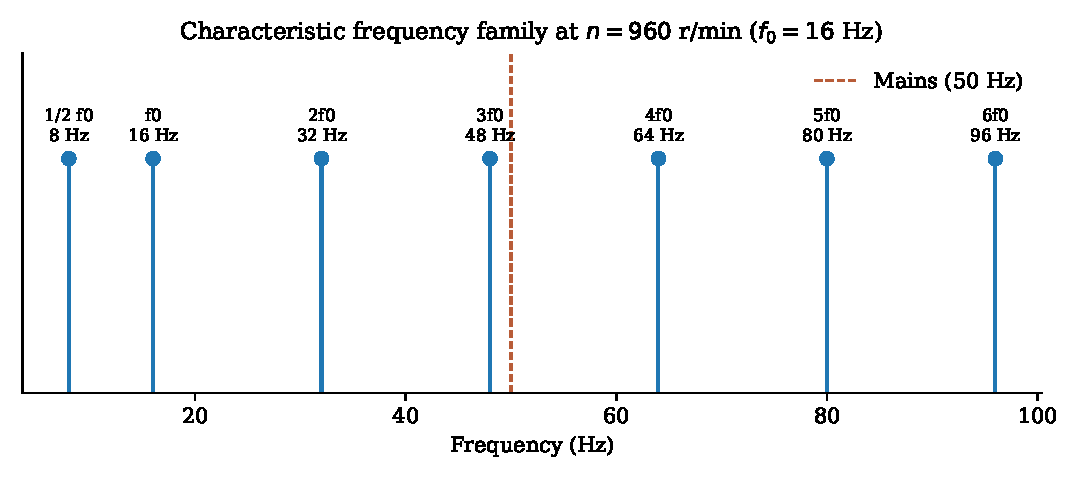
\includegraphics[width=0.92\textwidth]{harmonics.pdf}
\caption{Characteristic frequency family of the vertical axial-flow pump at \(960\,\mathrm{r/min}\). The dashed line is the supply frequency reported as interference in the healthy spectrum.}
\label{fig:harmonics}
\end{figure}

\begin{figure}[H]
\centering
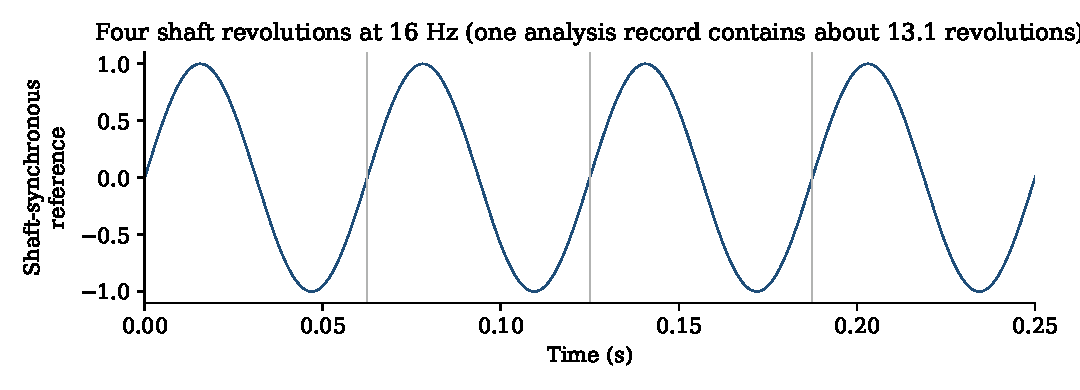
\includegraphics[width=0.92\textwidth]{shaft_cycles.pdf}
\caption{Shaft-synchronous reference at \(16\,\mathrm{Hz}\). A record of \(8192\) samples at \(10\,\mathrm{kHz}\) lasts \(0.8192\,\mathrm{s}\) and contains about \(13.1\) revolutions.}
\label{fig:cycles}
\end{figure}

\subsection{Frequency-domain analysis and the stationary assumption}

The discrete Fourier transform of a length-\(N\) record is
\begin{equation}
X[k]=\sum_{n=0}^{N-1} x[n]\,e^{-j 2\pi k n/N},\qquad
k=0,\ldots,N-1,
\label{eq:dft}
\end{equation}
and the one-sided periodogram used as a power estimate is
\begin{equation}
\hat{P}[k]=\frac{1}{N}\abs{X[k]}^{2}.
\label{eq:periodogram}
\end{equation}
Cooley and Tukey's algorithm~\cite{cooley1965} evaluates \eqref{eq:dft} in \(O(N\log N)\) operations, which is why a spectrum has been the default picture of a machine since the nineteen-sixties.
Parseval's relation says that the energy is conserved,
\begin{equation}
\sum_{n=0}^{N-1}\abs{x[n]}^{2}=\frac{1}{N}\sum_{k=0}^{N-1}\abs{X[k]}^{2},
\label{eq:parseval}
\end{equation}
so a spectrum is a redistribution of the same energy, not a new measurement.
Its bin spacing is \(\Delta f=f_{s}/N\).
At \(f_{s}=10\,\mathrm{kHz}\) and \(N=8192\), \(\Delta f=1.2207\,\mathrm{Hz}\).
That spacing resolves \(48\,\mathrm{Hz}\) from \(50\,\mathrm{Hz}\) and places each member of \(\mathcal{F}\) in its own bin.
Welch's averaged, windowed periodogram~\cite{welch1967,oppenheim1999,bendat2010} reduces the variance of \eqref{eq:periodogram} by splitting the record into overlapping segments, at the cost of a coarser \(\Delta f\).
For a \(0.82\,\mathrm{s}\) pump record the loss of resolution is expensive, and a single full-length transform is the more informative of the two.

The Fourier transform is the right tool when the signal is a sum of steady sinusoids plus stationary noise.
It is the wrong final tool when the fault is an impact that exists for a millisecond, or a modulation that turns on and off inside the record.
The transform then smears the transient across every bin and reports only the average spectrum.
Early pedestal looseness and early seal wear are of this second kind: the source study says explicitly that the weak fault is easily submerged in the periodic carrier and in the interference, and that a Fourier method alone is not accurate on the nonstationary vibration of a high-speed rotor.
The mathematical statement of the limitation is the uncertainty relation.
A window of duration \(T_{w}\) cannot localize time more tightly than \(T_{w}\) nor frequency more tightly than about \(1/T_{w}\).
The short-time Fourier transform
\begin{equation}
X(t,\omega)=\int_{-\infty}^{\infty} x(\tau)\,w(\tau-t)\,e^{-j\omega\tau}\,\mathrm{d}\tau
\label{eq:stft}
\end{equation}
makes the compromise explicit by fixing the window \(w\).
A narrow \(w\) sees the impact and loses the harmonic; a wide \(w\) sees the harmonic and loses the impact.
Wavelets refuse the fixed compromise.

\subsection{Wavelets, energy across scales, and empirical modes}

A wavelet is a zero-mean, finite-energy waveform \(\psi\), normalized so that \(\norm{\psi}_{2}=1\), and localized in time.
The continuous transform
\begin{equation}
W_{x}(a,b)=\frac{1}{\sqrt{\abs{a}}}\int_{-\infty}^{\infty} x(t)\,\psi^{*}\!\left(\frac{t-b}{a}\right)\mathrm{d}t
\label{eq:cwt}
\end{equation}
compares the signal with copies of \(\psi\) stretched by the scale \(a\) and shifted by the time \(b\).
Large \(a\) matches slow components; small \(a\) matches sharp ones.
Grossmann and Morlet~\cite{grossmann1984} introduced the transform for exactly the signals that a fixed window mishandles.
Dyadic sampling \(a=2^{j}\), \(j\in\mathbb{Z}\), keeps the construction invertible and, with a suitable \(\psi\), orthonormal.
Mallat's multiresolution analysis~\cite{mallat1989,daubechies1988,newland1993} implements that sampling as a pair of quadrature mirror filters.
If \(h\) is the low-pass filter associated with the scaling function \(\varphi\) and \(g\) is the high-pass filter associated with \(\psi\), one step of analysis is
\begin{align}
cA^{j}[k]&=\sum_{n} cA^{j-1}[n]\,h^{*}[n-2k],&
cD^{j}[k]&=\sum_{n} cA^{j-1}[n]\,g^{*}[n-2k].
\label{eq:mallat}
\end{align}
The detail coefficients \(cD^{j}\) are the dyadic wavelet transform at scale \(2^{j}\).
Reconstruction inserts the even-indexed coefficients back through the synthesis filters and adds the two branches.
Because each step retains half the samples, a length-\(N\) record yields about \(N\) coefficients in all, and the cost is linear in \(N\).
Chapter~\ref{ch:methods} writes the energy of each detail and the power spectrum of the strongest detail; those two formulae are the wavelet half of VWC.
What matters at the level of principle is that the scale axis is logarithmic.
One filter bank covers the impact band and the shaft band without having to choose a single STFT window.

Empirical mode decomposition, introduced by Huang and co-authors~\cite{huang1998}, takes a different route to the same nonstationary record.
It extracts intrinsic mode functions by repeated sifting: subtract the mean of the upper and lower envelopes until the result has a symmetric envelope and a number of extrema that differs from the number of zero crossings by at most one.
The signal becomes
\begin{equation}
x(t)=\sum_{i=1}^{M} c_{i}(t)+r(t),
\label{eq:emd}
\end{equation}
and a Hilbert transform of each \(c_{i}\) supplies an instantaneous frequency.
The decomposition is adaptive and does not need a mother wavelet.
It is also empirical: mode mixing, end effects, and a dependence on the sampling grid are well documented, and the review of Lei, Lin, He, and Zuo~\cite{lei2013} is largely a catalogue of those difficulties together with the repairs (ensemble EMD, noise-assisted variants) that followed.
Local mean decomposition and variational mode decomposition are later members of the same family.
The pump method does not use them.
It stays with the dyadic wavelet because the scale partition is fixed, the energy identity is exact up to the filter-bank orthogonality, and the maximum-energy scale is a well-defined index rather than a mode that may swap places between two records of the same fault.

\subsection{From a feature vector to a decision}

Once a record has been reduced to a vector \(\vect{x}\in\R^{d}\), diagnosis is a classification problem.
In the pump study \(d=22\) and the label \(y\) belongs to a set of four states.
A decision rule is a function \(f\) from \(\R^{d}\) to that set, learned from a finite training collection
\begin{equation}
\mathcal{T}=\bigl\{(\vect{x}_{i}, y_{i})\bigr\}_{i=1}^{n}.
\label{eq:trainingset}
\end{equation}
Two facts about \(\mathcal{T}\) dominate the choice of \(f\).
First, \(n\) is small.
The pump experiment yields \(60\) vectors per state and spends \(45\) of them on training, so \(n=180\) in \(22\) dimensions.
A richly parameterized neural network can interpolate \(\mathcal{T}\) and still fail on the \(60\) held-out vectors.
Second, the classes overlap.
Bearing-pedestal records are contaminated by resonance and by site interference, and every method in the published comparison loses more of those vectors than of the healthy ones.

Vapnik's statistical learning theory~\cite{vapnik1995,cortes1995,cover1965} answers the small-sample fact with a capacity control.
The probability of a large gap between training error and test error is bounded by a term that grows with the VC-dimension of the hypothesis class and shrinks with \(n\).
A hyperplane in a feature space of huge dimension would have a huge VC-dimension if it were unconstrained.
The support vector machine constrains it by maximizing the margin, and the kernel trick realizes that hyperplane in a space the user never writes down.
The practical price is two continuous parameters: the soft-margin penalty, which decides how many training points may fall inside the margin, and the width of the radial basis, which decides how finely the kernel measures distance.
Set either of them badly and the capacity-control argument no longer describes the machine that was actually trained.
Parameter search is therefore part of the classifier, not a preliminary inconvenience.
Grid search, genetic algorithms, particle swarm optimization, artificial bee colony search, chemical-reaction search, and shuffled frog-leaping search are all attempts to set those two numbers from the training data alone.
Section~\ref{sec:prior} compares them by the way they move through the parameter space.
Section~\ref{sec:problem} states why the unmodified frog-leaping search is not yet a satisfactory mover, which is the reason for the modification developed in Chapter~\ref{ch:methods}.

\subsection{What the technology chain must guarantee}

The principles above impose five obligations on any system that claims to diagnose this pump.

\begin{enumerate}
\item The sensor and the clock must be fast enough for the band they claim to see, and slow enough that the record still contains many shaft revolutions.
At \(10\,\mathrm{kHz}\) and \(8192\) samples the record holds about \(13.1\) revolutions and resolves the mains line from \(3f_{0}\).
That pair of facts is the acquisition specification.
\item The feature map must retain intensity, because severity is the standardized measure of damage, and it must retain the distribution of energy across \(\mathcal{F}\) in three directions, because severity does not separate the classes.
\item The feature map must be able to notice a weak transient that a single full-length Fourier transform would average away.
A dyadic energy spectrum is one construction that does so without giving up an exact notion of scale.
\item The classifier must be stable at \(n=180\), \(d=22\), four classes.
Margin methods meet that requirement more naturally than unrestricted multilayer networks.
\item The parameters of the classifier must be chosen by a search that does not collapse onto the first strong training vector it finds.
On a \(60\)-vector test set, a five-point swing in accuracy is three samples.
A search that overfits the training fold will spend those three samples.
\end{enumerate}

The rest of the chapter asks how far the published literature has already carried these five obligations, and where it stops short of the pump problem as posed by You and co-authors.

\section{Previous work on features, classifiers, and their combination}
\label{sec:prior}

The literature is large enough that a flat list of papers would hide the structure.
The review is organized by the technical idea each line contributed, and each idea is tied back to one of the five obligations above.
Citations concentrate on rotating machinery, with the neighboring lines (inverters, process plants, heat pumps) included only where the same classifier or the same fusion argument was developed and later imported.

\subsection{Symptom catalogues and analytic redundancy}

The oldest diagnostic tradition is a catalogue of symptoms written by people who had dismantled failed machines.
Sohre's account of high-speed turbomachinery~\cite{sohre1968,rao2011} sorts operating problems into a small number of mechanical families---unbalance, misalignment, looseness, rub, bearing damage, resonance, and a handful of hydraulic and aerodynamic mechanisms---and lists the spectral clues an analyst should expect from each.
The nine-family, thirty-seven-type partition cited in the source paper is this kind of catalogue.
It remains the right vocabulary for the four pump states.
Eccentric axle is unbalance.
Bearing pedestal is a looseness that begins in a rolling-element fault.
Sealing-ring wear is a hydraulic leakage that loads the rotor.
The catalogue tells the analyst which lines in \(\mathcal{F}\) ought to move.
It does not compute the lines, and it does not assign a new record automatically.

A second early tradition replaces the catalogue by a model.
Beard's thesis~\cite{beard1971} showed that a linear system can be fitted with analytic redundancy: a bank of observers, each of which assumes a different fault, produces a residual that is small only under its own assumption.
Willsky's survey and Frank's survey~\cite{willsky1976,frank1990} established residual generation as a discipline, with detection as a decision on the residual and isolation as a decision on which residual moved.
Sliding-mode observers, as developed by Edwards, Spurgeon, and Patton~\cite{edwards2000}, keep the residual well behaved when the plant is uncertain, by forcing the estimation error onto a surface in finite time.
Persis and Isidori~\cite{persis2001} gave geometric conditions under which a nonlinear system admits a filter that is sensitive to one fault and invariant to the others.
Isermann's review~\cite{isermann2005} then placed model-based detection next to the industrial systems that can actually support it: the model has to be accurate in the frequency band of the fault, the disturbances have to be characterizable, and the sensors have to observe the states the residual needs.

For a vertical axial-flow pump in a closed water loop, that last requirement is the obstacle.
The forces in \eqref{eq:rotor} depend on the seal gap, the bearing clearance, the dissolved gas, and the precise pedestal stiffness, none of which is known to the accuracy a residual would need in order to be smaller than the fault.
The experiment measures casing acceleration and almost nothing else.
A data-driven front end is not a rejection of the model-based line.
It is what remains when the residual cannot be built.
The later numerical comparison is therefore entirely among data-driven classifiers that share one feature vector.

\subsection{Wavelet features for gears, bearings, and drives}

Peng and Chu's review of the wavelet transform~\cite{peng2004,jardine2006} in machine condition monitoring is the point at which wavelets stop being a mathematical import and become a standard feature tool.
The argument of that review is the one already used in Section~\ref{sec:principles}: a fault transient is localized in time, a Fourier coefficient is not, and the variable window of \eqref{eq:cwt} matches the transient at the scale where its energy actually sits.
Three constructions recur.

The discrete wavelet transform, implemented by \eqref{eq:mallat}, yields one energy per scale,
\begin{equation}
E_{j}=\sum_{k}\abs{cD^{j}[k]}^{2},
\label{eq:scaleenergy}
\end{equation}
and the vector \((E_{j})\) is the feature.
Saravanan and Ramachandran~\cite{saravanan2010} extract exactly this kind of description from an incipient gearbox vibration by the discrete wavelet transform, then hand the vector to an artificial neural network.
The network is there because the energy vector is not linearly separable by eye once the gearbox carries more than one fault type.
Hu, He, Zhang, and Zi~\cite{hu2007} improve the wavelet-packet variant, in which both the detail and the approximation are split at every level so that the frequency tiles are equal rather than dyadic, and they classify with an ensemble of support vector machines.
The packet transform is more flexible and more redundant; the dyadic transform used for the pump is the cheaper sibling, and it is enough when the question is only which scale dominates.

A second construction keeps the coefficients themselves, or a statistic of them, inside the band where a bearing resonance lives.
Lou and Loparo~\cite{lou2004} combine a wavelet step with a fuzzy inference on bearing records.
Gao and Yan~\cite{gao2011} systematize the same idea for manufacturing signals: choose the mother wavelet by its resemblance to the impulse, keep the scale whose kurtosis or energy is extreme, and only then compute a spectrum.
Spectral kurtosis, in Antoni's formulation~\cite{antoni2006}, is a related detector that does not need a wavelet at all.
It measures, in each frequency bin, the normalized fourth moment of the short-time Fourier amplitudes, and it peaks where the signal is impulsive.
The coefficient power spectrum of the maximum-energy wavelet level is a cousin of this idea.
First find the scale that holds the energy, then read the periodic structure inside that scale.
The pump method adds the severity scalar and the three-axis repetition, which spectral kurtosis by itself does not supply.

A third construction uses complex or continuous wavelets when the phase, not only the energy, carries the fault.
Seshadrinath, Singh, and Panigrahi~\cite{seshadrinath2014} apply complex wavelets to variable-frequency drives and show that several electrical and mechanical faults can be separated from the vibration signature when the transform preserves phase relations that a real orthogonal wavelet discards.
Khalil and Bayoumi~\cite{khalil2001} had earlier used a dyadic wavelet affine invariant for a different recognition task; the citation matters here because it records that the dyadic grid is stable under the shifts a real acquisition produces.
The pump records are triaxial acceleration at a fixed speed, not a variable-frequency electrical drive, so the simpler real dyadic energy is the appropriate member of the family.
The complex-wavelet result remains the warning that a phase-blind energy can fail when the fault is a change of timing rather than a change of intensity.

Bin, Gao, Li, and Dhillon~\cite{bin2012} combine wavelet packets with empirical mode decomposition for early rotor faults, then classify ten rotor states with a neural network.
The combination is a useful reference point because it admits, by existing, that neither the packet energies nor the modes are always sufficient alone.
VWC is a different combination: a time-domain standard (severity), a scale distribution (the energy time-spectrum), and a harmonic reading of the loudest scale (the coefficient power spectrum).
It is deliberately small.
Twenty-two numbers are the entire interface between the signal and the classifier.

\subsection{The empirical-mode line}

Lei, Lin, He, and Zuo~\cite{lei2013} review empirical mode decomposition in rotating-machine diagnosis and list the faults for which a mode energy, a mode entropy, or a Hilbert envelope spectrum has been used as a feature.
Dybała and Zimroz~\cite{dybala2014} show that the early stage of a rolling-bearing fault, still buried in the raw spectrum, becomes visible once the high-frequency mode that the impacts excite is isolated and demodulated.
Wu and Huang's ensemble empirical mode decomposition~\cite{wu2009} attacks the mode-mixing that made two records of the same fault produce differently ordered modes: each sift is run on the signal plus a different noise, and the modes are averaged.
Zhang, Liang, Zhou, and Zang~\cite{zhang2015} put permutation entropy of the ensemble modes beside an optimized SVM for bearings.
Zhao, Wang, Ma, and Li~\cite{zhao2016} use complete ensemble decomposition, a short-time Fourier entropy, and a multiclass SVM on a hydraulic pump, which is the closest industrial cousin of the axial-flow pump in this paper.
Yang, Liu, Li, Li, and Ma~\cite{yang2015,karaboga2007} extract gear features by the ensemble decomposition and classify them by an SVM whose parameters are set by an artificial bee colony.
Huang, Hu, and Yang~\cite{huang2011} do the same service for a high-voltage circuit breaker with the plain decomposition, an energy entropy, and a genetic algorithm around the SVM.

Two lessons travel from that line into the present design, and one does not.
The first lesson is that a demodulated or scale-local spectrum sees an early fault that the raw Fourier transform misses.
The coefficient power spectrum is the wavelet version of that lesson.
The second lesson is that the SVM, not the particular adaptive decomposition, is what turns the feature into a label when the sample is small, and that the SVM's two parameters are worth a global search.
The lesson that does not travel is the adaptive partition itself.
On sixty records per class, an adaptive mode ordering is an extra source of variance between the training fold and the test fold.
A fixed dyadic filter bank removes that variance.
The price is a bank that is not matched to each record.
The maximum-energy rule gives back a limited adaptivity: the scale index \(k\) may differ from record to record even though the filters do not.

Local mean decomposition, which Smith defined~\cite{smith2005} for nonstationary physiological signals and which Tian, Ma, Lu, and Wang later paired~\cite{tian2015} with a singular-value step and an extreme learning machine for bearings under variable conditions, belongs to the same adaptive family.
Variational mode decomposition, which Dragomiretskiy and Zosso posed~\cite{dragomiretskiy2014} as an optimization rather than a sift, has largely replaced ad-hoc sifting in newer work because the modes are concurrent and the bandwidth of each mode is a penalty term.
Neither is used here.
They are recorded so that the choice of a dyadic bank is visible as a choice.

\subsection{Neural networks trained on time-domain and spectral features}

Samanta and Al-Balushi~\cite{samanta2003} take time-domain statistics of bearing vibration in the healthy and the faulty states and present them to a multilayer perceptron.
The network learns a partition of that statistic space.
Samanta's later gear study~\cite{samanta2004} puts the same style of network beside an SVM and lets a genetic algorithm pick features and parameters for both, which is an early acknowledgement that the classifier and the feature set should be tuned together.
Li, Chow, Tipsuwan, and Hung~\cite{li2000} apply a neural network to motor rolling-bearing vibration and show that a time-frequency front end plus a network can track bearing condition on a test motor.
Huang and Xie~\cite{huang2009} use a backpropagation network on rolling bearings; their network is one of the three baselines in the pump comparison, so its inductive bias matters in detail.

A backpropagation network with one hidden layer models the label as a smooth nonlinear function of \(\vect{x}\).
With weights collected in \(\vect{\theta}\), training minimizes a squared or cross-entropy loss
\begin{equation}
J(\vect{\theta})=\frac{1}{n}\sum_{i=1}^{n} \ell\bigl(y_{i}, f_{\vect{\theta}}(\vect{x}_{i})\bigr)+\lambda\norm{\vect{\theta}}^{2}
\label{eq:bpnn}
\end{equation}
by gradient steps.
The model can represent the four pump states.
On \(180\) training vectors it can also represent accidents of the training split.
The published numbers, read in Chapter~\ref{ch:estimation}, show a training accuracy of \(91.7\%\) and a test accuracy of \(85.0\%\) for this baseline, a larger train-to-test drop than any of the SVM variants.
That drop is the capacity argument becoming visible in a table.
Kankar, Sharma, and Harsha~\cite{kankar2011} compare several machine-learning methods on ball bearings and reach the same practical conclusion from another data set: the method that controls its capacity generalizes better when the faulty examples are few.
Jack and Nandi's comparison of SVMs and neural networks~\cite{jack2002}, both augmented by a genetic algorithm, is the gearbox version of the same conclusion.

Deep and multimodal extensions exist.
Li, Sanchez, Zurita, Cerrada, Cabrera, and Vásquez~\cite{li2015deep} build a multimodal deep support vector classifier for spur and helical gearboxes, using homologous features from several sensors.
The pump study has three axes, which is a weak form of the same idea, but it fuses them by concatenation into the \(22\)-vector rather than by a deep stack.
With sixty examples per class a deep stack is not identified.
The baseline that the source actually trains is the shallow backpropagation network, and that is the neural result this paper interprets.

\subsection{Support vector machines and the search for their parameters}

Cortes and Vapnik's soft-margin classifier~\cite{cortes1995}, and the earlier hard-margin algorithm of Boser, Guyon, and Vapnik~\cite{boser1992}, are the decision rule used for the pump once the features exist.
Widodo and Yang's review~\cite{widodo2007,lei2008} collects the first decade of that rule in condition monitoring: bearing faults, gear faults, induction machines, and pumps, with linear, polynomial, and radial kernels, and with the repeated observation that the radial kernel is the one practitioners keep.
The geometry and the dual problem are derived in Section~\ref{sec:svm}.
The prior art that matters here is the outer loop that chooses the penalty \(C\) and the kernel width.

A grid search evaluates \(C\) and the width on a logarithmic lattice and keeps the pair with the best cross-validated accuracy.
It is simple, and it is expensive in the number of trainings.
It also cannot spend evaluations where the surface is interesting, because the lattice is chosen in advance.
Bordoloi and Tiwari~\cite{bordoloi2014,holland1975} compare a grid, a genetic algorithm, and an artificial bee colony on a four-class gear problem, which is the same number of classes as the pump, and find that the evolutionary searches reach accurate multi-fault partitions.
Holland's genetic algorithm maintains a population of candidate pairs, selects the accurate ones, and recombines them.
Its operators do not use the slope of the accuracy surface, which is an advantage because cross-validated accuracy is a step function of \(C\) and of the width.
Kennedy and Eberhart's particle swarm~\cite{kennedy1995} moves each candidate toward its own best position and toward the swarm's best position, with a momentum term.
Dong and Luo~\cite{dong2013,suykens1999} use that swarm to set the parameters of a least-squares SVM, after a principal-component compression, for bearing degradation prediction.
Suykens and Vandewalle's least-squares variant replaces the inequality constraints of the standard SVM by equalities, so the training step is a linear system.
It is faster and it loses the sparse set of support vectors.
The pump classifier stays with the standard soft-margin dual.

Karaboga's artificial bee colony searches by employed bees, onlookers, and scouts, and it is the optimizer inside Yang's gear classifier.
Alatas's artificial chemical reaction optimization~\cite{alatas2011} treats candidate solutions as molecules and moves them by synthesis, decomposition, and collision reactions.
Ao, Cheng, Li, and Truong~\cite{ao2014} wrap that reaction search around an SVM for roller bearings, with a local characteristic-scale energy entropy as the feature.
Their ACROA-SVM is the second baseline of the pump study.
It is a strong baseline: on the published test set it ties the unmodified frog-leaping SVM at \(91.7\%\) pooled accuracy.

The shuffled frog-leaping algorithm of Eusuff and Lansey, later elaborated with Pasha~\cite{eusuff2003,eusuff2006}, was built for discrete water-network design and then used as a general memetic search.
A population of frogs is partitioned into memeplexes.
Inside a memeplex the worst frog leaps toward the best frog of that memeplex, and if the leap fails, toward the best frog of the whole population.
If that also fails, the worst frog is replaced at random.
Memes, in the sense of the memetic algorithm, are the local improvements; the shuffle that follows the local search is the global mixing, inherited in spirit from the particle swarm.
The appeal, as the source paper states it, is a short parameter list, a simple leap, and a search that is partly local and partly global.
The defect, also stated there, appears as the iteration count grows.
Frogs converge, the memeplexes stop differing from one another, and the random replacement of a failed frog is a blind jump that throws away the position already reached.
The modified leap in Chapter~\ref{ch:methods} is aimed at those two defects and at nothing else.
It does not change the SVM.
It changes the way \(C\) and the kernel parameter are proposed.

A practical guide belongs in this review because the search is only as good as the training procedure inside it.
Chang and Lin's LIBSVM~\cite{chang2011,platt1999} is the standard solver for the dual, using Platt's sequential minimal optimization on pairs of multipliers.
Hsu, Chang, and Lin's guide~\cite{hsu2003} fixes the conventions that the search must respect: scale each feature to a common range before training, search \(C\) and the radial width on a log grid first so that the evolutionary search has a sane box, and judge candidates by cross-validation rather than by training accuracy.
The pump pipeline normalizes before classification, which is the first of those conventions.
The fitness of a frog is a cross-validated classification rate, which is the third.
The source study does not publish the box over which \(C\) and the width were searched.
The exposition in Chapter~\ref{ch:methods} therefore states the box as an algorithmic object and does not pretend to recover a number the experiment never printed.

Schölkopf and Smola's kernel monograph~\cite{scholkopf2002,mercer1909} supplies the positive-definiteness condition, going back to Mercer, that lets the radial basis be a kernel at all.
Without that condition the dual quadratic program need not be convex and the solver's output need not be a margin maximizer.
The radial basis used here satisfies the condition for every positive width, so the only remaining question is which width, together with which penalty, the leap should return.

\subsection{Fusion, Bayesian networks, and neighboring plants}

Not every fault is carried by one vibration sensor.
Cai, Huang, and Xie~\cite{cai2017bn} review Bayesian networks as a way to fuse uncertain symptoms: each node is a fault or a test, and the edges are conditional probabilities that a test is positive given a fault.
Cai, Liu, Fan, and co-authors~\cite{cai2014} apply that construction to a ground-source heat pump, fusing several information sources, and report a clear gain over a single-source decision.
Cai, Zhao, Liu, and Xie~\cite{cai2017inv} later give a data-driven Bayesian treatment of inverter faults in a permanent-magnet drive.
Yin, Zhu, and Kaynak~\cite{yin2015} keep a partial least-squares model and focus the detection statistic on the key performance indicators of the plant rather than on every measured channel equally.
Venkatasubramanian's three-part review~\cite{venkat2003} of process fault detection places these ideas in a larger map: quantitative model residuals, qualitative symptom reasoning, and historical data methods.

The axial-flow pump experiment is a historical-data method with a single triaxial sensor.
It does not estimate a Bayesian network.
The fusion it does perform is early fusion, inside the feature vector: three directions, seven harmonics, one severity.
The heat-pump result is relevant as a ceiling.
When independent symptoms exist, a network that multiplies their likelihoods can beat a classifier that sees only vibration.
The published pump comparison does not have those extra symptoms, so the ceiling is not available, and the gains reported in Chapter~\ref{ch:estimation} are gains of feature and of parameter search only.

A number of SVM papers in the source bibliography sit outside rotating machinery: open-circuit detection in drives, intrusion detection, vehicle suspension, biochemical processes.
They establish that the same \((C, \text{width})\) problem appears whenever an SVM is the decision rule.
They are not evidence about pumps.
This review uses them only to support the narrow claim that parameter search is part of the method.

\subsection{What the previous work has already settled}

The lines above agree on more than they dispute.

\begin{itemize}
\item Spectral symptoms organized by shaft order are the right language for unbalance, looseness, and hydraulic once-per-revolution faults.
Sohre's catalogue and the bearing kinematics \eqref{eq:bearing} are still the interpretation layer sitting on top of any classifier.
\item A fixed-window spectrum is a weak detector of early impulsive faults.
Wavelet energies, wavelet-packet energies, spectral kurtosis, and empirical-mode envelope spectra are the repairs, and they work for the same reason.
\item On a few hundred labeled records, a margin classifier with a radial kernel is a stronger default than an unrestricted neural network.
The published pump tables reproduce this general experience.
\item The radial SVM does not choose its own penalty and width.
Grid search, genetic algorithms, particle swarms, bee colonies, chemical-reaction search, and frog-leaping search are all credible outer loops, and on gear and bearing benchmarks the evolutionary loops beat a coarse grid.
\item Fusion of independent sensors helps when the sensors exist.
A triaxial accelerometer is a minimal fusion, and it is the one the pump rig provides.
\end{itemize}

\section{The problem this paper addresses}
\label{sec:problem}

\subsection{The gap between the settled results and the pump}

The settled results do not by themselves diagnose the vertical axial-flow pump.
Four concrete gaps remain, and they are the problem statement.

The first gap is the feature gap.
Severity is standardized and, on this rig, almost blind to the pedestal fault: \(1.161\,\mathrm{mm/s}\) against \(1.051\,\mathrm{mm/s}\) in the healthy state.
A Fourier spectrum sees the healthy blade-pass line at \(64\,\mathrm{Hz}\) and the supply line at \(50\,\mathrm{Hz}\), and it averages any transient that does not last for the whole \(0.82\,\mathrm{s}\) record.
A wavelet energy vector sees which scale is loud and does not say whether the loudness is at \(8\,\mathrm{Hz}\) or at \(16\,\mathrm{Hz}\).
An empirical mode may say both and may order itself differently on the next record.
The missing object is a short vector that contains the standardized intensity, the scale distribution, and the shaft-order reading of the loudest scale, taken in the three directions the casing sensor actually measures.
VWC is that object.
It is defined so that the four states reported in the source---healthy concentration at \(f_{0}\), eccentric growth of that line and of the severity, pedestal growth of \(\tfrac12 f_{0}\), seal-wear growth of \(\tfrac12 f_{0}\) and \(2f_{0}\)—are different points in the same \(\R^{22}\).

The second gap is the stationarity gap, stated in the source introduction and repeated here as an obligation.
The vibration of the pump under an early fault is a strong periodic carrier plus a weak, nonstationary disturbance plus interference.
Methods whose only transform is \eqref{eq:dft} are, on the source authors' own account, inaccurate for that mixture.
The method has to analyze the record in time and in scale, and it still has to return the harmonic amplitudes a mechanical interpretation requires.
The energy time-spectrum followed by a coefficient power spectrum is a specific answer to that double requirement.
Chapter~\ref{ch:methods} writes the answer in equations and fixes the implementation choices the source text leaves implicit.

The third gap is the search gap.
The shuffled frog-leaping algorithm already combines a local leap and a global leap, which is why it is a reasonable optimizer for \((C, g)\).
As the source formulates the defect: once frogs begin to agree, diversity collapses, the search sits in a local optimum of the cross-validated accuracy, and a failed frog is replaced by a uniform random draw that does not use the position it is abandoning.
On a fitness surface that is a step function of two parameters, a blind draw is not a rare event, and each draw costs a full cross-validated training.
The modification has to do two things and stop.
It has to let the worst frog learn from the local leader and the global leader in the same leap, with weights that depend on how far the frog is from the global leader, so that a frog already near the leader exploits and a frog far from the leader explores.
It has to replace the blind draw by a Gaussian perturbation of the current position, so that a failed leap becomes a local mutation rather than a restart.
Both changes are internal to the leap.
The fitness function remains the cross-validated SVM accuracy, and the decision function remains the radial-basis SVM.
MSFLA is that modified leap.

The fourth gap is the evaluation gap.
A method that is only a derivation is not yet a diagnosis.
The pump rig supplies four states that a reader can understand mechanically, a sample that is honestly small, and three published baselines: the backpropagation network, the chemical-reaction SVM, and the unmodified frog-leaping SVM.
The problem includes reading that comparison at the resolution the tables support.
Overall accuracy hides the pedestal state, which is the worst class for every method.
Training accuracy hides the generalization drop, which is largest for the neural baseline.
A single pooled percentage hides the fact that the entire test set is sixty vectors, so a difference of one vector is \(1.7\) percentage points.
Chapter~\ref{ch:estimation} performs that reading.
It does not invent a second experiment.

\subsection{Objectives}

The paper has four objectives, matched to the four gaps.

\begin{enumerate}
\item Derive and specify the VWC map from a triaxial acceleration record to a vector in \(\R^{22}\): the severity, the dyadic energy time-spectrum, the selection of the maximum-energy level, and the coefficient power spectrum at the seven shaft orders on three axes.
\item Derive the soft-margin SVM with a radial kernel, then specify the modified frog-leaping search that sets its penalty and its kernel parameter, including the distance-weighted leap and the Gaussian mutation, and state which quantities the published experiment does not report.
\item Describe the acquisition system as a build: the closed water loop, the four mechanical states, the triaxial charge sensor, the sampling clock, the record length, and the split into \(180\) training vectors and \(60\) test vectors.
\item Estimate performance from the published counts.
Report per-class and pooled rates, the train-to-test drop of each method, and the special difficulty of the bearing-pedestal state, with the arithmetic of the tables made explicit.
\end{enumerate}

\subsection{What is deliberately outside the problem}

A precise problem also says what it will not claim.
This paper does not claim a new laboratory campaign.
The severities, the hardware table, and the classification counts come from You, Fan, Li, Liang, Fang, and Wang.
Illustrative signals in the figures are synthetic records scaled to those severities and shaped to the harmonic patterns the source describes; each such figure is captioned as illustrative.
The paper does not claim that MSFLA is a universal optimizer, or that VWC is the unique admissible front end.
Packet energies, spectral kurtosis, and ensemble modes remain legitimate alternatives where the sample and the hardware differ.
The paper does not claim a detection delay, a remaining-useful-life estimate, or a performance under variable speed.
The rig runs at one stated speed, \(960\,\mathrm{r/min}\).
The paper does not claim an optimal \(C\) or an optimal kernel width, because the source does not print them.
It claims that the search procedure is fully specified and that the published accuracy table is the estimate of its worth on this rig.

\subsection{Map of the remaining chapters}

Chapter~\ref{ch:methods} answers the first two objectives.
Section~\ref{sec:vwc} builds the feature map from the velocity integral through the Mallat bank to the \(22\)-vector, and it interprets each block against the four mechanical states.
Section~\ref{sec:svm} builds the classifier from the hard-margin geometry through the radial dual to the modified leap, and it writes the algorithm as a procedure that can be implemented without consulting the source text for missing formulae.
Chapter~\ref{ch:estimation} answers the last two objectives.
Section~\ref{sec:build} specifies the rig, the sensor chain, the sampling arithmetic, and the software path from a record to a label.
Section~\ref{sec:estimate} reads the feature signatures and the classification tables, states the strength of the estimate, and lists the limits that a sixty-vector test set imposes.
The two technologies are separable.
A reader who already trusts the \(22\)-vector can substitute another outer-loop optimizer.
A reader who already has MSFLA can point it at another front end.
The paper evaluates them as the pair the source proposed, because that is the pair for which a published estimate exists.

\begin{figure}[H]
\centering
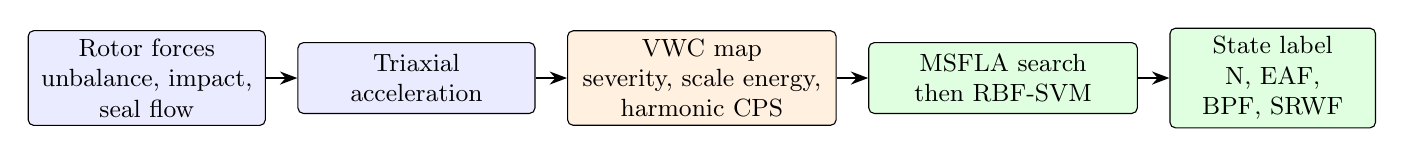
\begin{tikzpicture}[
  box/.style={draw, rounded corners=2pt, align=center, minimum height=9mm, inner sep=3pt, font=\small},
  arr/.style={-{Stealth[length=2.2mm]}, thick}
]
\node[box, fill=blue!8, text width=28mm] (force) {Rotor forces\\unbalance, impact,\\seal flow};
\node[box, fill=blue!8, text width=28mm, right=4mm of force] (sens) {Triaxial\\acceleration};
\node[box, fill=orange!12, text width=32mm, right=4mm of sens] (vwc) {VWC map\\severity, scale energy,\\harmonic CPS};
\node[box, fill=green!12, text width=32mm, right=4mm of vwc] (svm) {MSFLA search\\then RBF-SVM};
\node[box, fill=green!12, text width=24mm, right=4mm of svm] (lab) {State label\\N, EAF,\\BPF, SRWF};
\draw[arr] (force) -- (sens);
\draw[arr] (sens) -- (vwc);
\draw[arr] (vwc) -- (svm);
\draw[arr] (svm) -- (lab);
\end{tikzpicture}
\caption{The diagnostic chain addressed by this paper. Chapter~\ref{ch:previous} covers the forces and the sensor. Chapter~\ref{ch:methods} covers the two computational blocks. Chapter~\ref{ch:estimation} covers the rig that produces the acceleration and the estimate of the label.}
\label{fig:chain}
\end{figure}

\chapter{The Two Diagnostic Technologies}
\label{ch:methods}

The diagnosis is a composition of two maps.
The first map, VWC, sends a triaxial acceleration record to a point in \(\R^{22}\).
The second map, MSFLA-SVM, sends that point to one of four labels, after a search has fixed the two parameters of a radial-basis support vector machine.
This chapter specifies both maps at the level of equations, algorithms, and implementation choices.
Where the source study leaves a choice unspecified, the choice is stated and marked as a specification of this exposition rather than as a recovered experimental setting.

\section{Technology one: the VWC feature map}
\label{sec:vwc}

\subsection{What the map is required to preserve}

Let one observation be three finite sequences
\begin{equation}
a_{r}[n],\ a_{t}[n],\ a_{a}[n],\qquad n=0,\ldots,N-1,
\label{eq:triaxial}
\end{equation}
sampled at \(f_{s}\), together with the shaft speed \(n_{\mathrm{rpm}}\) that fixes \(f_{0}\) through \eqref{eq:f0}.
On the published rig, \(f_{s}=10\,\mathrm{kHz}\), \(N=8192\), and \(n_{\mathrm{rpm}}=960\).
The map
\begin{equation}
\Phi:\ (a_{r}, a_{t}, a_{a})\ \longmapsto\ \vect{x}\in\R^{22}
\label{eq:phi}
\end{equation}
has to preserve three different facts at once.
The first fact is how hard the machine is vibrating, in the standardized sense of root-mean-square velocity.
The second fact is how that vibration is spread across time scales, so that a short-lived transient is not averaged into invisibility.
The third fact is how the energy of the loudest scale is distributed among the seven shaft orders in \eqref{eq:family}, because those orders are the mechanical vocabulary of the four states.
VWC is the conjunction of those three facts: vibration severity, the dyadic wavelet energy time-spectrum, and the coefficient power spectrum of the maximum-energy level.
The initial letters of the three blocks name the map.

The blocks are complementary in a precise sense.
Severity is invariant to a redistribution of energy among frequencies, which is why the pedestal fault hides inside it.
The energy time-spectrum is invariant to a redistribution among frequencies that share a scale, which is why two different shaft orders inside one dyadic band produce the same \(E_{j}\).
The coefficient power spectrum breaks that remaining invariance, at the price of being computed on only one scale.
Using the maximum-energy scale concentrates the third block where the record actually has energy, instead of averaging a spectrum over scales that contain only the noise floor.

\subsection{Vibration severity}

The continuous definition \eqref{eq:vibcont} and the discrete RMS \eqref{eq:vibdisc} are the first block.
The velocity series that enters \eqref{eq:vibdisc} is obtained from acceleration.
This exposition distinguishes the source formula from the integrator used to scale the illustrative figures.

The source formula accumulates absolute acceleration over a window of \(10\,\mathrm{ms}\),
\begin{equation}
v_{i}=\int_{0}^{0.01}\abs{a_{i}(t)}\,\mathrm{d}t.
\label{eq:vsrc}
\end{equation}
On a uniform grid with step \(\Delta t=1/f_{s}\) the integral is a sum of \(0.01 f_{s}\) samples.
At \(10\,\mathrm{kHz}\) that is \(100\) samples.
The absolute value makes \(v_{i}\) nonnegative and proportional to the local mean absolute acceleration.
Substituting the resulting series into \eqref{eq:vibdisc} produces the severity that the source reports: \(1.051\,\mathrm{mm/s}\) healthy, \(3.737\,\mathrm{mm/s}\) for the eccentric axle, \(1.161\,\mathrm{mm/s}\) for the bearing pedestal, and \(1.70024\,\mathrm{mm/s}\) for sealing-ring wear, all quoted for the radial direction in which the time-domain figures of the source are drawn.
Figure~\ref{fig:severity} restates those four numbers.
The eccentric state is more than three times the healthy severity.
The pedestal state is about ten percent above healthy.
A threshold on severity alone can flag the eccentric axle and cannot reliably flag the pedestal.

\begin{figure}[H]
\centering
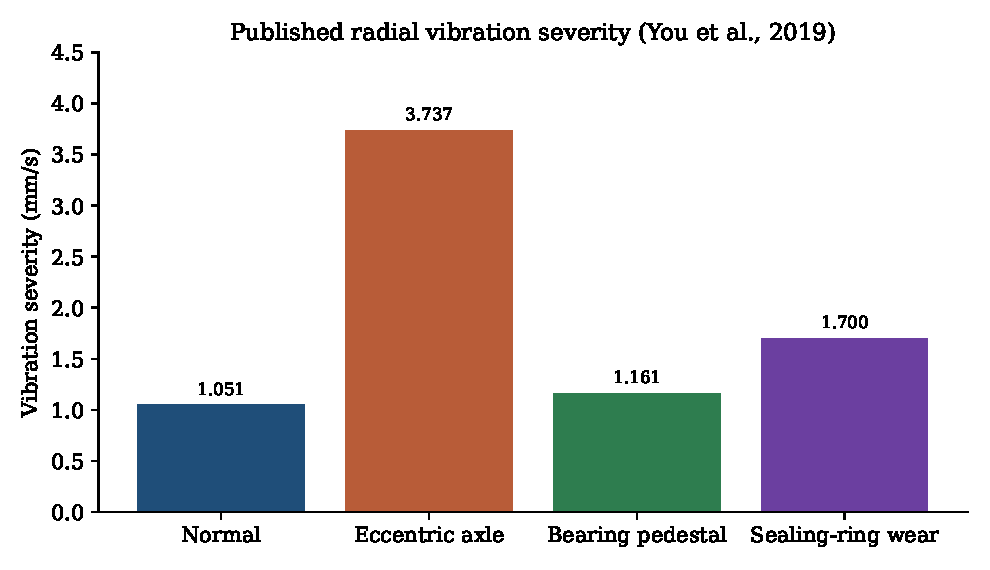
\includegraphics[width=0.78\textwidth]{severity.pdf}
\caption{Radial vibration severity reported by You et al.\ for the four operating states. These are published measurements, not quantities computed from the illustrative signals.}
\label{fig:severity}
\end{figure}

The illustrative waveforms of Figure~\ref{fig:waves} are built differently, and the difference is intentional.
Each synthetic acceleration is high-pass integrated,
\begin{equation}
\tilde{v}[n]=\Delta t\sum_{k=0}^{n} a[k],\qquad
v=\mathcal{H}_{2\,\mathrm{Hz}}\{\tilde{v}\},
\label{eq:illustvel}
\end{equation}
and the acceleration is scaled by a single positive constant until \(\sqrt{\tfrac{1}{N}\sum v[n]^{2}}\), expressed in millimetres per second, equals the published severity of that state.
The shape of each record---a shaft-locked fundamental, a half-order where the source describes one, a blade-pass component, a weak supply tone in the healthy state, and a resonance near \(200\,\mathrm{Hz}\) that gives the dyadic bank something to localize---follows the qualitative signatures of Section~\ref{sec:signatures}.
The samples are not a reconstruction of the laboratory series, whose raw values are not in the source paper.
They exist so that the later formulae can be looked at on a signal whose intensity and whose harmonic emphasis agree with the published description.

\begin{figure}[H]
\centering
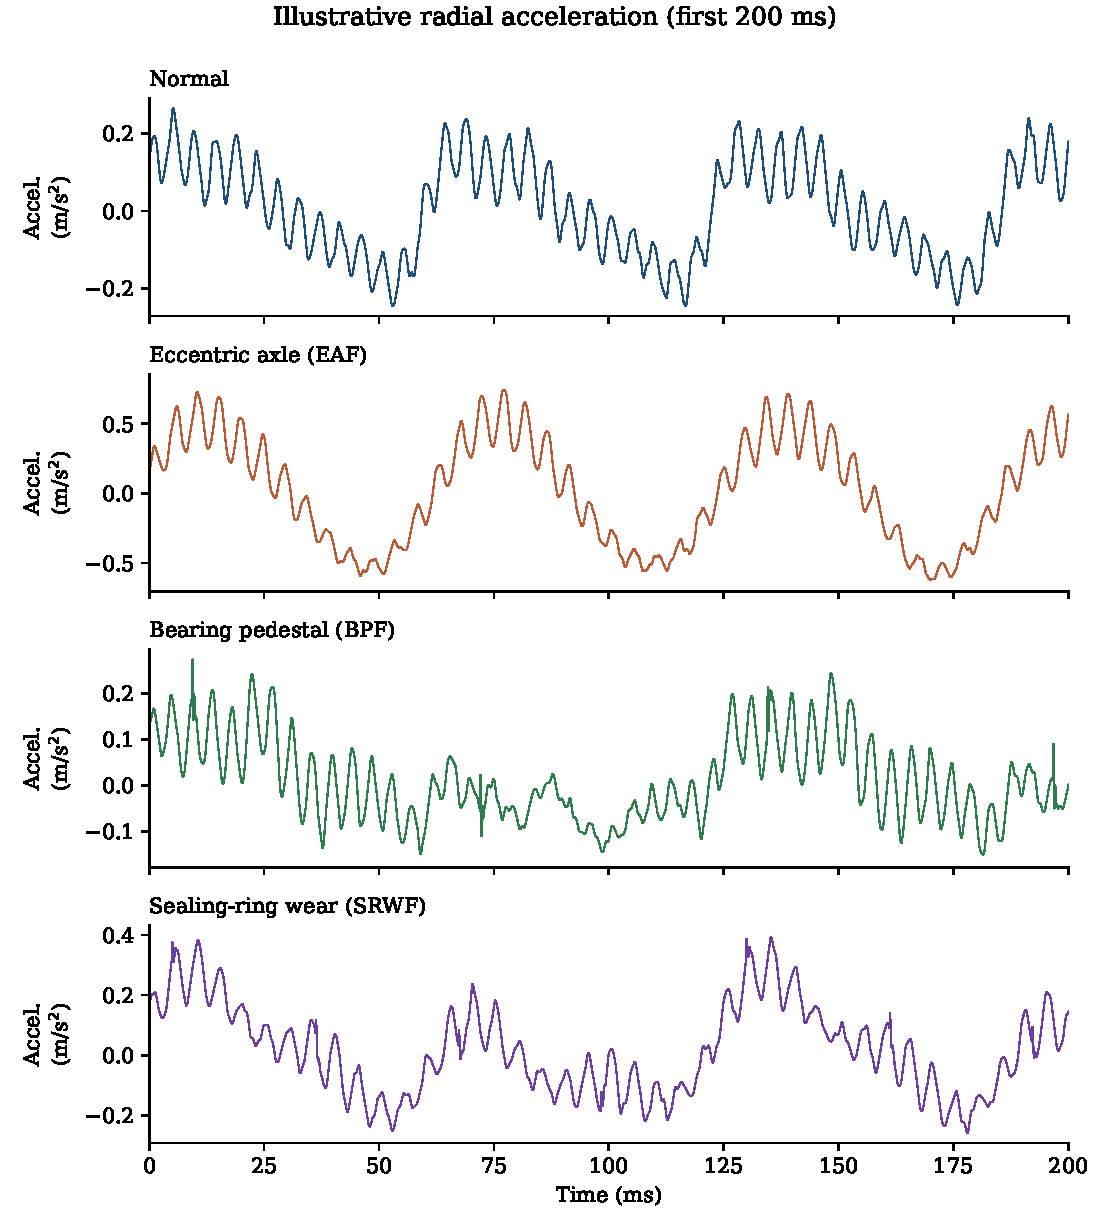
\includegraphics[width=0.92\textwidth]{waveforms.pdf}
\caption{Illustrative radial acceleration over the first \(200\,\mathrm{ms}\). Each record is scaled so that the RMS of its high-pass-integrated velocity equals the published severity of that state.}
\label{fig:waves}
\end{figure}

Severity contributes one coordinate to \(\vect{x}\), not three.
The arithmetic of the source is explicit: seven harmonics in three directions give \(21\) spectral coordinates, and the full vector has dimension \(22\), so exactly one severity is appended.
Figure~8 of the source shows that coordinate in the radial direction across groups of records.
This exposition takes the radial severity as that coordinate, because that is the direction for which a number is published, and it keeps the three-axis diversity for the spectral block where the source says the three axes differ.

\subsection{The dyadic wavelet and the Mallat bank}

The second block begins with a mother wavelet \(\psi\in L^{2}(\R)\) of zero mean and unit norm.
The dyadic family at scale \(2^{j}\) and translation \(b\) is
\begin{equation}
\psi_{2^{j}, b}(t)=2^{-j/2}\,\psi\bigl(2^{-j}(t-b)\bigr),\qquad j\in\mathbb{Z}.
\label{eq:dyadic}
\end{equation}
The factor \(2^{-j/2}\) keeps the \(L^{2}\) norm equal to one for every \(j\).
The analysis formula used by the source is the inner product
\begin{equation}
W_{f}(2^{j}, b)=2^{-j/2}\int_{-\infty}^{\infty} f(t)\,\psi^{*}\bigl(2^{-j}(t-b)\bigr)\,\mathrm{d}t
=\bigl(f*\overline{\psi}_{2^{j}}\bigr)(b),
\label{eq:wt}
\end{equation}
with \(\overline{\psi}_{2^{j}}(u)=\psi_{2^{j}}(-u)\).
On a sampled record the inner product is not computed as an integral.
It is computed by the filter bank \eqref{eq:mallat}, which Mallat showed to be equivalent to \eqref{eq:wt} when \(\psi\) is the wavelet of a multiresolution analysis.

One step of that bank is drawn in Figure~\ref{fig:mallat}.
The approximation coefficients at level \(j-1\) are convolved with the low-pass analysis filter \(h\) and with the high-pass analysis filter \(g\), and both results are downsampled by two.
The downsampled high-pass branch is the detail \(cD^{j}\).
The downsampled low-pass branch is the approximation \(cA^{j}\), which becomes the input of level \(j+1\).
Reconstruction, written by the source as
\begin{equation}
cA^{j-1}[k]=\sum_{n} cA^{j}[n]\,h[k-2n]+\sum_{n} cD^{j}[n]\,g[k-2n],
\label{eq:recon}
\end{equation}
is the identity that lets a detail be put back into the original sampling grid and inspected as a time series.
Orthonormal filter pairs satisfy a quadrature mirror relation, so the sum of detail energies and the final approximation energy equals the energy of the input, up to the boundary treatment.
That identity is what makes a bar chart of energy-by-level a partition of the record rather than an arbitrary scoring.

\begin{figure}[H]
\centering
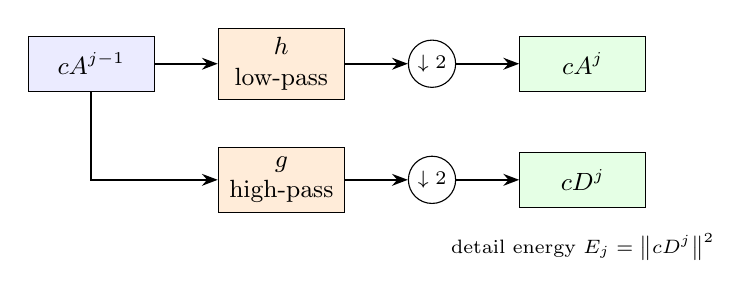
\begin{tikzpicture}[
  blk/.style={draw, minimum width=16mm, minimum height=7mm, font=\small, align=center},
  arr/.style={-{Stealth[length=2mm]}, thick},
  ds/.style={draw, circle, inner sep=1pt, font=\scriptsize, minimum size=6mm}
]
\node[blk, fill=blue!8] (in) {\(cA^{j-1}\)};
\node[blk, fill=orange!15, right=8mm of in] (lo) {\(h\)\\low-pass};
\node[blk, fill=orange!15, below=6mm of lo] (hi) {\(g\)\\high-pass};
\node[ds, right=8mm of lo] (ds1) {\(\downarrow 2\)};
\node[ds, right=8mm of hi] (ds2) {\(\downarrow 2\)};
\node[blk, fill=green!10, right=8mm of ds1] (a) {\(cA^{j}\)};
\node[blk, fill=green!10, right=8mm of ds2] (d) {\(cD^{j}\)};
\draw[arr] (in) -- (lo);
\draw[arr] (in.south) |- (hi.west);
\draw[arr] (lo) -- (ds1);
\draw[arr] (hi) -- (ds2);
\draw[arr] (ds1) -- (a);
\draw[arr] (ds2) -- (d);
\node[font=\scriptsize, align=left, below=2mm of d] {detail energy \(E_{j}=\norm{cD^{j}}^{2}\)};
\end{tikzpicture}
\caption{One step of the Mallat analysis bank. The detail coefficients at level \(j\) are the dyadic wavelet transform at scale \(2^{j}\).}
\label{fig:mallat}
\end{figure}

This exposition uses the Daubechies wavelet with four vanishing moments (db4) as the concrete mother wavelet.
The source does not name the mother wavelet.
Db4 is short, orthonormal, and has enough vanishing moments to annihilate a local cubic trend, which is the usual default when a monitoring study leaves the wavelet unnamed.
The analysis filters used to draw Figure~\ref{fig:energy} are the standard db4 pair.
A change to db6 or to a symlet moves the energy slightly between neighboring levels and does not change the definition of the map.
The level index, however, must be read against the sampling rate.
With \(f_{s}=10\,\mathrm{kHz}\), ideal dyadic half-bands place detail \(d_{j}\) roughly in
\begin{equation}
\Bigl(\frac{f_{s}}{2^{j+1}},\ \frac{f_{s}}{2^{j}}\Bigr).
\label{eq:bands}
\end{equation}
Detail \(d_{5}\) then occupies about \(156\)--\(312\,\mathrm{Hz}\), detail \(d_{6}\) about \(78\)--\(156\,\mathrm{Hz}\), and the shaft family \(\mathcal{F}\) itself, from \(8\,\mathrm{Hz}\) to \(96\,\mathrm{Hz}\), falls in \(d_{7}\), \(d_{8}\), and the final approximation.
The source figures identify \(d_{5}\) as the maximum-energy detail of the records they plot.
That observation is consistent with a structural or fluid resonance in the few-hundred-hertz band carrying more acceleration energy than the shaft tones, which is exactly what the factor \(-\omega^{2}\) in \eqref{eq:transfer} predicts.
The coefficient spectrum can still show shaft orders, because those orders modulate the resonant carrier, and because the spectrum the source plots is a spectrum of the selected detail's coefficient sequence with a frequency axis returned to hertz.
Both effects are part of the third block.

\begin{figure}[H]
\centering
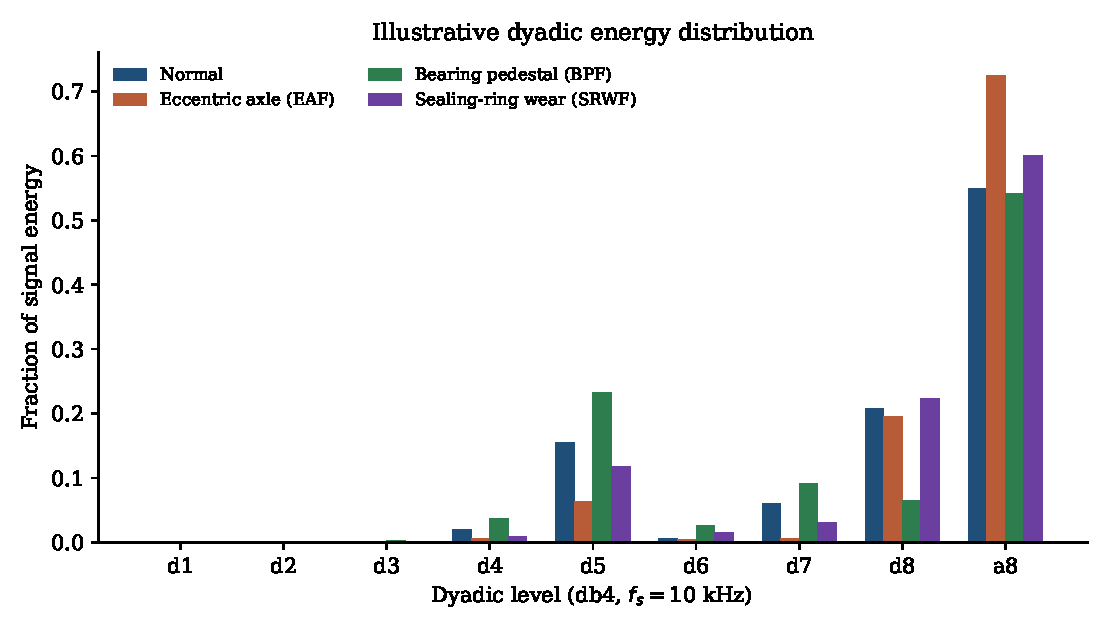
\includegraphics[width=0.92\textwidth]{wavelet_energy.pdf}
\caption{Fraction of energy by dyadic level for the illustrative signals, db4, eight levels. The bars are a partition of each synthetic record. They are not the energy table of the laboratory records, which the source publishes only as plots.}
\label{fig:energy}
\end{figure}

\subsection{Energy time-spectrum}

The source identifies the detail coefficients with the dyadic transform,
\begin{equation}
W_{f}(2^{j}, b)=cD^{j}[k],
\label{eq:identify}
\end{equation}
and defines the energy time-spectrum at scale \(2^{j}\) by the squared coefficients
\begin{equation}
E_{W_{f}(t)}(2^{j})=\abs{W_{f}(2^{j}, b)}^{2}=\abs{cD^{j}[k]}^{2}.
\label{eq:ets}
\end{equation}
Read as a function of the coefficient index, \eqref{eq:ets} is a time series, not a scalar.
It shows when, inside the record, scale \(2^{j}\) was loud.
A pedestal impact that occupies one millisecond raises \(E\) at the fine scales for that millisecond and leaves the rest of the series small.
A steady unbalance raises the coarse-scale series almost uniformly.
The scalar energy of the level, which decides the maximum, is the sum of the time series,
\begin{equation}
\mathcal{E}(2^{j})=\sum_{k}\abs{cD^{j}[k]}^{2}=\sum_{k} E_{W_{f}(t)}(2^{j})[k].
\label{eq:sumE}
\end{equation}
The maximum-energy level is the integer
\begin{equation}
k^{\star}\in\argmin_{1\le j\le J}\bigl(-\mathcal{E}(2^{j})\bigr),
\label{eq:kstar}
\end{equation}
that is, any level whose scalar energy is largest.
The source writes the assumption \(1\le k\le j\) for this index.
Ties are broken by choosing the finer level, so that a transient is preferred over a trend of equal energy.
On the source plots, \(k^{\star}=5\) for the displayed radial records of every state.
The map does not hard-code the number \(5\).
It recomputes \(k^{\star}\) for each record and each direction.
A fixed level would be a different method.

\subsection{Coefficient power spectrum of the maximum-energy level}

The third block reads the internal periodicity of the winning level.
The source forms the discrete Fourier transform of the energy time-series at \(k^{\star}\),
\begin{equation}
\widehat{E}_{W_{f}}(2^{k^{\star}})[\omega]
=\sum_{n=0}^{N_{c}-1} E_{W_{f}(t)}(2^{k^{\star}})[n]\,e^{-i\omega n/N_{c}},
\label{eq:fftE}
\end{equation}
and the power spectrum
\begin{equation}
E_{W_{p}}(\hat{\omega}, 2^{k^{\star}})
=\frac{1}{N_{c}}\left|\widehat{E}_{W_{f}}(2^{k^{\star}})[\omega]\right|^{2}.
\label{eq:cps}
\end{equation}
Here \(N_{c}\) is the length of the coefficient sequence at that level, which is about \(N/2^{k^{\star}}\) for an undecimated-free dyadic bank.
Equation \eqref{eq:cps} is the power spectrum of the energy envelope of the winning detail.
Peaks of an energy envelope sit at the rates that modulate the detail: a once-per-revolution modulation produces a line at \(f_{0}\) in this spectrum, and a twice-per-revolution looseness produces a line at \(\tfrac12 f_{0}\).

The plots in the source are labeled as the wavelet coefficient power spectrum of level \(d_{5}\) and are drawn with a horizontal axis in hertz from \(0\) to about \(110\,\mathrm{Hz}\), with visible lines at members of \(\mathcal{F}\).
Two implementations produce a plot of that shape.
The first is literal: transform \eqref{eq:ets} by \eqref{eq:fftE}, convert the coefficient-domain frequency \(\nu\) (cycles per coefficient) into hertz by
\begin{equation}
f=\nu\cdot\frac{f_{s}}{2^{k^{\star}}},
\label{eq:fmap}
\end{equation}
and read \eqref{eq:cps} on \(\mathcal{F}\).
The second forms the power spectrum of the detail coefficients themselves, without the square inside \eqref{eq:ets}, and uses the same frequency map.
The square emphasizes the strong instants of the detail and is the formula the source writes.
This exposition follows the written formula.
Amplitudes at the seven orders are then the samples of \eqref{eq:cps} nearest to each frequency in \(\mathcal{F}\),
\begin{equation}
p_{d}(\eta)=\left. E_{W_{p}}(\hat{\omega}, 2^{k^{\star}}) \right|_{f=\eta},
\qquad \eta\in\mathcal{F},\quad d\in\{r, t, a\}.
\label{eq:samples}
\end{equation}
If a line falls between bins, the bin of maximum power inside a window of half a shaft order is taken, so that a \(1\,\mathrm{Hz}\) speed drift does not zero the feature.
The source does not describe an interpolation rule.
The half-order window is a specification of this exposition, and it is narrower than the gap between adjacent members of \(\mathcal{F}\).

Figure~\ref{fig:spectra} shows the baseband power of the illustrative accelerations, normalized per state, with vertical lines at the same orders.
It is a spectrum of the raw synthetic signal, included so the harmonic emphasis is visible without the filter bank.
It is not a plot of \eqref{eq:cps}.

\begin{figure}[H]
\centering
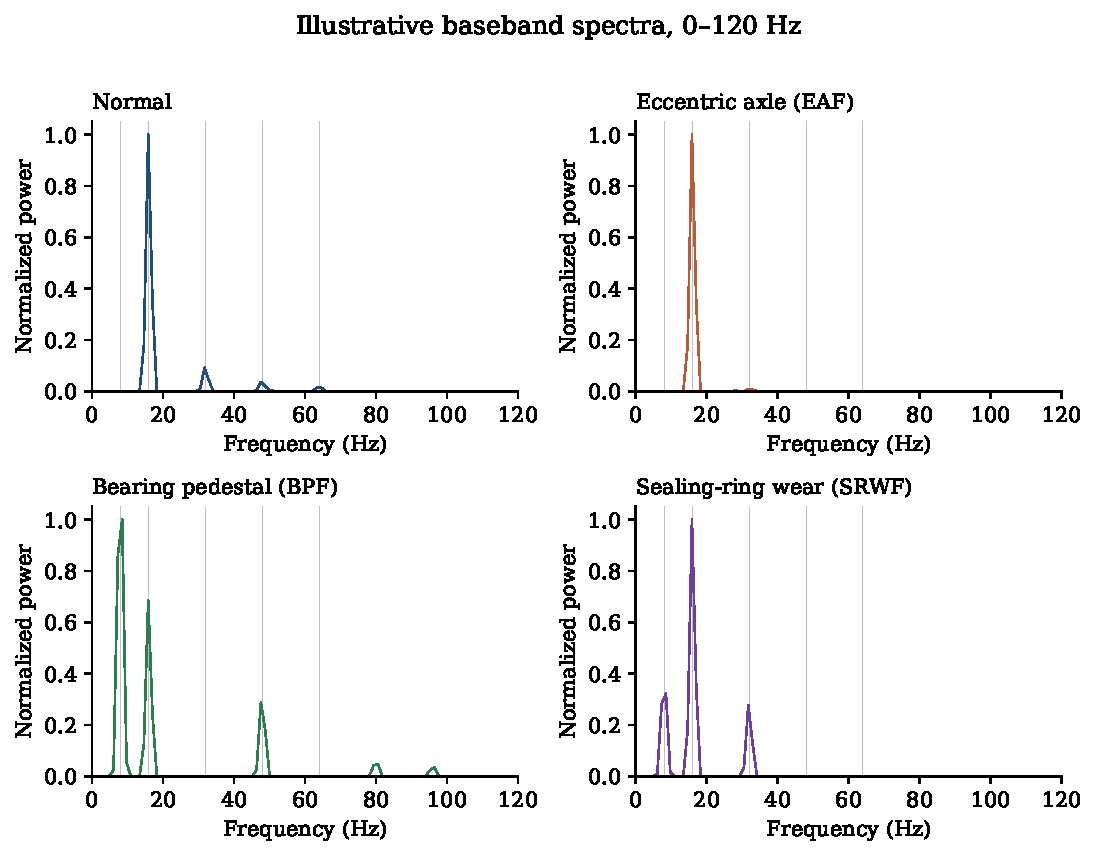
\includegraphics[width=0.94\textwidth]{spectra.pdf}
\caption{Normalized baseband spectra of the illustrative accelerations. Vertical lines mark \(8\), \(16\), \(32\), \(48\), and \(64\,\mathrm{Hz}\). Healthy energy favors \(f_{0}\) and its low harmonics; the eccentric state is dominated by \(f_{0}\); the pedestal and seal-wear states carry a stronger half-order.}
\label{fig:spectra}
\end{figure}

\subsection{Assembly of the twenty-two coordinates}

Collect the seven spectral samples on each axis and the radial severity:
\begin{equation}
\begin{aligned}
\vect{x}=\bigl(&
\mathrm{VIB}_{r},\\
&p_{t}(\tfrac12 f_{0}), p_{t}(f_{0}), \ldots, p_{t}(6f_{0}),\\
&p_{a}(\tfrac12 f_{0}), p_{a}(f_{0}), \ldots, p_{a}(6f_{0}),\\
&p_{r}(\tfrac12 f_{0}), p_{r}(f_{0}), \ldots, p_{r}(6f_{0})
\bigr)^{\!\top}\in\R^{22}.
\end{aligned}
\label{eq:x22}
\end{equation}
The order of the blocks is a convention.
Training and testing must use the same convention, because the SVM kernel compares coordinates by index.
The source's reading of its own Figure~9 fixes the meaning of the blocks even without a written index map.
In the healthy state the tangential amplitudes exceed the axial and the radial ones, and the tangential maximum lies at \(f_{0}\).
Under the eccentric axle the tangential maximum rises from \(1.683\times 10^{-3}\) to \(3.322\times 10^{-3}\) in the units of that figure, the axial energy spreads from \(f_{0}\) toward \(\tfrac12 f_{0}\), and the radial maximum rises from \(4.574\times 10^{-4}\) to \(2.492\times 10^{-3}\).
Under the pedestal fault the tangential maximum rises further, to \(4.701\times 10^{-3}\), and it sits at \(\tfrac12 f_{0}\) rather than at \(f_{0}\); axial energy grows at \(5f_{0}\) and \(6f_{0}\); radial energy shifts from \(f_{0}\) toward \(\tfrac12 f_{0}\), \(3f_{0}\), and \(4f_{0}\).
Under sealing-ring wear the tangential amplitudes are again the largest, with emphasis at \(f_{0}\), \(\tfrac12 f_{0}\), and \(2f_{0}\), and the axial and radial intensities fall between the eccentric and the pedestal cases.
Those sentences are the specification of what \(\Phi\) is supposed to make linearly visible.
A correct implementation is one in which a scatter of the \(22\)-vectors reproduces this pattern.

\subsection{Normalization}

Coordinates of \(\vect{x}\) do not share a unit.
Severity is in millimetres per second and has magnitude near \(1\).
A coefficient power sample is a squared spectral density of a squared wavelet coefficient, and the published tangential peaks lie near \(10^{-3}\).
Left unscaled, the Euclidean distances inside the radial kernel are severity distances, and the twenty-one spectral coordinates are ignored.
The source states that training and testing vectors are normalized before classification in order to speed convergence.
It does not state the map.
This exposition uses an affine map to the unit interval, fit on the training sample only,
\begin{equation}
\tilde{x}^{(j)}=\frac{x^{(j)}-u^{(j)}}{v^{(j)}-u^{(j)}},
\qquad
u^{(j)}=\min_{i\in\mathrm{train}} x_{i}^{(j)},
\quad
v^{(j)}=\max_{i\in\mathrm{train}} x_{i}^{(j)}.
\label{eq:norm}
\end{equation}
The same \(u^{(j)}\) and \(v^{(j)}\) are applied to the test vectors.
Refitting the range on the test set would leak the test distribution into the feature and would inflate the estimate in Chapter~\ref{ch:estimation}.
A coordinate with \(v^{(j)}=u^{(j)}\) is dropped; on this rig none of the twenty-two is constant.
A \(z\)-score is an acceptable alternative and is not the map used in the formulae below.

\subsection{The feature procedure}

The map \(\Phi\), ready to implement, is the following procedure.
\begin{enumerate}
\item From each acceleration axis, form the velocity series by the chosen integrator and compute one radial severity by \eqref{eq:vibdisc}.
\item For each axis, run \(J=8\) steps of \eqref{eq:mallat} with the db4 filters.
Compute the scalar energies \eqref{eq:sumE} and the winning index \(k^{\star}\) by \eqref{eq:kstar}.
\item Form the energy time-series \eqref{eq:ets} at level \(k^{\star}\), its transform \eqref{eq:fftE}, and the power \eqref{eq:cps}.
Sample the seven orders by \eqref{eq:samples}.
\item Concatenate by \eqref{eq:x22}.
\item Apply \eqref{eq:norm} with ranges stored from the training fold.
\end{enumerate}
The cost is linear in \(N\) for the filter bank and \(O(N_{c}\log N_{c})\) for the single transform of the winning level.
At \(N=8192\) this cost is negligible beside the cost of the SVM trainings inside the parameter search.
The map contains no iterative optimization and no random seed.
Given the filter, the integrator, and the tie break, \(\Phi\) is a function.

\subsection{How the four states separate inside the map}

A short mechanical reading says what a later classifier is asked to finish.
Healthy running puts a moderate severity next to a tangential spectrum peaked at \(16\,\mathrm{Hz}\), with smaller lines at \(32\), \(48\), and \(64\,\mathrm{Hz}\) and a supply artifact at \(50\,\mathrm{Hz}\) that the order sampler, aimed at \(48\,\mathrm{Hz}\), is narrow enough to miss.
Eccentric axle multiplies the severity by about three and multiplies the tangential \(f_{0}\) sample by about two, which is the stationary signature of a larger \(me\Omega^{2}\) in \eqref{eq:rotor}.
Bearing-pedestal fault leaves the severity almost unchanged and moves the tangential peak from \(16\,\mathrm{Hz}\) to \(8\,\mathrm{Hz}\), which is the spectral form of a stiffness that repeats every two revolutions, and it raises high-order axial energy that the source attributes to flow-induced vibration and to component natural frequencies.
Sealing-ring wear raises the severity to \(1.70\,\mathrm{mm/s}\) and emphasizes \(\tfrac12 f_{0}\) together with \(2f_{0}\), which is the hydraulic leakage writing on the orbit twice per turn as well as once every two turns.
These four patterns are not orthogonal, and the pedestal pattern is the least stable of them because resonance and site interference share the bands the high orders occupy.
The classifier of the next section is trained to draw the boundaries that these patterns only suggest.

\begin{figure}[H]
\centering
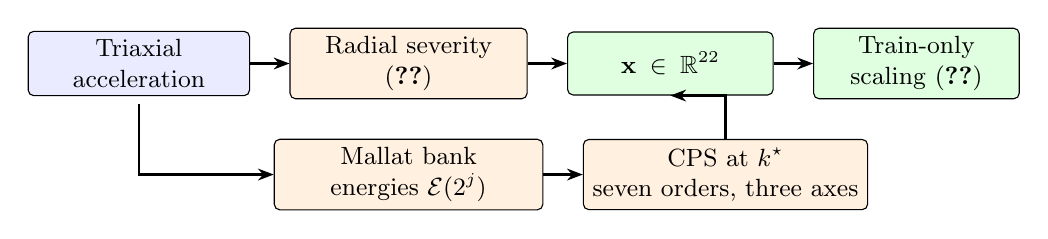
\begin{tikzpicture}[
  box/.style={draw, rounded corners=2pt, align=center, font=\small, inner sep=3pt, minimum height=8mm},
  arr/.style={-{Stealth[length=2mm]}, thick}
]
\node[box, fill=blue!8, text width=26mm] (a) {Triaxial\\acceleration};
\node[box, fill=orange!12, text width=28mm, right=5mm of a] (v) {Radial severity\\\eqref{eq:vibdisc}};
\node[box, fill=orange!12, text width=32mm, below=5mm of v] (w) {Mallat bank\\energies \(\mathcal{E}(2^{j})\)};
\node[box, fill=orange!12, text width=34mm, right=5mm of w] (c) {CPS at \(k^{\star}\)\\seven orders, three axes};
\node[box, fill=green!12, text width=24mm, right=5mm of v] (x) {\(\vect{x}\in\R^{22}\)};
\node[box, fill=green!12, text width=24mm, right=5mm of x] (n) {Train-only\\scaling \eqref{eq:norm}};
\draw[arr] (a) -- (v);
\draw[arr] (a.south) ++(0,-1mm) |- (w.west);
\draw[arr] (w) -- (c);
\draw[arr] (v) -- (x);
\draw[arr] (c.north) |- (x.south);
\draw[arr] (x) -- (n);
\end{tikzpicture}
\caption{Data flow of the VWC map. Severity and the spectral block meet only at the concatenation.}
\label{fig:vwcflow}
\end{figure}

\section{Technology two: the MSFLA-SVM classifier}
\label{sec:svm}

\subsection{Hard margin}

The second technology starts from a binary labeled sample, because the multiclass pump problem is reduced to binary problems below.
Let
\begin{equation}
\mathcal{T}=\bigl\{(\vect{x}_{i}, y_{i})\bigr\}_{i=1}^{n},
\qquad \vect{x}_{i}\in\R^{d},\quad y_{i}\in\{+1,-1\}.
\label{eq:binset}
\end{equation}
A linear classifier is a pair \((\vect{w}, b)\) and the rule \(\sgn(\vect{w}^{\top}\vect{x}+b)\).
Among all pairs that separate \(\mathcal{T}\), the hard-margin SVM chooses the pair whose slab
\begin{equation}
\bigl\{\vect{x}:\ \abs{\vect{w}^{\top}\vect{x}+b}\le 1\bigr\}
\label{eq:slab}
\end{equation}
is as thick as possible.
The Euclidean thickness of the slab is \(2/\norm{\vect{w}}\).
Maximizing the thickness is the same problem as
\begin{equation}
\min_{\vect{w}, b}\ \frac{1}{2}\norm{\vect{w}}^{2}
\quad\text{subject to}\quad
y_{i}(\vect{w}^{\top}\vect{x}_{i}+b)\ge 1,
\quad i=1,\ldots,n.
\label{eq:hard}
\end{equation}
The factor one half is traditional and makes the derivative equal to \(\vect{w}\).
Points that lie on the boundary of the slab are the support vectors.
They alone determine \(\vect{w}\).
Moving a correctly classified point that sits strictly outside the slab does not change the solution, which is the geometric reason a small sample can still determine a stable rule: most of the sample is allowed to be absent.

\begin{figure}[H]
\centering
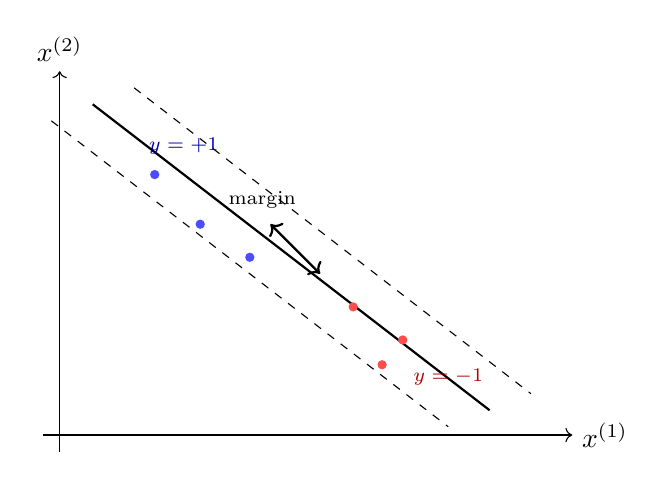
\begin{tikzpicture}[scale=1.05]
  \draw[->] (-0.2,0) -- (6.2,0) node[right] {\(x^{(1)}\)};
  \draw[->] (0,-0.2) -- (0,4.4) node[above] {\(x^{(2)}\)};
  \draw[thick] (0.4,4.0) -- (5.2,0.3);
  \draw[dashed] (0.9,4.2) -- (5.7,0.5);
  \draw[dashed] (-0.1,3.8) -- (4.7,0.1);
  \fill[blue!70] (1.15,3.15) circle (1.6pt);
  \fill[blue!70] (1.7,2.55) circle (1.6pt);
  \fill[blue!70] (2.3,2.15) circle (1.6pt);
  \fill[red!70] (3.55,1.55) circle (1.6pt);
  \fill[red!70] (4.15,1.15) circle (1.6pt);
  \fill[red!70] (3.9,0.85) circle (1.6pt);
  \draw[<->, thick] (2.55,2.55) -- (3.15,1.95);
  \node[font=\scriptsize] at (2.45,2.85) {margin};
  \node[font=\scriptsize, blue!70!black] at (1.5,3.5) {\(y=+1\)};
  \node[font=\scriptsize, red!70!black] at (4.7,0.7) {\(y=-1\)};
\end{tikzpicture}
\caption{Hard-margin geometry in a feature plane. The solid line is the decision boundary. The dashed lines bound the slab. Only points on the dashed lines are support vectors.}
\label{fig:margin}
\end{figure}

\subsection{Soft margin and the dual}

Pump features overlap, so the constraints of \eqref{eq:hard} can be empty.
The soft-margin problem introduces a slack \(\xi_{i}\ge 0\) for each training point and a penalty \(C>0\) on the sum of slacks,
\begin{equation}
\min_{\vect{w}, b, \xi}\ 
\frac{1}{2}\norm{\vect{w}}^{2}+C\sum_{i=1}^{n}\xi_{i}
\quad\text{subject to}\quad
y_{i}(\vect{w}^{\top}\vect{x}_{i}+b)\ge 1-\xi_{i},\quad \xi_{i}\ge 0.
\label{eq:soft}
\end{equation}
A small \(C\) permits a wide margin with many slacks and under-fits the four states.
A large \(C\) forces the slacks toward zero and can memorize the \(180\) training vectors.
This is the first of the two numbers the frog search has to set.
The Lagrangian of \eqref{eq:soft} with multipliers \(\alpha_{i}\ge 0\) for the margin inequalities and \(\mu_{i}\ge 0\) for the slack inequalities has a saddle point at which \(\vect{w}=\sum_{i}\alpha_{i} y_{i}\vect{x}_{i}\) and \(\sum_{i}\alpha_{i} y_{i}=0\).
Eliminating \(\vect{w}\), \(b\), and \(\xi\) produces the dual quadratic program that the source writes in kernel form.
In the linear case it is
\begin{equation}
\begin{aligned}
\max_{\alpha}\quad
&-\frac{1}{2}\sum_{i=1}^{n}\sum_{j=1}^{n} y_{i} y_{j}\alpha_{i}\alpha_{j}\,\vect{x}_{i}^{\top}\vect{x}_{j}
+\sum_{j=1}^{n}\alpha_{j}\\
\text{subject to}\quad
&\sum_{i=1}^{n} y_{i}\alpha_{i}=0,
\qquad 0\le \alpha_{i}\le C.
\end{aligned}
\label{eq:dual}
\end{equation}
The box constraint \(0\le\alpha_{i}\le C\) is the algebraic face of the penalty.
A point with \(\alpha_{i}=0\) is outside the slab and does not appear in \(\vect{w}\).
A point with \(0<\alpha_{i}<C\) lies on the margin boundary and is a free support vector.
A point with \(\alpha_{i}=C\) lies inside the slab or on the wrong side and is a bound support vector.
The decision rule, once any free support vector \(\vect{x}_{j}\) has been used to recover the threshold, is
\begin{equation}
f(\vect{x})=\sgn\Bigl(\sum_{i=1}^{n}\alpha_{i} y_{i}\,\vect{x}_{i}^{\top}\vect{x}+b\Bigr),
\label{eq:declin}
\end{equation}
\begin{equation}
b=y_{j}\Bigl(1-\frac{\alpha_{j}}{C}\Bigr)-\sum_{i=1}^{n} y_{i}\alpha_{i}\,\vect{x}_{i}^{\top}\vect{x}_{j},
\label{eq:bias}
\end{equation}
which is the linear special case of the source formulae.
Sequential minimal optimization solves \eqref{eq:dual} by optimizing two multipliers at a time and keeping the equality constraint satisfied.
The solver is deterministic given the data, \(C\), and the kernel.
All of the randomness in MSFLA-SVM sits in the outer search, not in the quadratic program.

\subsection{The radial kernel}

Pump classes are not linearly separable in \(\R^{22}\) after the normalization \eqref{eq:norm}.
A feature map \(\Psi\) into a Hilbert space \(\mathcal{H}\) restores a linear problem in \(\mathcal{H}\) provided the inner products \(\langle\Psi(\vect{x}),\Psi(\vect{x}')\rangle_{\mathcal{H}}\) can be evaluated.
Mercer's theorem says that a continuous symmetric function \(K\) that is positive definite is such an inner product for some \(\Psi\).
The radial basis used by the source,
\begin{equation}
K(\vect{x}, \vect{x}')
=\exp\Bigl(-\frac{\norm{\vect{x}-\vect{x}'}^{2}}{2\sigma^{2}}\Bigr)
=\exp\bigl(-g\,\norm{\vect{x}-\vect{x}'}^{2}\bigr),
\label{eq:rbf}
\end{equation}
is positive definite for every \(\sigma>0\).
The second writing defines the kernel parameter \(g=1/(2\sigma^{2})\) that the search actually stores.
A large \(g\) makes \(K\) decay in a small neighborhood of each training point: the decision surface can weave among the \(180\) vectors and the risk of over-fit rises.
A small \(g\) makes \(K\) almost constant on the unit cube: the surface is nearly linear and the risk of under-fit rises.
The source notes that \(\sigma\), or equivalently \(g\), balances the influence of \(C\).
The pair \((C, g)\) is the whole continuous degree of freedom of the classifier.
Substituting \(K\) for the inner product in \eqref{eq:dual} gives the program the source states,
\begin{equation}
\begin{aligned}
\min_{\alpha}\quad
&\frac{1}{2}\sum_{i=1}^{n}\sum_{j=1}^{n}
y_{i} y_{j}\alpha_{i}\alpha_{j}
\Bigl(K(\vect{x}_{i}, \vect{x}_{j})+\frac{1}{C}\delta_{ij}\Bigr)
-\sum_{j=1}^{n}\alpha_{j}\\
\text{subject to}\quad
&\sum_{i=1}^{n} y_{i}\alpha_{i}=0,\qquad \alpha_{i}\ge 0,
\end{aligned}
\label{eq:dualk}
\end{equation}
where the diagonal term \(C^{-1}\delta_{ij}\) is the source's way of writing the soft-margin quadratic, and the decision function is
\begin{equation}
f(\vect{x})=\sgn\Bigl(\sum_{i=1}^{n}\alpha_{i}^{\star} y_{i} K(\vect{x}, \vect{x}_{i})+b^{\star}\Bigr).
\label{eq:decf}
\end{equation}
The threshold \(b^{\star}\) is computed from any multiplier strictly between \(0\) and \(C\), by the kernel form of \eqref{eq:bias}.

\subsection{Four states from binary machines}

The label set of the pump is
\begin{equation}
\mathcal{Y}=\{\text{normal},\ \text{EAF},\ \text{BPF},\ \text{SRWF}\},
\label{eq:Y}
\end{equation}
not a pair.
This exposition reduces \(\mathcal{Y}\) by the one-versus-one scheme.
Each pair of states trains one binary machine, which produces
\begin{equation}
\binom{4}{2}=6
\label{eq:ovo}
\end{equation}
radial SVMs.
A test vector is labeled by the state that wins the most of the six votes.
Ties are broken by the signed sum of the six decision functions after each function has been oriented toward its positive class.
One-versus-rest, with four machines, is the main alternative.
It trains each machine on a more unbalanced binary problem, because the negative class then contains three states.
The source does not name the reduction.
One-versus-one is the specification here because each binary problem then has \(90\) training vectors, \(45\) per state, which matches the per-state training count the source publishes, and because it is the default reduction of the usual SVM solver.
The search for \((C, g)\) is shared: one pair is used for all six machines, and the fitness of that pair is the cross-validated accuracy of the voted label, not the accuracy of a single binary machine.
Searching six independent pairs would multiply the capacity of the outer loop by six and, on \(180\) vectors, would over-fit the folds.

\subsection{Cross-validated fitness}

A frog is a candidate pair \(\vect{z}=(C, g)\) with \(C>0\) and \(g>0\).
The search works in logarithmic coordinates
\begin{equation}
\vect{u}=(\log_{10} C,\ \log_{10} g),
\label{eq:logcoord}
\end{equation}
so that a leap of fixed length means the same factor at \(C=1\) and at \(C=10^{3}\).
The box of this exposition is
\begin{equation}
\log_{10} C\in[-1, 3],\qquad \log_{10} g\in[-3, 1],
\label{eq:box}
\end{equation}
which covers penalties from \(0.1\) to \(1000\) and kernel parameters over four decades around the scale of the unit-cube features.
The source does not publish a box.
Equation \eqref{eq:box} is a specification, chosen to match the range a careful grid search would have covered, and every leap is projected back into the box by truncation.

The fitness of \(\vect{u}\) is a stratified \(K\)-fold accuracy on the training set.
With \(n=180\) and four classes, \(K=5\) gives folds of \(36\) vectors, nine from each state.
For each fold the six binary machines are trained on the complement, the fold is labeled by vote, and the accuracy is the fraction of correct labels.
The fitness is the mean of the five accuracies,
\begin{equation}
F(\vect{u})=\frac{1}{K}\sum_{k=1}^{K}\mathrm{Acc}\bigl(\mathcal{T}\setminus\mathcal{T}_{k};\ \mathcal{T}_{k};\ \vect{u}\bigr).
\label{eq:fitness}
\end{equation}
\(F\) is a step function.
It changes only when a leap moves a training vector across a margin.
Gradient methods are a poor match to it, which is why a derivative-free leap is the right outer loop.
The value of \(F\) is the only information a frog receives.
In particular the search never sees the test set.
The numbers in Chapter~\ref{ch:estimation} are computed after the search has returned its best \(\vect{u}\), by retraining on all \(180\) vectors and labeling the \(60\).

\subsection{The unmodified shuffled frog-leaping search}

The unmodified search is the baseline called SFLA-SVM.
A population of \(N_{f}\) frogs
\begin{equation}
\vect{U}_{i}=(\vect{u}_{i,1}, \ldots, \vect{u}_{i,d}),\qquad d=2,
\label{eq:frogs}
\end{equation}
is drawn uniformly in the box \eqref{eq:box}.
The source's dimension \(d\) is the dimension of a frog, which is two, not the feature dimension \(22\).
Fitness \(F(\vect{U}_{i})\) is evaluated by \eqref{eq:fitness}.
The frogs are sorted so that \(F(\vect{U}_{1})\ge F(\vect{U}_{2})\ge\cdots\), and they are dealt into \(M\) memeplexes of \(P\) frogs with \(N_{f}=M P\).
Frog \(i\) in the sorted list goes to memeplex
\begin{equation}
z=(i-1)\bmod M,
\label{eq:deal}
\end{equation}
which is the source rule \(z=i\bmod M\) up to the indexing of the first frog.
Dealing by rank, rather than by chopping the sorted list into \(M\) contiguous blocks, puts a high-fitness frog in every memeplex.
Each memeplex then has a local best frog \(\vect{F}_{b}\), the whole population has a global best frog \(\vect{F}_{g}\), and each memeplex has a worst frog \(\vect{F}_{w}\).

The local leap tries to improve \(\vect{F}_{w}\) by moving it toward \(\vect{F}_{b}\),
\begin{equation}
\begin{aligned}
\vect{D}&=\mathrm{rand}(0,1)\cdot(\vect{F}_{b}-\vect{F}_{w}),\\
\vect{F}_{w}^{\mathrm{new}}&=\mathrm{clip}\bigl(\vect{F}_{w}+\vect{D};\ \pm D_{\max}\bigr),
\end{aligned}
\label{eq:leapb}
\end{equation}
where the clip enforces both the box and a maximum step length \(D_{\max}\) on each coordinate.
If \(F(\vect{F}_{w}^{\mathrm{new}})\) is not strictly better than \(F(\vect{F}_{w})\), the same leap is repeated with \(\vect{F}_{g}\) in place of \(\vect{F}_{b}\).
If that also fails, \(\vect{F}_{w}\) is replaced by a uniform random frog in the box.
Each memeplex repeats its local improvement a fixed number of times.
All memeplexes are then poured back into one population, sorted, and dealt again.
The shuffle is the only communication between memeplexes, apart from the shared use of \(\vect{F}_{g}\).
The loop stops at a maximum number of shuffles or when \(F(\vect{F}_{g})\) has met a prescribed accuracy.

The two defects of this loop are visible from the formulae.
The leap uses \(\vect{F}_{b}\) and \(\vect{F}_{g}\) only in sequence, and only the second if the first has already failed, so a frog that can gain from a combination of the two leaders never sees the combination.
And the random replacement ignores \(\vect{F}_{w}\) entirely.
Late in the run, when most frogs lie near one another, both defects reduce diversity: the sequential leap copies the leaders, and the random replacement is rare only when leaps succeed, which is when the population has already collapsed.

\subsection{Distance-weighted update of the worst frog}

The modified search changes the leap and the failure case.
Inside memeplex \(z\), write \(\vect{X}_{h}\) for the position of its \(h\)-th frog and define the memeplex center by the coordinate-wise mean
\begin{equation}
\vect{U}_{z,c}=\frac{1}{P}\sum_{h=1}^{P}\vect{X}_{h}.
\label{eq:center}
\end{equation}
The distance the source uses between two frogs \(i\) and \(j\) is not a plain Euclidean distance of their positions.
It adds the distance of the centers of the memeplexes that hold them,
\begin{equation}
\mathrm{FFdist}(i, j)
=\sqrt{\sum_{t=1}^{d}\bigl(U_{i,t}-U_{j,t}\bigr)^{2}
+\norm{\vect{U}_{i,c}-\vect{U}_{j,c}}^{2}}.
\label{eq:ffdist}
\end{equation}
A frog is therefore far from another frog either because its parameters differ or because it sits in a memeplex whose center differs.
The second term keeps two memeplexes that have drifted apart from treating their members as neighbors merely because two of the members happen to be close.
Let \(S\) be the index of the global best frog, and define
\begin{align}
D_{\max}^{g}&=\max_{i\neq S}\ \mathrm{FFdist}(i, S),&
D_{\min}^{g}&=\min_{i\neq S}\ \mathrm{FFdist}(i, S).
\label{eq:dminmax}
\end{align}
The learning weight on the global leader, for a frog \(i\) that is about to leap, is the normalized distance
\begin{equation}
q_{i}=\frac{\mathrm{FFdist}(i, S)-D_{\min}^{g}}{D_{\max}^{g}-D_{\min}^{g}},
\qquad h_{i}=1-q_{i}.
\label{eq:qh}
\end{equation}
When the denominator vanishes, every frog is at the same distance from the leader and the weights are set to \(h_{i}=q_{i}=\tfrac12\).
By construction \(h_{i}+q_{i}=1\) and both weights lie in \([0,1]\).
A frog close to the global best receives a small \(q_{i}\) and a large \(h_{i}\): its leap is mostly toward the local best, which is a fine adjustment.
A frog far from the global best receives a large \(q_{i}\): its leap is mostly toward the global best, which pulls outliers inward without waiting for the local leap to fail.
The modified step is the single update
\begin{equation}
\begin{aligned}
\vect{D}_{i}
&=h_{i}\,\mathrm{rand}(0,1)\,(\vect{F}_{b}-\vect{F}_{w})
+q_{i}\,\mathrm{rand}(0,1)\,(\vect{F}_{g}-\vect{F}_{w}),\\
\vect{F}_{w}^{\mathrm{new}}
&=\mathrm{clip}\bigl(\vect{F}_{w}+\vect{D}_{i};\ \pm D_{\max}\bigr).
\end{aligned}
\label{eq:msfla}
\end{equation}
The two \(\mathrm{rand}(0,1)\) draws are independent.
Equation \eqref{eq:msfla} replaces the cascade \eqref{eq:leapb}.
There is no second chance with a different leader, because both leaders are already in the step.
If the new fitness is strictly better, \(\vect{F}_{w}^{\mathrm{new}}\) replaces \(\vect{F}_{w}\).

\begin{figure}[H]
\centering
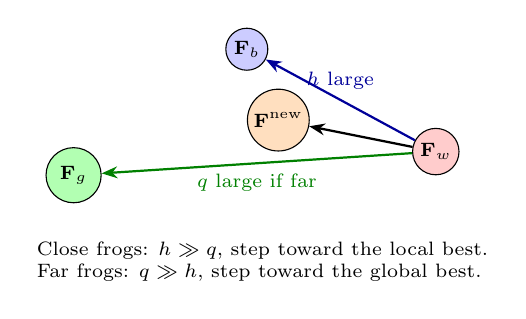
\begin{tikzpicture}[
  frog/.style={circle, draw, inner sep=1.5pt, font=\scriptsize},
  arr/.style={-{Stealth[length=2mm]}, thick}
]
  \node[frog, fill=green!30, minimum size=7mm] (g) at (0,0) {\(\vect{F}_{g}\)};
  \node[frog, fill=blue!20] (b) at (2.2,1.6) {\(\vect{F}_{b}\)};
  \node[frog, fill=red!20] (w) at (4.6,0.3) {\(\vect{F}_{w}\)};
  \node[frog, fill=orange!25] (n) at (2.6,0.7) {\(\vect{F}^{\mathrm{new}}\)};
  \draw[arr, blue!60!black] (w) -- (b) node[midway, above, font=\scriptsize] {\(h\) large};
  \draw[arr, green!50!black] (w) -- (g) node[midway, below, font=\scriptsize] {\(q\) large if far};
  \draw[arr] (w) -- (n);
  \node[font=\scriptsize, align=left] at (2.4,-1.1) {Close frogs: \(h\gg q\), step toward the local best.\\Far frogs: \(q\gg h\), step toward the global best.};
\end{tikzpicture}
\caption{The modified leap. The new position of the worst frog is a convex combination, with random contractions, of the step toward the local best and the step toward the global best. The weights depend on distance to the global best.}
\label{fig:leap}
\end{figure}

\subsection{Gaussian mutation when the leap fails}

If \(F(\vect{F}_{w}^{\mathrm{new}})\le F(\vect{F}_{w})\), the unmodified search draws a new frog uniformly in the box.
The modified search perturbs the current worst frog by an isotropic Gaussian factor,
\begin{equation}
\vect{F}_{w}^{\mathrm{mut}}
=\mathrm{clip}\bigl(\vect{F}_{w}+\vect{F}_{w}\odot\boldsymbol{\varepsilon}\bigr),
\qquad
\boldsymbol{\varepsilon}\sim\mathcal{N}(\vect{0}, \vect{I}),
\label{eq:gauss}
\end{equation}
where \(\odot\) is coordinate-wise multiplication and the clip returns the result to the box \eqref{eq:box}.
Because the coordinates of \(\vect{F}_{w}\) are logarithms of \(C\) and \(g\), adding a multiple of the coordinate itself is a multiplicative perturbation in the original parameters:
a coordinate \(u\) becomes \(u(1+\varepsilon)\).
A draw \(\varepsilon=-1\) would send the coordinate through zero; the box truncation stops that case.
The perturbation is local in the logarithmic chart whenever \(\boldsymbol{\varepsilon}\) is order one, and it is still able to leave a shallow local maximum, which is the reason for using a unit normal rather than a very small one.
The mutated frog replaces \(\vect{F}_{w}\) whether or not its fitness improves.
That acceptance of a worse mutant is what restores diversity after a failed leap.
It is also the reason the mutant must stay in a neighborhood of \(\vect{F}_{w}\): a worse mutant thrown to the other end of the box would be the blind restart again.
The source writes the mutation as \(F_{w}+F_{w}\cdot N(0,1)\), which is \eqref{eq:gauss} before the clip.
The clip is part of this exposition because an unconstrained Gaussian step on a bad frog can exit the box in one generation.

\subsection{The modified procedure as a whole}

The full outer loop, with the inner SVM treated as a subroutine that returns \(F\), is the following.
\begin{enumerate}
\item Draw \(N_{f}=M P\) frogs uniformly in the box \eqref{eq:box}.
Evaluate \(F\) by \eqref{eq:fitness}.
\item Sort the frogs by decreasing fitness and deal them into \(M\) memeplexes by \eqref{eq:deal}.
\item For each memeplex, for a prescribed number of local steps: identify \(\vect{F}_{b}\), \(\vect{F}_{w}\), and the global \(\vect{F}_{g}\); compute centers and the weights \eqref{eq:qh}; propose \(\vect{F}_{w}^{\mathrm{new}}\) by \eqref{eq:msfla}; if the fitness improves, accept it; otherwise replace \(\vect{F}_{w}\) by the mutant \eqref{eq:gauss}.
\item Shuffle all memeplexes into one population.
\item If the shuffle budget is exhausted, or if \(F(\vect{F}_{g})\) has reached the prescribed accuracy, stop and return \(\vect{F}_{g}\).
Otherwise return to step 2.
\item Retrain the six binary SVMs on all \(180\) training vectors at the returned \((C, g)\), and label the test vectors by vote.
\end{enumerate}
Population size, memeplex count, local-step count, shuffle budget, and \(D_{\max}\) are not printed in the source study.
They are parameters of the search, not of the SVM.
This exposition does not assign them numerical values disguised as the experimental settings.
What the published estimate in Chapter~\ref{ch:estimation} supports is the whole procedure as the source ran it, not a particular population size reconstructed after the fact.
An implementation that needs numbers can start from a small memetic configuration, \(M=5\), \(P=10\), ten local steps, and thirty shuffles, and check that the cross-validated fitness has flattened.
Those starting values are a suggestion for software, not a claim about the 2019 run.

\subsection{Relation to the other outer loops}

The four classifiers in the published comparison share the VWC vector and differ in the map from that vector to a label.
The backpropagation network fits \eqref{eq:bpnn} by gradients and has no \((C, g)\).
ACROA-SVM fits the same dual \eqref{eq:dualk} and proposes \((C, g)\) by chemical-reaction moves: combinations of candidates, decompositions, and intermolecular collisions, accepted by a reaction criterion.
SFLA-SVM proposes \((C, g)\) by the cascade \eqref{eq:leapb} and by random replacement.
MSFLA-SVM proposes \((C, g)\) by \eqref{eq:msfla} and \eqref{eq:gauss}.
Any difference in the tables of Chapter~\ref{ch:estimation} is therefore a difference of inductive bias and of search, on a common feature.
It is not a difference of sensors or of labels.

A useful way to see the modified leap is to write the expected step, conditional on the current frogs, ignoring the clip.
Because each \(\mathrm{rand}(0,1)\) has mean one half,
\begin{equation}
\E[\vect{D}_{i}\mid \text{leaders}]
=\frac{h_{i}}{2}(\vect{F}_{b}-\vect{F}_{w})+\frac{q_{i}}{2}(\vect{F}_{g}-\vect{F}_{w}).
\label{eq:expect}
\end{equation}
The expected new position is an affine combination of \(\vect{F}_{w}\), \(\vect{F}_{b}\), and \(\vect{F}_{g}\) whose weights on the two leaders sum to one half.
The unmodified cascade has a different expectation: it moves toward \(\vect{F}_{b}\) alone with probability one on the first try, and toward \(\vect{F}_{g}\) only on failure.
Equation \eqref{eq:expect} is biased toward exploration exactly when \(q_{i}\) is large, which is when \(\mathrm{FFdist}(i, S)\) is large.
That is the diversity mechanism, expressed as a conditional expectation rather than as a slogan.
The Gaussian mutant adds a zero-mean perturbation on the failure event, so it does not change \eqref{eq:expect} on the event that the leap succeeds, and it prevents the failure event from sampling the box uniformly.

\subsection{Numerical safeguards}

A few safeguards keep the procedure inside the theory that justifies it.
The kernel matrix is positive definite up to rounding; a practical solver adds a ridge of size about \(10^{-8}\) to the diagonal, which is a negligible shift of \(C^{-1}\) inside the box \eqref{eq:box}.
Features enter only after \eqref{eq:norm}, so a change of engineering unit cannot masquerade as a change of \(g\).
Fitness is computed on stratified folds, so a frog cannot score perfectly by ignoring the pedestal class, which has the same training count as the others but is harder.
The test set is touched once, after the return of \(\vect{F}_{g}\).
Repeating the search from several random populations and keeping the best training fitness would be a further outer loop and would require a fresh test set to stay honest.
The published estimate is the result of the search the source ran, reported once.

\begin{figure}[H]
\centering
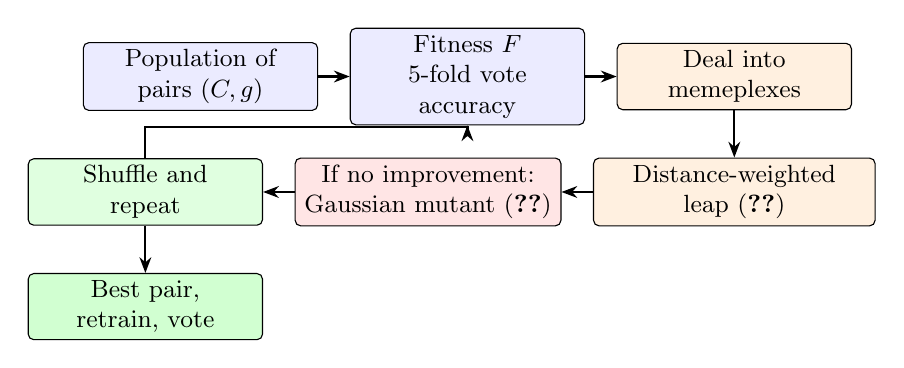
\begin{tikzpicture}[
  box/.style={draw, rounded corners=2pt, align=center, font=\small, inner sep=2.5pt, minimum height=8mm},
  arr/.style={-{Stealth[length=2mm]}, thick}
]
\node[box, fill=blue!8, text width=28mm] (pop) {Population of\\pairs \((C, g)\)};
\node[box, fill=blue!8, text width=28mm, right=4mm of pop] (fit) {Fitness \(F\)\\5-fold vote accuracy};
\node[box, fill=orange!12, text width=28mm, right=4mm of fit] (deal) {Deal into\\memeplexes};
\node[box, fill=orange!12, text width=34mm, below=6mm of deal] (leap) {Distance-weighted\\leap \eqref{eq:msfla}};
\node[box, fill=red!10, text width=32mm, left=4mm of leap] (mut) {If no improvement:\\Gaussian mutant \eqref{eq:gauss}};
\node[box, fill=green!12, text width=28mm, left=4mm of mut] (shuf) {Shuffle and\\repeat};
\node[box, fill=green!18, text width=28mm, below=6mm of shuf] (out) {Best pair,\\retrain, vote};
\draw[arr] (pop) -- (fit);
\draw[arr] (fit) -- (deal);
\draw[arr] (deal) -- (leap);
\draw[arr] (leap) -- (mut);
\draw[arr] (mut) -- (shuf);
\draw[arr] (shuf) -- (out);
\draw[arr] (shuf.north) -- ++(0,4mm) -| (fit.south);
\end{tikzpicture}
\caption{Outer loop of MSFLA-SVM. The SVM solver is inside the fitness block. The test set is used only in the final block.}
\label{fig:loop}
\end{figure}

\subsection{What each technology contributes, and what it cannot}

VWC contributes a deterministic, mechanically readable vector of fixed dimension.
It cannot invent separability that the sensor did not record.
If the pedestal fault and the healthy state produce the same severity and the same seven amplitudes in all three axes, no outer loop will separate them.
The source figures say that this identity does not hold: the half-order tangential amplitude moves.
They also say that the move is contaminated by resonance and by site tones, which is why every classifier in the comparison, including MSFLA-SVM, scores its worst class on the pedestal fault.

MSFLA contributes a search for \((C, g)\) that uses both leaders on every leap and that mutates locally after a failure.
It cannot raise the Bayes accuracy of the feature.
A perfect search still returns the best radial SVM, not an oracle.
The comparison with SFLA-SVM is the clean estimate of the modification, because the feature, the dual, the kernel family, and the fitness are shared.
The comparison with ACROA-SVM estimates the modification against a different global search of similar ambition.
The comparison with the backpropagation network estimates the whole margin-and-search construction against a gradient-trained network.
Chapter~\ref{ch:estimation} reads those three comparisons on the rig the next section describes, and it keeps their statistical size in view: sixty test vectors, fifteen per state.

\subsection{A numerical walk-through of speed, orders, and severity}
\label{sec:walkthrough}

The formulae of the feature map are short enough to evaluate by hand on the published operating point, and the arithmetic is worth doing once so that every later frequency has a known bin.
The shaft turns at \(n_{\mathrm{rpm}}=960\).
Equation~\eqref{eq:f0} gives
\begin{equation}
f_{0}=\frac{960}{60}=16\,\mathrm{Hz}
\label{eq:f0exact}
\end{equation}
with no remainder.
The seven orders that the coefficient sampler reads are therefore exact multiples,
\begin{equation}
\begin{aligned}
\tfrac12 f_{0}&=8,&
f_{0}&=16,&
2f_{0}&=32,&
3f_{0}&=48,\\
4f_{0}&=64,&
5f_{0}&=80,&
6f_{0}&=96,
\end{aligned}
\label{eq:ordersexact}
\end{equation}
all in hertz.
The fourth of these coincides with blade pass for a four-blade impeller,
\begin{equation}
Z f_{0}=4\times 16=64\,\mathrm{Hz},
\label{eq:bpexact}
\end{equation}
so a line at \(64\,\mathrm{Hz}\) is expected in the healthy pump and is not, by itself, a fault indicator.
The supply tone reported in the healthy spectrum sits at \(50\,\mathrm{Hz}\), two hertz above \(3f_{0}\).
Any sampler aimed at \(48\,\mathrm{Hz}\) has to be narrower than that gap.

The analysis length used to describe the records is \(N=8192\) samples at \(f_{s}=10\,\mathrm{kHz}\).
Duration, resolution, and the number of shaft revolutions inside one record are
\begin{align}
T_{\mathrm{rec}}&=\frac{8192}{10000}=0.8192\,\mathrm{s},&
\Delta f&=\frac{10000}{8192}=1.220703125\,\mathrm{Hz},\\
N_{\mathrm{rev}}&=0.8192\times 16=13.1072,&
N_{\mathrm{spr}}&=\frac{10000}{16}=625,
\label{eq:arith2}
\end{align}
where \(N_{\mathrm{spr}}\) is the number of samples in one shaft revolution.
Six hundred and twenty-five samples per revolution is a fine angular grid: an impact that lasts one millisecond occupies ten samples, and a half-order event that repeats every two revolutions occupies \(1250\) samples.
The Fourier bin nearest a frequency \(f\) has index
\begin{equation}
k(f)=\mathrm{round}\!\left(\frac{f}{\Delta f}\right)
=\mathrm{round}\!\left(\frac{f\,N}{f_{s}}\right).
\label{eq:bin}
\end{equation}
Applying \eqref{eq:bin} to the family and to the supply line gives the indices in Table~\ref{tab:bins}.
The half-order, the shaft line, and the supply line fall in different bins.
Bin \(41\) is the supply; bin \(39\) is \(3f_{0}\).
Nothing in the order sampler is asked to share a bin with the mains.

\begin{table}[H]
\centering
\caption{Fourier bin of each monitored frequency for \(N=8192\) and \(f_{s}=10\,\mathrm{kHz}\). The exact bin coordinate \(f/\Delta f\) is shown before rounding.}
\label{tab:bins}
\begin{tabular}{lrrr}
\toprule
Tone & Frequency (Hz) & \(f/\Delta f\) & Nearest bin \\
\midrule
\(\tfrac12 f_{0}\) & 8 & 6.5536 & 7 \\
\(f_{0}\) & 16 & 13.1072 & 13 \\
\(2f_{0}\) & 32 & 26.2144 & 26 \\
\(3f_{0}\) & 48 & 39.3216 & 39 \\
Supply & 50 & 40.9600 & 41 \\
\(4f_{0}\) (blade pass) & 64 & 52.4288 & 52 \\
\(5f_{0}\) & 80 & 65.5360 & 66 \\
\(6f_{0}\) & 96 & 78.6432 & 79 \\
\bottomrule
\end{tabular}
\end{table}

The same clock fixes the coefficient-domain grid at the level the source plots.
At dyadic level \(j=5\) the coefficient rate and the coefficient length are
\begin{equation}
f_{c}=\frac{f_{s}}{2^{5}}=\frac{10000}{32}=312.5\,\mathrm{Hz},
\qquad
N_{c}=\frac{N}{2^{5}}=\frac{8192}{32}=256,
\label{eq:coeffgrid}
\end{equation}
so the bin spacing of a transform of the level-\(5\) coefficients is
\begin{equation}
\Delta f_{c}=\frac{f_{c}}{N_{c}}=\frac{312.5}{256}=1.220703125\,\mathrm{Hz},
\label{eq:dfc}
\end{equation}
identical to \(\Delta f\) of the full record.
The coefficient-domain Nyquist frequency is \(f_{c}/2=156.25\,\mathrm{Hz}\), which lies above \(6f_{0}=96\,\mathrm{Hz}\).
Every order in Table~\ref{tab:bins} is therefore a legal sample of the level-\(5\) coefficient power spectrum.
The map does not have to resample that level before it reads the family.
If a future record selected a winning level \(j\ge 7\), the coefficient Nyquist would be \(f_{s}/2^{j+1}\).
At \(j=7\) that frequency is \(39.0625\,\mathrm{Hz}\), and orders from \(3f_{0}\) upward would sit above it.
The implementation note in Section~\ref{sec:vwc} --- refuse an order above the coefficient Nyquist rather than report a folded line --- is exactly the protection this arithmetic asks for.
On the records the source displays, the winning level is \(d_{5}\) and the protection is idle.

Severity can be checked on a short series without pretending the series is a pump record.
Take four velocity samples, in millimetres per second,
\begin{equation}
v=(1.0,\ -1.0,\ 1.0,\ -1.0).
\label{eq:vtoy}
\end{equation}
Equation~\eqref{eq:vibdisc} returns
\begin{equation}
\mathrm{VIB}=\sqrt{\frac{1}{4}\bigl(1^{2}+(-1)^{2}+1^{2}+(-1)^{2}\bigr)}
=\sqrt{1}=1\,\mathrm{mm/s}.
\label{eq:vibtoy}
\end{equation}
A constant shift of the same series up by \(c\) does not leave the severity unchanged, because severity is an RMS and not a standard deviation.
For \(v_{i}'=v_{i}+c\),
\begin{equation}
\mathrm{VIB}'=\sqrt{\mathrm{VIB}^{2}+c^{2}+2c\,\bar{v}},
\label{eq:vibshift}
\end{equation}
and here \(\bar{v}=0\), so a drift of \(c\) inflates the severity by \(\sqrt{1+c^{2}}\).
That is why the integrator that produces velocity from acceleration is followed by a high-pass step in the illustrative construction, and why a published severity should be read together with the band in which it was computed.
The four published radial severities remain the experimental numbers: \(1.051\), \(3.737\), \(1.161\), and \(1.70024\,\mathrm{mm/s}\).
Their ratios to the healthy value are
\begin{equation}
\frac{3.737}{1.051}\approx 3.56,
\qquad
\frac{1.161}{1.051}\approx 1.10,
\qquad
\frac{1.70024}{1.051}\approx 1.62.
\label{eq:vibatios}
\end{equation}
Eccentricity multiplies intensity by about three and a half.
The pedestal fault multiplies it by about one tenth above unity.
Seal wear sits between them.
A threshold placed anywhere between \(2\) and \(3\,\mathrm{mm/s}\) would catch the eccentric state and miss the other two faults.
The spectral coordinates exist to catch those two.

The short-window map \eqref{eq:vsrc} has a unit that is easy to misread.
Over \(\tau=0.01\,\mathrm{s}\) with sampling step \(\Delta t=10^{-4}\,\mathrm{s}\),
\begin{equation}
v_{i}\approx \Delta t\sum_{m=0}^{99}\abs{a[m]}
=\frac{1}{100}\cdot\frac{1}{100}\sum_{m=0}^{99}\abs{a[m]}\times 100
=\tau\cdot\mathrm{MA}_{i},
\label{eq:ma}
\end{equation}
where \(\mathrm{MA}_{i}\) is the mean absolute acceleration inside the window.
A window whose mean absolute acceleration is \(2\,\mathrm{m/s}^{2}\) contributes \(v_{i}=0.02\,\mathrm{m/s}=20\,\mathrm{mm/s}\) to the series that then enters the RMS.
The RMS of those window values is not the RMS of a once-integrated acceleration, and it is not in the same proportion to ISO severity zones unless the window and the absolute value are part of the stated definition.
This paper therefore never converts the published millimetre-per-second figures into an ISO zone letter.
It uses them as comparative intensities under one fixed definition.

\subsection{Karush--Kuhn--Tucker conditions of the soft-margin problem}
\label{sec:kkt}

The dual quadratic program is the form a solver accepts.
The conditions that certify its solution are the Karush--Kuhn--Tucker conditions of the primal, and they are the reason a support vector is allowed to determine the threshold while a correctly classified interior point is not.
Restoring the slack form \eqref{eq:soft}, the Lagrangian is
\begin{equation}
\begin{aligned}
\mathcal{L}
&=\frac12\norm{\vect{w}}^{2}+C\sum_{i=1}^{n}\xi_{i}
-\sum_{i=1}^{n}\alpha_{i}\bigl(y_{i}(\vect{w}^{\top}\vect{x}_{i}+b)-1+\xi_{i}\bigr)
-\sum_{i=1}^{n}\mu_{i}\xi_{i},
\end{aligned}
\label{eq:lag}
\end{equation}
with \(\alpha_{i}\ge 0\) and \(\mu_{i}\ge 0\).
Stationarity with respect to \(\vect{w}\), \(b\), and \(\xi_{i}\) requires
\begin{align}
\vect{w}&=\sum_{i=1}^{n}\alpha_{i} y_{i}\vect{x}_{i},&
\sum_{i=1}^{n}\alpha_{i} y_{i}&=0,&
C&=\alpha_{i}+\mu_{i}.
\label{eq:stat}
\end{align}
Primal feasibility requires the margin inequality and \(\xi_{i}\ge 0\).
Dual feasibility requires \(\alpha_{i}\ge 0\) and \(\mu_{i}\ge 0\), hence \(0\le\alpha_{i}\le C\) once the third stationarity relation is substituted.
Complementary slackness requires
\begin{align}
\alpha_{i}\bigl(y_{i}(\vect{w}^{\top}\vect{x}_{i}+b)-1+\xi_{i}\bigr)&=0,&
\mu_{i}\xi_{i}&=0.
\label{eq:comp}
\end{align}
The three regimes used in Section~\ref{sec:svm} are these conditions read by cases.
If \(\alpha_{i}=0\), then \(\mu_{i}=C>0\), so \(\xi_{i}=0\), and the point satisfies the margin strictly or lies unused on the boundary; it does not appear in \(\vect{w}\).
If \(0<\alpha_{i}<C\), then \(\mu_{i}>0\), so \(\xi_{i}=0\), and the first complementary condition places the point exactly on the margin boundary \(y_{i}(\vect{w}^{\top}\vect{x}_{i}+b)=1\).
That point is a legal place to solve for \(b\).
If \(\alpha_{i}=C\), then \(\mu_{i}=0\), the slack may be positive, and the point is a margin violation that still pulls on \(\vect{w}\).
Replacing the inner product by \(K\) does not change the case logic.
It changes only the expression for the decision value,
\begin{equation}
\vect{w}^{\top}\Psi(\vect{x})+b
=\sum_{i=1}^{n}\alpha_{i} y_{i} K(\vect{x}_{i}, \vect{x})+b.
\label{eq:decval}
\end{equation}
A frog evaluates fitness from labels of held-out folds, and those labels are the signs of \eqref{eq:decval}.
The KKT cases are how the solver represents the same rule with a few nonzero multipliers instead of with the full normal vector \(\vect{w}\), which for a radial kernel is an element of an infinite-dimensional space and is never stored.

The threshold formula \eqref{eq:bias} is the margin-boundary equation solved for \(b\) at one free support vector, with the source's diagonal soft-margin term absorbed into the way the dual is written.
Averaging \(b\) over every free support vector, rather than trusting one index, is a standard numerical safeguard and does not change the decision rule when the KKT conditions are met exactly.
In floating point they are met up to a tolerance, and the average is the more stable of the two.
This exposition uses the average when it describes an implementation, and it records that the source writes the single-index form.

\subsection{A two-point illustration of the radial kernel}
\label{sec:rbftoy}

The effect of \(g\) on \eqref{eq:rbf} is visible on two unit-cube points, without any claim that these points are pump features.
Let
\begin{equation}
\vect{p}=(0,0),\qquad \vect{q}=(1,0),
\qquad
\norm{\vect{p}-\vect{q}}^{2}=1.
\label{eq:pq}
\end{equation}
Then
\begin{equation}
K(\vect{p}, \vect{q})=\exp(-g).
\label{eq:kpq}
\end{equation}
At \(g=0.1\), \(K\approx 0.905\): the two points are almost interchangeable and a hyperplane in the kernel space cannot bend between them.
At \(g=1\), \(K\approx 0.368\): the points are distinct and a modest margin is available.
At \(g=4\), \(K\approx 0.018\): each point is nearly orthogonal to the other, and a classifier can assign them opposite labels while ignoring every neighbor that sits a Euclidean distance \(1\) away.
On the normalized pump cube the typical distance between two vectors from different states is of order one, because each coordinate has been mapped to \([0,1]\) and twenty-two coordinates of moderate difference accumulate.
The box \(\log_{10} g\in[-3,1]\) therefore runs from a kernel that is almost flat on that cube to a kernel that resolves distances well below the coordinate spacing.
The box on \(C\), from \(10^{-1}\) to \(10^{3}\), runs from a penalty that tolerates many slacks to a penalty that treats a slack as three orders of magnitude more expensive than a unit of \(\norm{\vect{w}}^{2}\).
A leap that proposes a pair outside this box is clipped.
A leap that proposes a pair inside it is scored by the five-fold vote accuracy \eqref{eq:fitness}, which changes only when the sign pattern on a fold changes.

Consider the weights of the modified leap on a population that has already spread out.
Suppose four frogs, in the logarithmic coordinates \((\log_{10} C, \log_{10} g)\), sit at
\begin{equation}
\begin{aligned}
\vect{F}_{g}&=(2.0,\ -1.0),&
\vect{F}_{b}&=(1.5,\ -0.5),\\
\vect{F}_{w}^{\mathrm{near}}&=(1.8,\ -0.8),&
\vect{F}_{w}^{\mathrm{far}}&=(0.0,\ 0.5),
\end{aligned}
\label{eq:frogpos}
\end{equation}
and, for this illustration only, take memeplex centers coincident so that \eqref{eq:ffdist} reduces to Euclidean distance.
Then
\begin{align}
\mathrm{FFdist}(\mathrm{near}, g)&=\sqrt{(0.2)^{2}+(0.2)^{2}}\approx 0.283,&
\mathrm{FFdist}(\mathrm{far}, g)&=\sqrt{(2.0)^{2}+(1.5)^{2}}=2.5.
\label{eq:frogdist}
\end{align}
With these two distances as the minimum and the maximum in \eqref{eq:dminmax},
\begin{equation}
q_{\mathrm{near}}=0,
\quad h_{\mathrm{near}}=1,
\qquad
q_{\mathrm{far}}=1,
\quad h_{\mathrm{far}}=0.
\label{eq:qhex}
\end{equation}
The near frog's expected step \eqref{eq:expect} points entirely at the local best.
The far frog's expected step points entirely at the global best.
A frog halfway in distance would split the step.
The unmodified cascade would, on its first try, point both frogs at the local best, and would consult the global best only after that try had failed to raise fitness.
The numerical difference is the whole content of the modification: distance selects the mixture before the fitness is spent, instead of after a wasted training.
The positions in \eqref{eq:frogpos} are an exposition.
They are not a recovered state of the 2019 search.

If the near leap fails, the Gaussian mutant \eqref{eq:gauss} multiplies each logarithmic coordinate by an independent factor \(1+\varepsilon\), \(\varepsilon\sim\mathcal{N}(0,1)\).
A draw \(\varepsilon=0.2\) moves \(\log_{10} C\) from \(1.8\) to \(2.16\), which is a factor of about \(10^{0.36}\approx 2.3\) on \(C\) itself.
A draw \(\varepsilon=-0.2\) divides \(C\) by about the same factor.
Unit normal noise on the logarithm is therefore a multiplicative jitter of a few-fold on the parameters, large enough to leave a flat step of the accuracy surface and small enough to remain in the neighborhood the clip is prepared to defend.
A uniform redraw in the box, which is what the unmodified search does on failure, would replace \((1.8,-0.8)\) by a point whose expected squared distance to the current frog is the mean squared distance between two uniform points of a rectangle of width \(4\) and height \(4\).
That distance is of order one in each coordinate, an order of magnitude larger than the typical successful leap late in the run.
The mutant spends the failure case on a local move.
The redraw spends it on a restart.

\subsection{Operation count and a reference schedule}
\label{sec:cost}

The cost of one fitness evaluation dominates the cost of the feature map, and it is worth writing the count so that a schedule can be chosen without discovering it in a profiler.
One binary SVM on \(n_{b}\) training rows, solved by sequential minimal optimization, is observed in practice to scale between \(n_{b}\) and roughly \(n_{b}^{2}\) kernel evaluations, depending on how many multipliers remain free.
This exposition does not rely on a worst-case quadratic bound.
It counts trainings.
A one-versus-one reduction on four classes trains six binary machines.
A stratified five-fold fitness trains each of them five times, on four fifths of the \(180\) rows.
One frog evaluation is therefore
\begin{equation}
N_{\mathrm{train}}=6\times 5=30
\label{eq:ntrain}
\end{equation}
binary trainings, each on \(144\) rows, plus six cheap predictions on the complementary \(36\) rows.
A local step that proposes one leap evaluates fitness once, and evaluates it a second time if the leap fails and a mutant is scored.
Scoring the mutant is optional for acceptance --- the procedure in Section~\ref{sec:svm} accepts the mutant whether or not it improves --- so an implementation may skip the second evaluation and pay it only when the mutant becomes the worst frog of a later step.
Counting one evaluation per local step is the lower figure.

A reference schedule, offered as a software starting point and not as the unpublished experimental setting, is \(M=5\) memeplexes, \(P=10\) frogs, \(L=10\) local steps per memeplex per shuffle, and \(S=30\) shuffles.
The number of fitness evaluations is then
\begin{equation}
N_{F}
=MP+S\,M\,L
=50+30\times 5\times 10
=1550,
\label{eq:nfeval}
\end{equation}
the first term being the initial population and the second the local steps.
At \(30\) binary trainings per evaluation this is \(46500\) binary trainings on \(144\) rows of dimension \(22\).
On a current desktop solver that training is a fraction of a second, and the schedule finishes in minutes.
It is not a reason to reduce the fold count.
Five folds on \(180\) stratified rows put nine vectors of each state in every test fold.
Three folds would put fifteen, which is a coarser estimate of the same accuracy the frog is trying to maximize.
The fitness surface is already a step function; coarsening it further hides the one-vector improvements the modification is designed to find.

The feature map, by comparison, is paid once per record.
Eight steps of a length-\(8\) filter bank on \(N=8192\) samples, three axes, plus one real transform of \(256\) coefficients, is well under \(10^{6}\) arithmetic operations per record.
Two hundred and forty records are irrelevant next to \(N_{F}\).
Precomputing \(\Phi(\vect{a})\) and storing the \(240\times 22\) matrix, then letting every frog see only that matrix, is the right order of work.
Recomputing the wavelet bank inside the fitness would multiply the map cost by \(N_{F}\) and would not change a single label.

Memory is equally one-sided.
The kernel matrix of one binary problem is \(144\times 144\) doubles, about \(160\,\mathrm{kB}\), and six such problems can be built and discarded in series.
The population stores \(50\) pairs of scalars.
Nothing in the search requires a kernel matrix of the full multiclass sample at once, because the six binary problems do not share multipliers.
They share only the pair \((C, g)\).

\subsection{What a correct implementation is obliged to log}

Two implementations of the procedure can return different pairs \((C, g)\) and the same test labels, or the same pair and different labels if a tie in the vote is broken differently.
A log that makes the run auditable, given the raw records, contains six items.
\begin{enumerate}
\item The mother wavelet, the analysis depth \(J\), and the tie break for \(k^{\star}\).
\item The integrator that produced velocity, including the high-pass cutoff if one was used, and which axis supplied the single severity coordinate.
\item The training ranges \((u^{(j)}, v^{(j)})\) of \eqref{eq:norm}, stored and reused on the test rows.
\item The box, \(D_{\max}\), the population schedule \((M, P, L, S)\), and the random seed of the initial population.
\item The returned \((\log_{10} C, \log_{10} g)\) and the five fold accuracies that make up \(F\) at that pair.
\item The vote matrix on the sixty test rows: six binary decisions and the final label, so that a tie and its break can be replayed.
\end{enumerate}
The source paper prints none of these six, because it prints the classification counts instead.
This exposition prints the definitions that make the six meaningful, and it leaves the numerical log to a run that has the records.
The estimate in Chapter~\ref{ch:estimation} does not need the log.
It needs the counts, and it has them.
The log is the condition under which a later run is allowed to say that it reproduced the method rather than only the tables.

\subsection{Limits of the two technologies, stated as engineering constraints}

VWC assumes a single dominant shaft speed known to an accuracy better than the half-order window.
At \(960\,\mathrm{r/min}\) the half-order spacing is \(8\,\mathrm{Hz}\), and the sampler's window of half an order is \(4\,\mathrm{Hz}\).
A speed error of one percent is \(0.16\,\mathrm{Hz}\) at \(f_{0}\) and \(0.96\,\mathrm{Hz}\) at \(6f_{0}\), still inside the window.
A speed error of ten percent walks \(6f_{0}\) by \(9.6\,\mathrm{Hz}\) and puts the sample on the neighboring order.
The rig statement of a fixed \(960\,\mathrm{r/min}\) is therefore part of the feature definition, not only part of the operating-point table.
A variable-speed campaign would have to track \(f_{0}\) per record, resample the orders from that estimate, and re-derive the coefficient Nyquist check.
None of that tracking is present here, and the published accuracies do not transfer to it by analogy.

MSFLA assumes that the fitness \(F\) is a function of two continuous parameters and that spending thirty binary trainings to learn its value at one point is acceptable.
If the decision rule grew a third parameter --- a selected subset of the twenty-two coordinates, or a per-axis kernel width --- the same schedule would search a volume instead of a rectangle, and \(1550\) evaluations would become a thin net.
The modification of the leap does not change that scaling.
It changes the direction of each evaluation.
Feature selection inside the frog, which several of the genetic-algorithm papers in Chapter~\ref{ch:previous} do perform, is a different algorithm and would need its own estimate.
This paper keeps every coordinate.
The pedestal difficulty discussed in Chapter~\ref{ch:estimation} may well live in a few of them, but the tables do not isolate which ones, and a search over subsets on \(180\) rows would be able to over-fit the folds faster than a search over \((C, g)\).

The two constraints together say where the method is entitled to be trusted.
Fixed speed, four named states, triaxial casing acceleration, a \(22\)-vector with one severity and twenty-one shaft-order amplitudes, a shared radial kernel, and a search whose only job is the pair \((C, g)\): that is the operating envelope of the chapters that follow.
Inside the envelope the published test counts are the estimate.
Outside it the chapters supply a specification, and the specification is not a result.

\subsection{Margin width on a separable pair, in numbers}
\label{sec:margintoy}

The geometric claim that the support vector machine maximizes a margin is easier to audit on four points than on the \(180\) pump rows, and the arithmetic fixes the scale of \(C\) used later.
Take a training set in \(\R^{2}\) that is linearly separable,
\begin{equation}
\begin{aligned}
\vect{x}_{1}&=(0,0),& y_{1}&=+1,\\
\vect{x}_{2}&=(0,1),& y_{2}&=+1,\\
\vect{x}_{3}&=(2,0),& y_{3}&=-1,\\
\vect{x}_{4}&=(2,1),& y_{4}&=-1.
\end{aligned}
\label{eq:toyset}
\end{equation}
The two classes are vertical lines a distance \(2\) apart.
The hard-margin solution is the mid-plane \(x^{(1)}=1\), which can be written
\begin{equation}
\vect{w}=(1,0),\qquad b=-1,
\label{eq:toysol}
\end{equation}
because
\begin{equation}
y_{i}(\vect{w}^{\top}\vect{x}_{i}+b)
=
\begin{cases}
1 & i=1,2,\\
1 & i=3,4,
\end{cases}
\label{eq:toymargin}
\end{equation}
so every point lies on the boundary of the slab and every point is a support vector.
The Euclidean margin, from the mid-plane to either boundary, is
\begin{equation}
\frac{1}{\norm{\vect{w}}}=1,
\label{eq:toym}
\end{equation}
and the slab thickness is \(2\).
No separating line has a larger thickness: the classes themselves are only \(2\) apart.
The objective \(\tfrac12\norm{\vect{w}}^{2}\) equals \(\tfrac12\).
Any other normal with the same orientation and a larger weight, say \(\vect{w}=(2,0)\) and \(b=-2\), still classifies the four points but scores \(2\) in the objective and only \(\tfrac12\) in the margin.
The optimizer refuses it.
This is the entire content of \eqref{eq:hard} on a set that happens to be separable: among the rules that make no training error, take the one with the thickest empty slab.

Now move \(\vect{x}_{3}\) to \((0.5,\ 0)\), so the classes overlap in the first coordinate and no line has an empty slab.
A soft-margin solution may keep \(\vect{w}\) near \((1,0)\) and pay a slack on the intruding point, or it may tilt and shrink the margin to reduce that slack.
The trade is priced by \(C\).
At the moved point the signed margin of the old rule is
\begin{equation}
y_{3}(\vect{w}^{\top}\vect{x}_{3}+b)
= -1\cdot(0.5-1)=0.5,
\label{eq:slackex}
\end{equation}
which misses the required value \(1\) by \(0.5\).
A slack \(\xi_{3}=0.5\) restores feasibility and costs \(0.5\,C\) in the objective, against the \(\tfrac12\norm{\vect{w}}^{2}=\tfrac12\) already paid for the normal.
If \(C=0.1\), the slack term costs \(0.05\) and the optimizer will happily tolerate the intrusion rather than inflate \(\vect{w}\).
If \(C=100\), the same slack costs \(50\), and the optimizer will distort the slab, or recruit a kernel, to drive \(\xi_{3}\) down.
The pump sample is the second situation in degree and the first in form.
Healthy and eccentric vectors separate strongly along severity, as the factor \(3.56\) of \eqref{eq:vibatios} shows, and a modest \(C\) already isolates them.
Pedestal and healthy vectors overlap along severity, the ratio \(1.10\), and they separate, when they separate, along the half-order tangential coordinate.
A large \(C\) spends its budget on that overlap and can memorize the two or three pedestal training rows that sit on the wrong side of a smooth boundary.
A small \(C\) ignores them and also ignores real half-order structure.
The frog exists to put \(C\), together with the kernel width that decides how local that boundary is, where five-fold accuracy on the \(180\) rows is highest.
The toy set is not an estimate of that location.
It is the reason the location matters by a factor of a thousand across the box \eqref{eq:box}, and the reason a default pair \((C, g)=(1, 1)\) is not a substitute for the search.

The same four points also show what normalization does to the margin.
If the first coordinate is recorded in centimetres instead of in the unit interval, \(\vect{x}_{3}-\vect{x}_{1}\) becomes \((200,\ 0)\) under a conversion of metres, or \((0.02,\ 0)\) under a conversion the other way.
The optimal \(\norm{\vect{w}}\) scales as the inverse of that number, and a radial kernel with a fixed \(g\) changes its value from nearly \(1\) to nearly \(0\).
Equation~\eqref{eq:norm}, fit on the training rows and frozen for the test rows, removes exactly this dependence.
After it, a coordinate that spanned a factor of ten in engineering units spans \([0,1]\), and \(g\) means the same thing on severity as on a coefficient amplitude.
Omitting the step would make the search over \(g\) a search over the accidental units of the wavelet implementation.
The source states that the vectors were normalized and does not state the map.
The unit-interval map is the specification that makes the box \eqref{eq:box} a meaningful rectangle rather than a rectangle in mixed units.


\chapter{System Build and Estimation}
\label{ch:estimation}

A feature map and a classifier become a diagnosis only when a machine, a sensor, and a clock produce the records they assume.
This chapter specifies that build from the published rig description, then estimates the pair of technologies on the published classification counts.
The estimate is a reading of a completed experiment.
It is not a new acquisition.

\section{Construction of the diagnostic system}
\label{sec:build}

\subsection{The hydraulic loop and the machine}

The rotating machine is a vertical axial-flow pump in a closed water loop.
The pump drives water around the circuit, so the hydraulic load exists for the whole record and does not depend on an external consumer.
Table~\ref{tab:rig} collects the operating point stated in the source.
The rotational speed is \(960\,\mathrm{r/min}\), the flow is \(550\,\mathrm{m}^{3}/\mathrm{h}\), the head is \(3\,\mathrm{m}\), and the impeller has four blades.
From the speed alone, equation \eqref{eq:f0} fixes the shaft rate at \(16\,\mathrm{Hz}\).
From the blade count, equation \eqref{eq:bpfreq} fixes blade pass at \(64\,\mathrm{Hz}\).
The head and the flow fix the duty, which matters because a seal-wear fault is a leakage superimposed on this duty, not a dry mechanical defect.
A reader who repeats the experiment at a different flow should expect the hydraulic features, especially the seal-wear pattern and the high-order axial energy, to move.

\begin{table}[H]
\centering
\caption{Published operating point of the vertical axial-flow pump.}
\label{tab:rig}
\begin{tabular}{ll}
\toprule
Quantity & Value \\
\midrule
Machine & Vertical axial-flow pump \\
Rotational speed & \(960\,\mathrm{r/min}\) \\
Shaft frequency \(f_{0}\) & \(16\,\mathrm{Hz}\) \\
Flow rate & \(550\,\mathrm{m}^{3}/\mathrm{h}\) \\
Head & \(3\,\mathrm{m}\) \\
Impeller blade count \(Z\) & \(4\) \\
Blade-pass frequency \(Z f_{0}\) & \(64\,\mathrm{Hz}\) \\
Installation & Closed water loop \\
\bottomrule
\end{tabular}
\end{table}

The loop has a water inlet and a water outlet at the pump, a triaxial accelerometer on the casing, and the pump body itself as the dominant structure in the measurement path.
Figure~\ref{fig:rig} is a schematic of that arrangement.
It is not a dimensioned drawing of the laboratory.
The accelerometer sits on the pump so that casing motion, rather than pipe-wall motion far from the rotor, is what enters \(\Phi\).
Pipe vibration would still be present in the background, and the source attributes part of the high-order energy under the pedestal fault to flow-induced vibration of internal components.
The schematic keeps the sensor on the machine because that is the path the severities were measured on.

\begin{figure}[H]
\centering
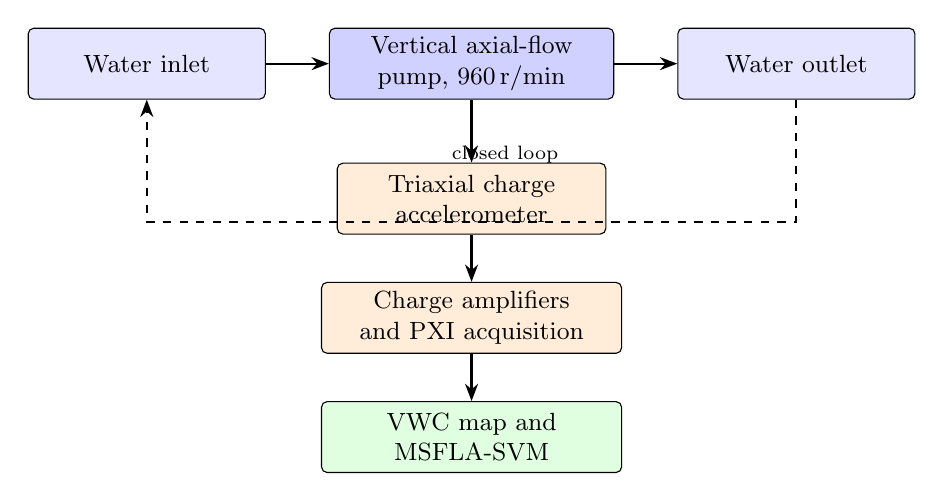
\begin{tikzpicture}[
  blk/.style={draw, rounded corners=2pt, align=center, font=\small, inner sep=3pt, minimum height=9mm},
  arr/.style={-{Stealth[length=2.2mm]}, thick}
]
  \node[blk, fill=blue!10, text width=28mm] (in) {Water inlet};
  \node[blk, fill=blue!18, text width=34mm, right=8mm of in] (pump) {Vertical axial-flow\\pump, \(960\,\mathrm{r/min}\)};
  \node[blk, fill=blue!10, text width=28mm, right=8mm of pump] (out) {Water outlet};
  \node[blk, fill=orange!15, text width=32mm, below=8mm of pump] (sen) {Triaxial charge\\accelerometer};
  \node[blk, fill=orange!15, text width=36mm, below=6mm of sen] (pxi) {Charge amplifiers\\and PXI acquisition};
  \node[blk, fill=green!12, text width=36mm, below=6mm of pxi] (pc) {VWC map and\\MSFLA-SVM};
  \draw[arr] (in) -- (pump);
  \draw[arr] (pump) -- (out);
  \draw[arr, dashed] (out.south) -- ++(0,-1.55) -| (in.south);
  \node[font=\scriptsize] at (4.55,-1.15) {closed loop};
  \draw[arr] (pump) -- (sen);
  \draw[arr] (sen) -- (pxi);
  \draw[arr] (pxi) -- (pc);
\end{tikzpicture}
\caption{Schematic of the diagnostic build. The dashed path is the closed water loop. The solid vertical path is the measurement and decision chain.}
\label{fig:rig}
\end{figure}

\subsection{The four operating states and how they are produced}

The experiment defines four mutually exclusive states.
The healthy state is the pump at the duty of Table~\ref{tab:rig} with no intentional defect.
The other three states are produced by a physical change, not by a numerical simulation.

Eccentric-axle fault is produced by moving a weight on the shaft so that the mass center leaves the geometric axis.
In the language of \eqref{eq:rotor} the change is an increase of the unbalance \(m e\).
The expected stationary signature is a rise of the force at \(f_{0}\) and, because severity integrates velocity rather than a single Fourier coefficient, a rise of VIB.
Both are observed: severity goes from \(1.051\) to \(3.737\,\mathrm{mm/s}\), and the tangential coefficient spectrum peaks at \(f_{0}\) with a larger amplitude than in the healthy state.
The source also notes energy at \(28\), \(34\), and \(38\,\mathrm{Hz}\) and attributes it to crosstalk from other devices in the laboratory.
Those tones are not members of \(\mathcal{F}\).
A feature map that sampled only \(\mathcal{F}\) is, by design, partly protected from them, and a feature map that used the whole spectrum as a long vector would have to learn to ignore them from forty-five training records.
This is one practical reason the \(22\)-vector is short.

Bearing-pedestal fault begins in the rolling-element bearing and is observed at the pedestal that supports it.
The source describes the usual bearing sequence: fatigue, wear, and adhesion, followed by a periodic jump of the pedestal, a change of the support stiffness, and an impact.
The expected spectral signature of a stiffness that is not constant inside one revolution includes a half-order line.
The published reading matches that expectation in the tangential direction, where the coefficient spectrum peaks at \(\tfrac12 f_{0}=8\,\mathrm{Hz}\).
Severity barely moves, from \(1.051\) to \(1.161\,\mathrm{mm/s}\).
The pedestal state is therefore a shape fault rather than an intensity fault, which is why it is included.
A rig that only seeded unbalance would let severity do the classification and would not test VWC.

Sealing-ring wear is a degradation of the ring that limits backflow from the discharge side and that keeps the impeller from rubbing the casing.
Wear opens a leakage path and risks impeller damage.
The expected signature is a hydraulic load at shaft order and at twice shaft order, together with a half-order component from the resulting asymmetry.
The published reading again matches: severity rises to \(1.70024\,\mathrm{mm/s}\), intermediate between the healthy and the eccentric states, and the spectrum emphasizes \(f_{0}\), \(\tfrac12 f_{0}\), and \(2f_{0}\).
The tangential direction carries the largest amplitudes, as it does in the other three states.

The four states are run as four separate conditions.
The published study does not include mixed faults, a slow ramp from healthy to faulty, or a speed sweep.
The classifier is therefore a four-way state identifier at one duty point.
Extending it to mixed faults would require a new sample and a decision about whether the label set stays a partition.

\subsection{The sensor and the three directions}

The transducer is a B\&K~4321 triaxial charge accelerometer.
Table~\ref{tab:sensor} lists the characteristics the source prints.
The charge sensitivity is \(9.8\,\mathrm{pC/g}\) within \(\pm 2\%\), which is approximately one picocoulomb per metre per second squared, because standard gravity is \(9.81\,\mathrm{m/s}^{2}\).
The stated frequency range, \(0.1\,\mathrm{Hz}\) to \(12\,\mathrm{kHz}\), covers the shaft family and the resonances that dominate acceleration.
The amplitude range is \(500\,g\).
The time-domain plots in the source have peaks of roughly \(7\) to \(9\,\mathrm{m/s}^{2}\), about one \(g\), so the records sit far below the range limit and clipping is not the explanation of any class error.

\begin{table}[H]
\centering
\caption{Published transducer and acquisition parameters.}
\label{tab:sensor}
\begin{tabular}{lll}
\toprule
Element & Parameter & Value \\
\midrule
B\&K 4321 & Type & Triaxial charge accelerometer \\
 & Charge sensitivity & \(9.8\pm 2\%\,\mathrm{pC/g}\) \\
 & Frequency range & \(0.1\) to \(12\,000\,\mathrm{Hz}\) \\
 & Measuring range & \(500\,g\) \\
\midrule
PXI acquisition card & Sampling frequency & \(100\,\mathrm{Hz}\) to \(100\,\mathrm{kHz}\), set to \(10\,\mathrm{kHz}\) \\
 & Input channels & \(8\) \\
 & Input range & \(\pm 100\,\mathrm{mV}\) to \(\pm 10\,\mathrm{V}\) \\
 & Stated precision & \(\pm 0.1\%\) of full-scale range, DC \\
\bottomrule
\end{tabular}
\end{table}

Charge leaves the sensor and enters a charge amplifier, whose voltage output is sampled by a PXI card with eight input channels, a selectable range from \(\pm 100\,\mathrm{mV}\) to \(\pm 10\,\mathrm{V}\), and a stated DC accuracy of \(\pm 0.1\%\) of full scale.
Three of the eight channels are required, one per axis.
The card can sample at up to \(100\,\mathrm{kHz}\); the experiment sets \(10\,\mathrm{kHz}\).
The Nyquist frequency is therefore \(5\,\mathrm{kHz}\).
The sensor itself responds up to \(12\,\mathrm{kHz}\), which is above Nyquist, so an anti-alias filter before the converter is part of a correct build.
The source table does not list that filter.
A repetition of the rig should place the filter cutoff below \(5\,\mathrm{kHz}\) with a stopband that covers the sensor's remaining bandwidth, and should record the cutoff next to the sampling rate.
Without it, energy between \(5\) and \(12\,\mathrm{kHz}\) folds into the analysis band and can move both the winning wavelet level and the high-order amplitudes.

The three axes are radial, tangential, and axial relative to the vertical rotor.
Figure~\ref{fig:axes} names them.
Unbalance forces lie in the plane perpendicular to the shaft, so they drive the radial and tangential channels.
A vertical hydraulic load drives the axial channel.
The published coefficient spectra say that the tangential channel has the largest amplitudes in every state.
Keeping all three is still necessary, because the axial channel is where the pedestal fault shows the high-order growth at \(5f_{0}\) and \(6f_{0}\), and the radial channel is where the published severity is defined.

\begin{figure}[H]
\centering
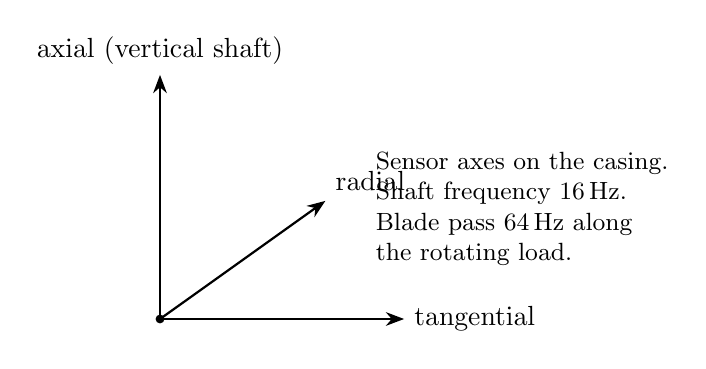
\begin{tikzpicture}[>=Stealth, thick]
  \draw[->] (0,0) -- (3.1,0) node[right] {tangential};
  \draw[->] (0,0) -- (0,3.1) node[above] {axial (vertical shaft)};
  \draw[->] (0,0) -- (2.1,1.5) node[above right] {radial};
  \fill (0,0) circle (1.6pt);
  \node[font=\small, align=left] at (4.6,1.4) {Sensor axes on the casing.\\Shaft frequency \(16\,\mathrm{Hz}\).\\Blade pass \(64\,\mathrm{Hz}\) along\\the rotating load.};
\end{tikzpicture}
\caption{The three measurement directions. The feature vector repeats the seven shaft-order amplitudes once in each direction and appends the radial severity.}
\label{fig:axes}
\end{figure}

\subsection{Sampling arithmetic}

Several numbers that the later estimate depends on are fixed by the clock and the record length, and they are worth writing once.
The sampling rate is \(f_{s}=10^{4}\,\mathrm{Hz}\).
The analysis length used to describe the records is \(N=8192\) samples, which is the right edge of the time-domain plots in the source.
The duration, the frequency resolution of a full-length Fourier transform, the number of shaft revolutions inside the record, and the Nyquist frequency are
\begin{align}
T_{\mathrm{rec}}&=\frac{N}{f_{s}}=\frac{8192}{10000}=0.8192\,\mathrm{s},&
\Delta f&=\frac{f_{s}}{N}=1.2207\,\mathrm{Hz},\\
N_{\mathrm{rev}}&=T_{\mathrm{rec}} f_{0}=13.107,&
f_{\mathrm{Nyq}}&=\frac{f_{s}}{2}=5\,\mathrm{kHz}.
\label{eq:arith}
\end{align}
Thirteen revolutions are enough for a stable estimate of a once-per-revolution line and are short enough that a pedestal impact does not have to be stationary over a long average.
The resolution \(1.2207\,\mathrm{Hz}\) puts \(3f_{0}=48\,\mathrm{Hz}\) and the supply line at \(50\,\mathrm{Hz}\) in different bins, with a gap of \(1.64\) bins.
An order sampler aimed at \(48\,\mathrm{Hz}\) with a half-order acceptance window of \(4\,\mathrm{Hz}\), as specified in Section~\ref{sec:vwc}, does not include \(50\,\mathrm{Hz}\).
That exclusion is deliberate.
It is also a limitation: a real supply harmonic that modulates a mechanical line inside the window will still be admitted.

At level \(j\) of a dyadic bank the coefficient rate is \(f_{s}/2^{j}\) and the length of the coefficient sequence is about \(N/2^{j}\).
For the level the source plots, \(j=5\), the coefficient rate is \(312.5\,\mathrm{Hz}\) and the coefficient record contains \(256\) samples.
A Fourier transform of those coefficients has a bin spacing of \(312.5/256=1.2207\,\mathrm{Hz}\), the same spacing as the full-length transform of the original record, and a coefficient-domain Nyquist of \(156.25\,\mathrm{Hz}\).
Every member of \(\mathcal{F}\), including \(6f_{0}=96\,\mathrm{Hz}\), lies inside that coefficient-domain Nyquist frequency.
The seven-order sampler is therefore well defined on \(d_{5}\) without a further resampling.
Had the winning level been \(d_{3}\), the coefficient Nyquist would have been \(625\,\mathrm{Hz}\) and the same orders would still lie inside it, with coarser relative localization.
Had the winning level been deeper than \(d_{7}\), the coefficient Nyquist would fall below \(96\,\mathrm{Hz}\) and \(6f_{0}\) would cease to be observable at that level.
The maximum-energy rule can in principle select such a level.
On the records the source plots, it selects \(d_{5}\), where all seven orders are observable.
An implementation should refuse an order that sits above the coefficient Nyquist of \(k^{\star}\) and should record the refusal, rather than report a folded frequency as if it were \(6f_{0}\).

\subsection{Sample size, split, and the unit of analysis}

The source collects \(60\) groups of data in each of the four states, \(240\) groups in all.
Each group is one \(22\)-vector.
Forty-five groups per state are the training sample and fifteen are the test sample, so the design matrices have shapes
\begin{equation}
\vect{X}_{\mathrm{train}}\in\R^{180\times 22},
\qquad
\vect{X}_{\mathrm{test}}\in\R^{60\times 22}.
\label{eq:shapes}
\end{equation}
The split is stratified by construction: each state contributes the same count to each matrix.
The source does not say whether the fifteen test groups were drawn at random, taken from the end of each run, or chosen by hand.
A repetition should draw them at random inside each state and should freeze the draw before any search over \((C, g)\).
Because the search described in Section~\ref{sec:svm} uses cross-validation inside the training matrix only, the sixty test rows are available for a single estimate.

Sixty test vectors is a small denominator.
One misclassified test vector moves a per-class rate by \(1/15\approx 6.67\) percentage points and moves the pooled rate by \(1/60\approx 1.67\) percentage points.
The difference between MSFLA-SVM and SFLA-SVM on the test set is one vector in the pooled count (\(56\) against \(55\)).
That difference is real as a count and it is small as evidence.
Section~\ref{sec:estimate} reports it as a count.

The source remarks that more records could not be collected under the conditions of the experiment, and that the SVM is used precisely because the sample is small.
The system build should be read with that constraint in view.
The acquisition is adequate for a four-class comparison at one duty.
It is not a durability test, and it is not a variable-speed campaign.

\subsection{The processing path}

Figure~\ref{fig:path} assembles the path from a stored record to a label.
The same path produces the training matrix and, with the normalization frozen, the test matrix.
Baselines branch after the normalization.
They do not receive a different feature.

The backpropagation baseline is the network of the kind Huang and Xie trained for bearing diagnosis~\cite{huang2009}, used here as the source uses it: a nonlinear classifier of the \(22\)-vector with no frog search.
The ACROA-SVM baseline is the radial SVM with parameters proposed by the artificial chemical reaction search of Alatas, in the bearing configuration of Ao, Cheng, Li, and Truong~\cite{ao2014,alatas2011}.
The SFLA-SVM baseline is the same radial SVM with the unmodified leap of Section~\ref{sec:svm}.
MSFLA-SVM is the modified leap.
All four see \(\tilde{\vect{x}}\) from \eqref{eq:norm}.
This common front end is what makes the table an estimate of classifiers rather than an estimate of features.
The source does not publish an ablation that removes severity, or the half-order, or one of the axes.
The present reading therefore cannot say which of the twenty-two coordinates carries the pedestal separation.
It can say that the full vector, shared by four classifiers, is sufficient for a pooled test accuracy above \(90\%\) for every SVM variant and not for the neural baseline.

\begin{figure}[H]
\centering
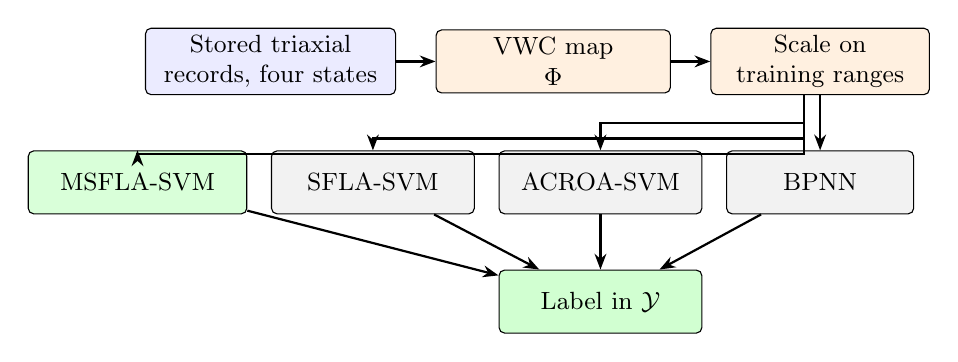
\begin{tikzpicture}[
  box/.style={draw, rounded corners=2pt, align=center, font=\small, inner sep=2.5pt, minimum height=8mm},
  arr/.style={-{Stealth[length=2mm]}, thick}
]
\node[box, fill=blue!8, text width=30mm] (rec) {Stored triaxial\\records, four states};
\node[box, fill=orange!12, text width=28mm, right=5mm of rec] (phi) {VWC map\\\(\Phi\)};
\node[box, fill=orange!12, text width=26mm, right=5mm of phi] (sc) {Scale on\\training ranges};
\node[box, fill=gray!10, text width=22mm, below=7mm of sc] (bp) {BPNN};
\node[box, fill=gray!10, text width=24mm, left=3mm of bp] (ac) {ACROA-SVM};
\node[box, fill=gray!10, text width=24mm, left=3mm of ac] (sf) {SFLA-SVM};
\node[box, fill=green!15, text width=26mm, left=3mm of sf] (ms) {MSFLA-SVM};
\node[box, fill=green!18, text width=24mm, below=7mm of ac] (lab) {Label in \(\mathcal{Y}\)};
\draw[arr] (rec) -- (phi);
\draw[arr] (phi) -- (sc);
\draw[arr] (sc) -- (bp);
\draw[arr] (sc.south) ++(-0.2,0) -- ++(0,-0.35) -| (ac.north);
\draw[arr] (sc.south) ++(-0.2,0) -- ++(0,-0.55) -| (sf.north);
\draw[arr] (sc.south) ++(-0.2,0) -- ++(0,-0.75) -| (ms.north);
\draw[arr] (ms) -- (lab);
\draw[arr] (sf) -- (lab);
\draw[arr] (ac) -- (lab);
\draw[arr] (bp) -- (lab);
\end{tikzpicture}
\caption{Processing path. The four classifiers are interchangeable blocks after a shared, train-scaled VWC vector.}
\label{fig:path}
\end{figure}

\subsection{What the build guarantees and what it leaves open}

The build guarantees a constant speed, a constant hydraulic duty, a triaxial casing measurement, a sampling rate that places the shaft family and the supply line on a resolvable grid, a record long enough for about thirteen revolutions, and a stratified sample of sixty vectors per state.
It leaves open the mother wavelet, the exact integrator inside the published severity, the anti-alias cutoff, the random seed of the split, and the population parameters of every evolutionary search.
Chapter~\ref{ch:methods} specified the wavelet, the normalization, the coding of the four classes, and the box of \((C, g)\) for this exposition, and it refused to invent the unpublished population parameters.
The estimate in the next section is attached to the source's run, under the source's unpublished choices, and the numerical values are taken from the source's tables.

\section{Estimation of diagnostic performance}
\label{sec:estimate}

\subsection{Signatures of the four states}
\label{sec:signatures}

The qualitative estimate comes before the percentages, because a classifier that scores well on a feature with no mechanical reading is a different claim from a classifier that scores well on VWC.
Table~\ref{tab:sign} compresses the source's reading of its time-domain records, its coefficient spectra, and its energy time-spectra.
Every state has its maximum wavelet energy at the \(d_{5}\) level in the radial plots the source prints.
The states differ in severity and in which member of \(\mathcal{F}\) dominates the tangential coefficient spectrum.

\begin{table}[H]
\centering
\caption{Published qualitative signatures of the four states, radial severity and tangential spectral emphasis.}
\label{tab:sign}
\small
\begin{tabular}{p{2.4cm}p{2.3cm}p{3.6cm}p{4.6cm}}
\toprule
State & Radial severity & Dominant tangential orders & Notes published with the records \\
\midrule
Normal & \(1.051\,\mathrm{mm/s}\) & \(f_{0}\), then \(2f_{0}\), \(3f_{0}\) & Supply line at \(50\,\mathrm{Hz}\); blade-pass energy at \(4f_{0}=64\,\mathrm{Hz}\). \\
EAF & \(3.737\,\mathrm{mm/s}\) & \(f_{0}\) & Crosstalk at \(28\), \(34\), and \(38\,\mathrm{Hz}\). Largest severity of the four states. \\
BPF & \(1.161\,\mathrm{mm/s}\) & \(\tfrac12 f_{0}\), with \(f_{0}\) and \(3f_{0}\) & High-order axial growth at \(5f_{0}\) and \(6f_{0}\), attributed to flow and to component natural frequencies. \\
SRWF & \(1.700\,\mathrm{mm/s}\) & \(f_{0}\), \(\tfrac12 f_{0}\), \(2f_{0}\) & Tangential energy is the largest; axial and radial intensities lie between EAF and BPF. \\
\bottomrule
\end{tabular}
\end{table}

A few published amplitudes make the tangential dominance quantitative.
Healthy tangential peak coefficient power is \(1.683\times 10^{-3}\) at \(f_{0}\).
Eccentric tangential peak power is \(3.322\times 10^{-3}\).
Pedestal tangential peak power is \(4.701\times 10^{-3}\) at \(\tfrac12 f_{0}\).
Healthy radial peak power is \(4.574\times 10^{-4}\), and eccentric radial peak power is \(2.492\times 10^{-3}\).
The pedestal tangential peak is about \(2.8\) times the healthy tangential peak, while the pedestal severity is only \(1.10\) times the healthy severity.
The spectral coordinate moves by a larger factor than the severity coordinate.
That comparison is the empirical reason the \(22\)-vector contains both, and the reason a severity threshold is not a substitute for the classifier.

The illustrative spectra in Figure~\ref{fig:spectra} were drawn to carry the same emphasis: healthy and eccentric energy at \(f_{0}\), pedestal and seal-wear energy with a stronger half-order.
They should be used as a picture of the emphasis and not as a source of amplitudes.
The amplitudes in the previous paragraph are the ones the source prints.

\subsection{Training estimate}

Training accuracy is the accuracy of each finished classifier on the \(180\) vectors it was trained on.
For the three SVM methods the finished classifier is the machine retrained on all \(180\) rows at the \((C, g)\) the search returned, so the training accuracy is an in-sample number and is expected to sit above the cross-validated fitness that guided the search.
Table~\ref{tab:train} gives the count of correct training vectors.
The percentages are those counts divided by \(45\), except where a printed percentage in the source decides an inconsistent count; the training table is internally consistent, and no such correction is required.
Each row average is the unweighted mean of the four method percentages, matching the source.
Each column average at the foot is the pooled accuracy, correct counts summed over states and divided by \(180\).

\begin{table}[H]
\centering
\caption{Training classification counts on \(45\) vectors per state. Pooled accuracy is correct-over-\(180\).}
\label{tab:train}
\begin{tabular}{lrrrrr}
\toprule
State & BPNN & ACROA-SVM & SFLA-SVM & MSFLA-SVM & Row mean \\
\midrule
Normal & 42/45 & 45/45 & 45/45 & 45/45 & 98.333\% \\
 & 93.333\% & 100\% & 100\% & 100\% & \\
EAF & 41/45 & 44/45 & 43/45 & 45/45 & 96.111\% \\
 & 91.111\% & 97.778\% & 95.556\% & 100\% & \\
BPF & 40/45 & 42/45 & 42/45 & 43/45 & 92.778\% \\
 & 88.889\% & 93.333\% & 93.333\% & 95.556\% & \\
SRWF & 42/45 & 44/45 & 44/45 & 44/45 & 96.667\% \\
 & 93.333\% & 97.778\% & 97.778\% & 97.778\% & \\
\midrule
Pooled & 165/180 & 175/180 & 174/180 & 177/180 & \\
 & 91.667\% & 97.222\% & 96.667\% & 98.333\% & \\
\bottomrule
\end{tabular}
\end{table}

The source prints the MSFLA pooled training accuracy as \(98.334\%\).
The exact ratio \(177/180\) is \(98.333\ldots\%\).
The difference is rounding.
This paper uses the ratio.

Figure~\ref{fig:train} shows the same rates.
Three facts are visible without the figure.
The healthy state is the easiest training class for every method, and every SVM variant classifies all \(45\) healthy training vectors correctly.
The pedestal state is the hardest training class for every method: \(40\), \(42\), \(42\), and \(43\) correct out of \(45\).
MSFLA-SVM is the unique method that classifies all \(45\) eccentric training vectors correctly, and it is tied or ahead on every state.
Its pooled gain over SFLA-SVM is three training vectors (\(177\) against \(174\)).
Its pooled gain over the neural baseline is twelve training vectors.

\begin{figure}[H]
\centering
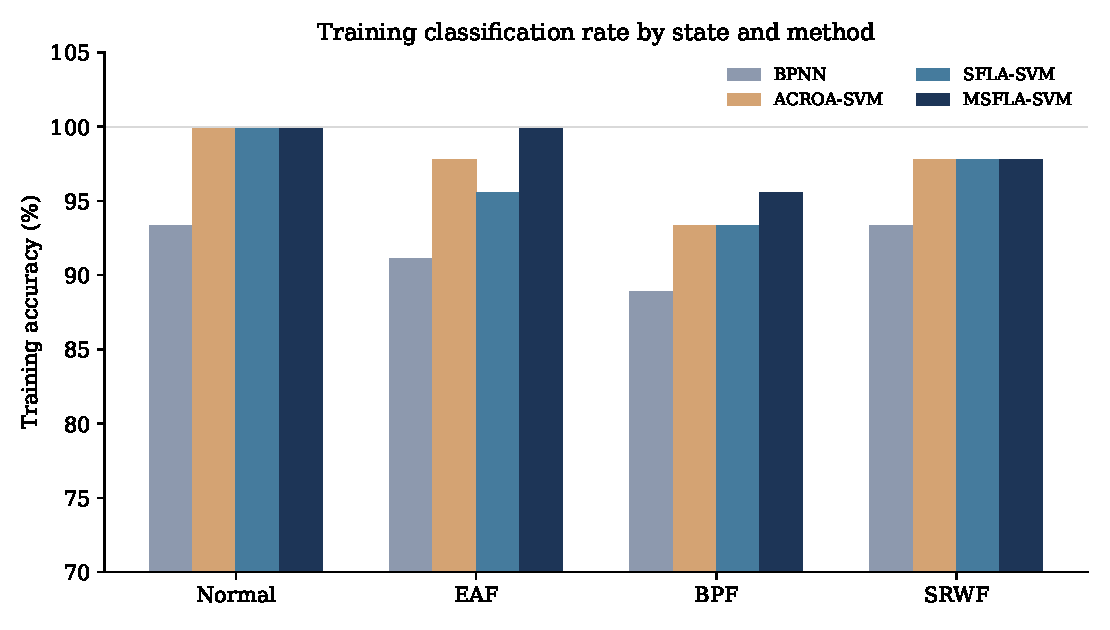
\includegraphics[width=0.92\textwidth]{train_accuracy.pdf}
\caption{Training accuracy by state and method, from Table~\ref{tab:train}.}
\label{fig:train}
\end{figure}

\subsection{Testing estimate}

Test accuracy is the quantity the search was not allowed to see.
Fifteen vectors per state, sixty in all, are labeled by the finished classifiers.
Table~\ref{tab:test} records the result.
For the backpropagation row of the sealing-ring state, the source prints a count of \(12/15\) beside a percentage of \(86.667\%\).
Those two entries disagree, because \(12/15=80\%\) and \(13/15=86.667\%\).
The four printed BPNN percentages \(86.667\), \(86.667\), \(80\), and \(86.667\) average to the printed pooled value \(85\%\), and the counts \(13\), \(13\), \(12\), and \(13\) sum to \(51\), with \(51/60=85\%\).
The count that agrees with the printed percentage and with the printed pooled accuracy is \(13/15\).
Table~\ref{tab:test} uses that count.
No other test cell requires a correction: ACROA, SFLA, and MSFLA are consistent with their pooled rates of \(91.667\%\), \(91.667\%\), and \(93.333\%\).

\begin{table}[H]
\centering
\caption{Test classification on \(15\) vectors per state. The BPNN entry for SRWF is \(13/15\), the count consistent with the printed percentage \(86.667\%\) and the printed pooled accuracy \(85\%\).}
\label{tab:test}
\begin{tabular}{lrrrrr}
\toprule
State & BPNN & ACROA-SVM & SFLA-SVM & MSFLA-SVM & Row mean \\
\midrule
Normal & 13/15 & 15/15 & 15/15 & 15/15 & 96.667\% \\
 & 86.667\% & 100\% & 100\% & 100\% & \\
EAF & 13/15 & 13/15 & 14/15 & 14/15 & 90.000\% \\
 & 86.667\% & 86.667\% & 93.333\% & 93.333\% & \\
BPF & 12/15 & 13/15 & 13/15 & 13/15 & 85.000\% \\
 & 80.000\% & 86.667\% & 86.667\% & 86.667\% & \\
SRWF & 13/15 & 14/15 & 13/15 & 14/15 & 90.000\% \\
 & 86.667\% & 93.333\% & 86.667\% & 93.333\% & \\
\midrule
Pooled & 51/60 & 55/60 & 55/60 & 56/60 & \\
 & 85.000\% & 91.667\% & 91.667\% & 93.333\% & \\
\bottomrule
\end{tabular}
\end{table}

\begin{figure}[H]
\centering
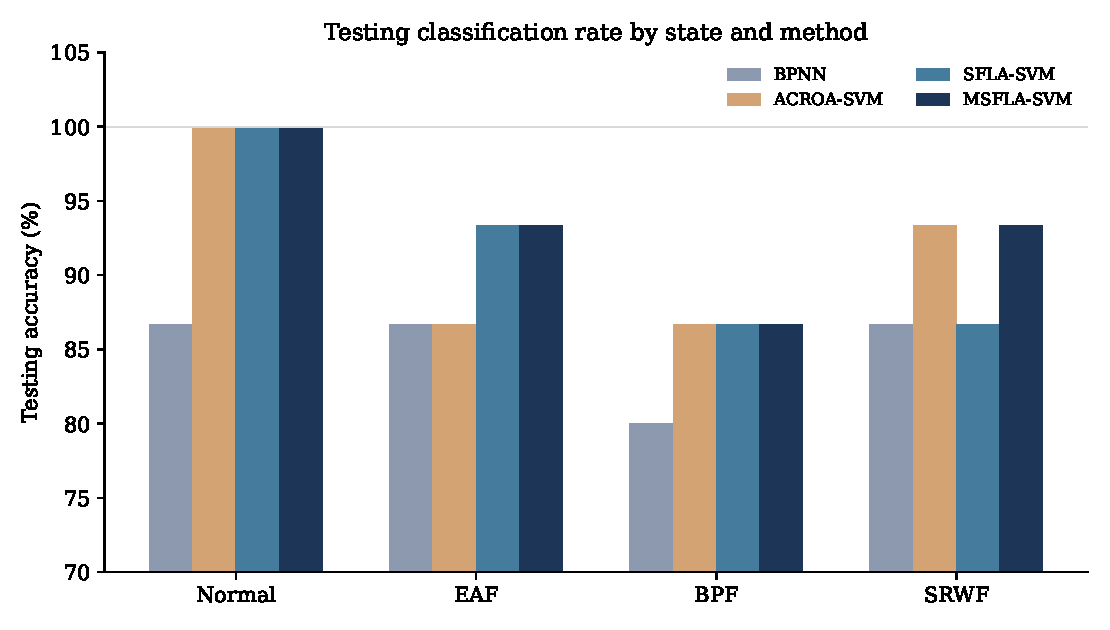
\includegraphics[width=0.92\textwidth]{test_accuracy.pdf}
\caption{Test accuracy by state and method, from Table~\ref{tab:test}. The pedestal state is the lowest bar in every group.}
\label{fig:test}
\end{figure}

\begin{figure}[H]
\centering
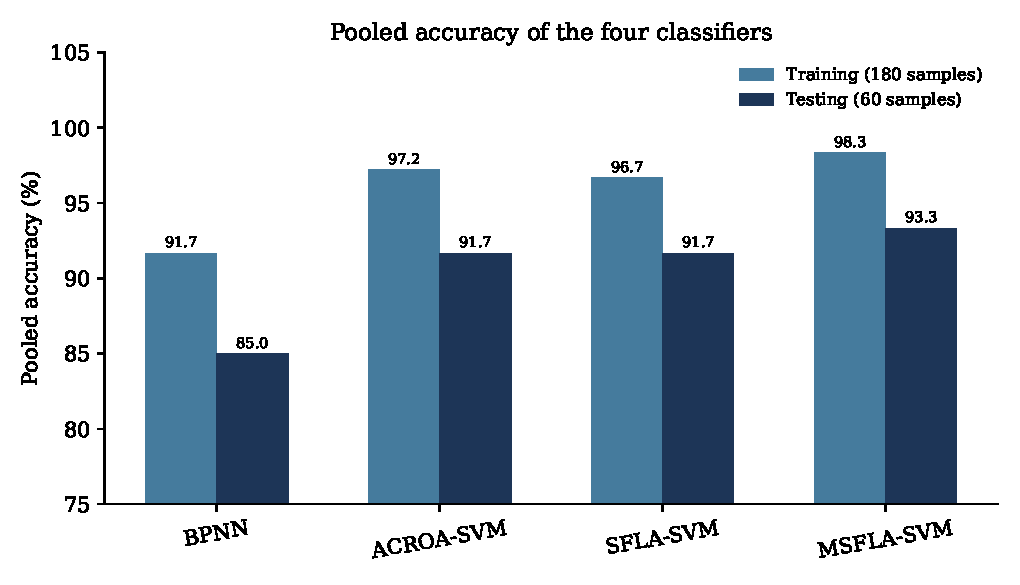
\includegraphics[width=0.82\textwidth]{pooled_accuracy.pdf}
\caption{Pooled training and test accuracy. The vertical gap inside each pair is the in-sample drop on \(60\) unseen vectors.}
\label{fig:pooled}
\end{figure}

The pooled test accuracies are \(85.0\%\) for the neural baseline, \(91.7\%\) for ACROA-SVM, \(91.7\%\) for SFLA-SVM, and \(93.3\%\) for MSFLA-SVM.
In counts, MSFLA-SVM labels \(56\) of the \(60\) test vectors correctly, the other two SVM searches label \(55\), and the neural baseline labels \(51\).
The modification of the leap is associated with one additional correct test vector relative to the unmodified leap and relative to the chemical-reaction search, and with five additional correct test vectors relative to the neural baseline.
Per state, MSFLA-SVM is never behind SFLA-SVM.
It ties SFLA-SVM on the healthy state (\(15/15\)), on the eccentric state (\(14/15\)), and on the pedestal state (\(13/15\)), and it labels one more sealing-ring vector correctly (\(14/15\) against \(13/15\)).
The entire pooled gain of the modification, on this test set, is that one sealing-ring vector.
Stating the result this way is more informative than stating only \(93.3\%\) against \(91.7\%\).

ACROA-SVM and SFLA-SVM land on the same pooled count by different per-class errors.
ACROA-SVM misses two eccentric vectors and one pedestal vector and one sealing-ring vector, in the sense that its correct counts are \(15\), \(13\), \(13\), and \(14\).
SFLA-SVM misses one eccentric vector, two pedestal vectors, and two sealing-ring vectors: correct counts \(15\), \(14\), \(13\), and \(13\).
The same number of errors is not the same error.
A maintenance decision that treats seal wear as more urgent than a mild eccentricity would prefer the ACROA pattern to the SFLA pattern even though the pooled rates match, and would prefer the MSFLA pattern to both because it keeps the ACROA seal-wear count and the SFLA eccentric count together.
The source does not publish the off-diagonal of the confusion matrix, so this paragraph accounts for misses per class and does not say which wrong label received them.

\subsection{Generalization drop}

The drop from pooled training accuracy to pooled test accuracy is a direct estimate of in-sample optimism:
\begin{equation}
\Delta = \mathrm{Acc}_{\mathrm{train}}-\mathrm{Acc}_{\mathrm{test}}.
\label{eq:drop}
\end{equation}
Table~\ref{tab:drop} evaluates \eqref{eq:drop} in percentage points and in counts.
The neural baseline drops \(6.67\) points, which is fourteen vectors of disagreement between the two rates' implied error counts (fifteen training errors out of \(180\), nine test errors out of \(60\)).
ACROA-SVM drops \(5.56\) points, SFLA-SVM drops \(5.00\) points, and MSFLA-SVM drops \(5.00\) points.
The modification does not enlarge the drop relative to the unmodified leap.
That fact matters because a search that found a higher training accuracy by memorizing the folds would usually pay for it on the test set.
MSFLA-SVM has both the highest training accuracy and the highest test accuracy, and its drop equals the drop of SFLA-SVM.
On a sample of this size the equality is one or two vectors, not a theorem.
It is still the right comparison to report, and it points in the direction the capacity argument of Chapter~\ref{ch:previous} predicts: the radial machines, all three of them, give up less accuracy when they leave the training sample than the neural baseline does.

\begin{table}[H]
\centering
\caption{Drop from pooled training accuracy to pooled test accuracy.}
\label{tab:drop}
\begin{tabular}{lrrr}
\toprule
Method & Training errors / 180 & Test errors / 60 & Drop (points) \\
\midrule
BPNN & 15 & 9 & 6.67 \\
ACROA-SVM & 5 & 5 & 5.56 \\
SFLA-SVM & 6 & 5 & 5.00 \\
MSFLA-SVM & 3 & 4 & 5.00 \\
\bottomrule
\end{tabular}
\end{table}

Per-class test means, averaged across the four methods as the source averages them, are \(96.667\%\) healthy, \(90\%\) eccentric, \(85\%\) pedestal, and \(90\%\) sealing-ring.
The healthy class is recognized by every SVM variant without a test error.
The pedestal class contributes two test errors to each SVM variant and three to the neural baseline.
The source's explanation is the one the signatures support.
The raw pedestal record is restricted by component resonance and by field interference, so the high-order coordinates that should describe the fault are also the coordinates the interference occupies.
VWC does not include a spatial filter or a coherence test against a second sensor that could reject a site tone.
The residual confusion is therefore a property of the measurement, and a better leap does not remove it.
MSFLA-SVM ties the other SVM methods at \(13/15\) on this class.
The open improvement the source itself names, better signal conditioning and less interference, sits in front of \(\Phi\), not inside the leap.

\subsection{How large the differences are}

A honest estimate states a difference in the unit the experiment controls, which is the labeled vector.
On the test set:
\begin{itemize}
\item MSFLA-SVM against BPNN: five vectors, \(56\) against \(51\), pooled rates \(93.333\%\) against \(85.000\%\).
\item MSFLA-SVM against ACROA-SVM: one vector, \(56\) against \(55\).
\item MSFLA-SVM against SFLA-SVM: one vector, \(56\) against \(55\), and that vector is a sealing-ring case.
\item ACROA-SVM against SFLA-SVM: zero vectors in the pooled count, with a different distribution across classes.
\end{itemize}
A five-vector gap against the neural baseline, on a sixty-vector test set, is large enough to be visible state by state: the neural baseline is behind on every state.
A one-vector gap between two global searches is the smallest nonzero gap the experiment can print.
It is consistent with the claim that the modified leap is not worse than the unmodified leap or the chemical-reaction search, and it is thin evidence for a claim that the modified leap is largely better.
The training table, where MSFLA-SVM leads by three vectors over SFLA-SVM and by two over ACROA-SVM, points the same way with a slightly larger count.
This paper reports both tables and does not promote the test gap of one vector into a percentage-point slogan detached from the denominator.

No confidence interval is published by the source, and none is fabricated here from an independence assumption the split may not obey.
If a reader assumes independent Bernoulli trials with success probability \(0.933\) and sixty trials, the standard deviation of the pooled accuracy is about \(\sqrt{0.933\cdot 0.067/60}\approx 0.032\), a little over three points, comparable to the gap between MSFLA-SVM and the neural baseline and larger than the gap between MSFLA-SVM and the other SVM searches.
The assumption is stronger than the evidence, because vectors from the same physical run are dependent.
The arithmetic is recorded only to show that the one-vector gap sits inside ordinary binomial variation and the five-vector gap sits at its edge.
A definitive ranking of the three searches would need a larger test set or a repeated split.

\subsection{What the estimate establishes}

The estimate establishes the following, and no more than the following.
\begin{enumerate}
\item The VWC vector, built from radial severity and from seven shaft-order coefficient amplitudes in three directions, separates the healthy pump from the three seeded faults well enough that a radial SVM labels at least \(55\) of \(60\) held-out vectors correctly.
\item The healthy state is linearly obvious in this vector for every SVM search: \(15\) of \(15\) test vectors, and \(45\) of \(45\) training vectors.
\item The eccentric state is the intensity fault.
Its severity is \(3.737\,\mathrm{mm/s}\) against \(1.051\,\mathrm{mm/s}\), and its test accuracy under MSFLA-SVM is \(14/15\).
\item The pedestal state is the shape fault and the hard fault.
Its severity is close to the healthy severity, its tangential energy moves to \(\tfrac12 f_{0}\), and every method, including the modified search, misses at least two of its fifteen test vectors.
\item On a shared VWC vector, the modified leap reaches a higher training count (\(177/180\)) and a higher test count (\(56/60\)) than the unmodified leap (\(174/180\) and \(55/60\)) and than the chemical-reaction search (\(175/180\) and \(55/60\)).
The test margin over each of those searches is one vector.
\item The backpropagation baseline, on the same vector, reaches \(165/180\) in training and \(51/60\) in testing.
The margin of MSFLA-SVM over this baseline is twelve training vectors and five test vectors, and the baseline's train-to-test drop is the largest of the four.
\end{enumerate}

\subsection{What the estimate does not establish}

The estimate does not establish a detection latency, because the records are labeled conditions rather than a timed evolution from healthy to faulty.
It does not establish performance at any speed other than \(960\,\mathrm{r/min}\), at any flow other than \(550\,\mathrm{m}^{3}/\mathrm{h}\), or under a mixture of two faults.
It does not establish which coordinate of the \(22\)-vector is necessary, because no ablation is published.
It does not establish the numerical pair \((C, g)\) that the leap returned, nor the population size, nor the number of shuffles.
It does not establish that db4 was the mother wavelet of the 2019 run; db4 is the wavelet of the illustrative energy figure and of the specification in Chapter~\ref{ch:methods}.
It does not establish a ranking of MSFLA against every published optimizer.
Particle swarm, genetic algorithm, and bee colony do not appear in the pump tables.
The related work reviewed in Chapter~\ref{ch:previous} shows that those searches are competitive on other machines.
A claim that the distance-weighted leap dominates them on this pump would be a new experiment.

The illustrative signals support none of the six positive statements above.
Those statements rest on the published severities, the published spectral reading, and the published counts.
The signals support only the narrower pedagogical claim that a record with the published severity and the published harmonic emphasis looks like Figure~\ref{fig:waves} and Figure~\ref{fig:spectra}, and that a db4 bank applied to such a record produces a nontrivial scale distribution, Figure~\ref{fig:energy}.

\subsection{Reading the result against the problem statement}

Section~\ref{sec:problem} asked for four things: a \(22\)-dimensional feature that carries intensity, scale, and shaft order; a leap that uses both leaders and that mutates locally; a build that makes the feature meaningful; and an estimate that respects the denominator of the test set.
The feature is specified in Section~\ref{sec:vwc} and is the common input of Table~\ref{tab:test}.
The leap is specified in Section~\ref{sec:svm} and is the unique difference between the SFLA column and the MSFLA column.
The build is specified in Section~\ref{sec:build}, and the arithmetic \eqref{eq:arith} shows that the clock matches the frequency family the feature samples.
The estimate is Table~\ref{tab:test} read in counts.
On those terms the pair of technologies does what the source claimed in direction and in magnitude: the modified search is the best of the four printed methods, the gain over the unmodified search is small, and the pedestal fault remains the open class.
The practical recommendation that follows is modest and precise.
Use the VWC vector rather than severity alone, because the pedestal fault is invisible to severity.
Use a radial SVM rather than the unconstrained neural baseline on a training set of \(180\) vectors, because the test drop is smaller and the test count is higher.
Use the modified leap in preference to the unmodified leap if the implementation cost is the same, and do not expect more than a vector or two on a test set of sixty.
Spend the next experimental effort on the interference in the pedestal records, which is where all four methods already agree that the present vector is weakest.

\subsection{Reproducibility notes}

A third party who rebuilds the system from this paper and from the source can match the following without access to the unpublished raw waveforms: the shaft frequency, the blade-pass frequency, the record duration, the Fourier resolution, the coefficient-domain Nyquist at level \(5\), the shapes of the two design matrices, every cell of the corrected test table, and every cell of the training table.
Matching the classifier byte for byte additionally requires the raw records, the mother wavelet, the integrator, the split, the search box actually used, and the population schedule.
The source states that the data are available from the corresponding authors on request.
Until those records are in hand, the illustrative figures of this paper should stay captioned as illustrations, and the tables of this chapter should stay captioned as a reading of the published counts.
That division is the reproducibility condition of the estimate.

\subsection{Error budget of the measurement chain}
\label{sec:budget}

The classification counts already include every error the chain actually made.
A separate budget is still useful, because it shows which contributions are large enough to move a feature and which are not.
Start from the sensor.
The B\&K~4321 charge sensitivity is stated as \(9.8\,\mathrm{pC/g}\) within \(\pm 2\%\).
A two-percent scale error multiplies every acceleration sample on that axis by a factor between \(0.98\) and \(1.02\).
Severity, being an RMS of a quantity linear in acceleration, inherits the same relative error:
\begin{equation}
\frac{\Delta\mathrm{VIB}}{\mathrm{VIB}}\approx 0.02.
\label{eq:senserr}
\end{equation}
On the healthy severity of \(1.051\,\mathrm{mm/s}\) this is about \(0.021\,\mathrm{mm/s}\).
On the eccentric severity of \(3.737\,\mathrm{mm/s}\) it is about \(0.075\,\mathrm{mm/s}\).
The gap between healthy and pedestal severities is \(1.161-1.051=0.110\,\mathrm{mm/s}\).
A two-percent calibration error is a fifth of that gap on the healthy reading and is smaller than the gap.
It does not by itself explain a confusion between those two states, and it is negligible beside the factor \(3.56\) that separates the eccentric state from the healthy state.
After the train-only normalization \eqref{eq:norm}, a pure scale error that is constant for the whole campaign is absorbed into \(u^{(j)}\) and \(v^{(j)}\) of the severity coordinate, provided the same sensor and the same gain are used for every record.
A scale error that changed between the training days and the test days would not be absorbed.
The source does not report a recalibration, and the budget assumes the gain was held fixed.

The acquisition card states a DC accuracy of \(\pm 0.1\%\) of full-scale range.
On the \(\pm 10\,\mathrm{V}\) range this is \(10\,\mathrm{mV}\).
On the \(\pm 100\,\mathrm{mV}\) range it is \(0.1\,\mathrm{mV}\).
Which range was selected is not printed.
The time-domain plots show accelerations of roughly \(7\) to \(9\,\mathrm{m/s}^{2}\), about one \(g\).
At \(9.8\,\mathrm{pC/g}\) that motion produces about \(10\,\mathrm{pC}\) at the peaks.
The voltage that results is the charge divided by the amplifier's feedback capacitance, a setting the source also does not print.
The relevant statement the budget can still make is comparative.
A full-scale error of \(0.1\%\) is twenty times smaller than the sensor's \(2\%\) sensitivity tolerance, so on any range that actually uses a reasonable fraction of its bits the card is not the leading scale error.
Quantization at, for example, a \(16\)-bit converter on a range matched to a few \(g\) sits well below both.
The chain is sensor-limited for amplitude, and it is clock-limited for frequency.

Clock error moves the orders in Table~\ref{tab:bins}.
A sampling-rate error of \(\varepsilon\) moves every apparent frequency by the same relative amount.
The widest order, \(6f_{0}=96\,\mathrm{Hz}\), moves by \(96\varepsilon\).
The half-order acceptance window specified for this exposition is \(4\,\mathrm{Hz}\).
Keeping the true \(6f_{0}\) inside that window requires
\begin{equation}
96\,\abs{\varepsilon}<4
\qquad\Rightarrow\qquad
\abs{\varepsilon}<0.042,
\label{eq:clock}
\end{equation}
a four-percent clock, which any PXI timebase meets by a wide margin.
The binding frequency constraint is not the clock.
It is the mechanical speed.
A one-percent speed drift, already discussed as an envelope of the method, moves \(6f_{0}\) by about \(1\,\mathrm{Hz}\), still inside the window, and moves the supply-to-\(3f_{0}\) gap from \(2.00\,\mathrm{Hz}\) to either \(1.52\,\mathrm{Hz}\) or \(2.48\,\mathrm{Hz}\) according to the sign.
The \(1.22\,\mathrm{Hz}\) bin can still hold them apart.
A speed that was only nominally \(960\,\mathrm{r/min}\), and that wandered by several percent inside a record, would broaden every order and would raise the pedestal and seal-wear confusion first, because those states are identified by which order is largest rather than by a large severity.
The source states a single speed.
The budget treats residual speed wander as an unquantified contribution inside the pedestal errors, not as a number the tables support.

Aliasing is the contribution the budget cannot bound from the printed table.
The sensor responds to \(12\,\mathrm{kHz}\) and the converter samples at \(10\,\mathrm{kHz}\), so energy between \(5\) and \(12\,\mathrm{kHz}\) folds into \(0\) to \(5\,\mathrm{kHz}\) unless an analog filter stops it.
Folded energy lands preferentially in the fine wavelet levels, and it can change which level wins \(k^{\star}\).
If the winning level moves, the coefficient rate changes and the amplitudes \eqref{eq:samples} are read on a different series.
The source plots show \(d_{5}\) winning for the displayed records, which is evidence that, on those records, the mid band carried the energy, and it is not evidence that an anti-alias filter was present.
A repetition of the build should state the filter cutoff next to the \(10\,\mathrm{kHz}\) clock.
Until that cutoff is known, high-frequency folding remains an open term in the budget and a candidate contributor to the two pedestal test errors that every SVM method still makes.

Interference tones that the order sampler does not aim at --- the reported crosstalk at \(28\), \(34\), and \(38\,\mathrm{Hz}\) under the eccentric fault, and the supply line at \(50\,\mathrm{Hz}\) --- are rejected by the sampler's narrow windows and are not rejected by the wavelet energy that chooses the level.
They can change \(k^{\star}\) without entering \(\vect{x}\) as their own coordinates.
That indirect path is the reason a clean mechanical spectrum and a clean scale choice are both part of signal conditioning, which is the improvement the source itself defers to future work.
The budget's conclusion is short.
Calibration and quantization are too small to explain the published confusions.
Speed error at the one-percent level is tolerable for the order windows.
Unfiltered high-frequency energy and in-band interference are large enough, in mechanism, to move the pedestal features, and they are exactly the mechanisms named in the source discussion of that class.

\subsection{An operating procedure for one labeled record}
\label{sec:procedure}

The build is reproducible as a sequence even where some numerical settings remain those of the original run.
One labeled record, from the command to start the pump through the row that enters \(\vect{X}\), is the following procedure.
It is the system of Section~\ref{sec:build} written as steps an operator can tick, not as a new experiment.
\begin{enumerate}
\item Set the loop to the duty in Table~\ref{tab:rig}: \(960\,\mathrm{r/min}\), \(550\,\mathrm{m}^{3}/\mathrm{h}\), \(3\,\mathrm{m}\) head, four-blade impeller, closed circuit.
Confirm \(f_{0}=16\,\mathrm{Hz}\) from a tachometer or from the once-per-revolution line before any fault label is trusted.
\item Install the fault for this record, or install none.
Eccentric axle: displace the balance weight and record the mass and the radius, even though the classifier never sees those two numbers, because a later reader of the severity \(3.737\,\mathrm{mm/s}\) will want them.
Pedestal: seed the bearing defect the campaign has defined and confirm that the pedestal is the vibrating part under the sensor.
Seal wear: use the worn ring the campaign has defined and confirm that the impeller is not rubbing.
Do not combine two of these in one record.
The label set is a partition.
\item Mount the triaxial charge accelerometer on the casing.
Note the direction that will be called radial, because that direction supplies the single severity coordinate.
Check that the charge cables and the amplifier gains are the same ones used for the records already in the training matrix.
\item Set the converter to \(10\,\mathrm{kHz}\), confirm the anti-alias cutoff is below \(5\,\mathrm{kHz}\), and arm a capture of at least \(8192\) samples on all three axes after the pump has been at speed long enough for the flow to be steady.
Store the three series and the tachometer reading with the state label.
\item Compute radial severity by the campaign's stated integrator and by \eqref{eq:vibdisc}.
Run the eight-level db4 bank on each axis, select \(k^{\star}\) by \eqref{eq:kstar} with the finer level winning a tie, and sample the seven orders of \eqref{eq:ordersexact} from the coefficient power spectrum \eqref{eq:cps} through the frequency map \eqref{eq:fmap}.
Refuse any order above the coefficient Nyquist of the winning level.
\item Assemble \eqref{eq:x22}.
If the row is a training row, update nothing about scaling until the full training matrix exists, then fit \eqref{eq:norm}.
If the row is a test row, apply the training ranges already stored.
Do not refit them.
\item When \(180\) training rows are in hand, run the modified leap inside the box \eqref{eq:box} with fitness \eqref{eq:fitness}, retrain the six binary machines on all \(180\) rows at the returned pair, and only then label the \(60\) test rows by vote.
Log the six items of Section~\ref{sec:cost}.
\end{enumerate}
Steps 1--4 are the rig.
Steps 5 and 6 are VWC.
Step 7 is MSFLA-SVM.
A baseline replaces step 7 and does not replace steps 1--6.
That separation is what makes Table~\ref{tab:test} a comparison of classifiers on one feature.

The procedure also says what the operator does not do.
The operator does not choose \(C\) and \(g\) by hand after looking at the test labels.
The operator does not drop the pedestal records because they are harder.
The operator does not lengthen the test set by moving training rows across the split after the search has run.
Each of those moves would raise a number in Table~\ref{tab:test} and would destroy the estimate.
The published counts are informative because, as far as the source text shows, none of those moves was made.

\subsection{The estimate in the unit the experiment controls}
\label{sec:unit}

Table~\ref{tab:errors} restates the published result as error counts, which is the unit in which a one-vector gap is not asked to look like a percentage-point discovery.
Training errors are out of \(180\).
Test errors are out of \(60\).
The per-class test errors follow by subtracting the correct counts of Table~\ref{tab:test} from \(15\).

\begin{table}[H]
\centering
\caption{Error counts. Training errors are out of \(180\) pooled vectors. Test errors are out of \(60\) pooled vectors, and the four class columns are out of \(15\).}
\label{tab:errors}
\begin{tabular}{lrrrrrr}
\toprule
Method & Train & Test & Normal & EAF & BPF & SRWF \\
\midrule
BPNN & 15 & 9 & 2 & 2 & 3 & 2 \\
ACROA-SVM & 5 & 5 & 0 & 2 & 2 & 1 \\
SFLA-SVM & 6 & 5 & 0 & 1 & 2 & 2 \\
MSFLA-SVM & 3 & 4 & 0 & 1 & 2 & 1 \\
\bottomrule
\end{tabular}
\end{table}

Read across the test columns, the modified search matches the better of the other two searches in every state: it matches SFLA-SVM on the eccentric axle (one error), matches both SVM searches on the pedestal (two errors), matches ACROA-SVM on seal wear (one error), and matches every SVM search on the healthy state (no error).
It does not create a new kind of success on the pedestal.
It collects, in one rule, the per-class results that the other searches hold only separately.
That is a fair description of a one-vector pooled gain, and it is the description this estimate keeps.

Read down the pedestal column, no method is in single digits of a different kind: the best pedestal result on the test set is two errors out of fifteen, which is \(13/15\).
The training pedestal column of Table~\ref{tab:train} is consistent with the same ranking.
MSFLA-SVM misses two of forty-five pedestal training vectors, and every other method misses more.
The feature, not the leap, is saturated on this class.
Further optimization of \((C, g)\) can rearrange one error among the easier classes, which is what the sealing-ring column shows, and it has not been observed to buy a pedestal test vector.

The practical statement that closes the estimate is therefore a statement about effort.
On this rig, with this sample, the VWC vector plus a radial SVM already carries the diagnosis from the neural baseline's nine test errors to five.
The modified leap carries it from five to four, by avoiding one seal-wear error that the unmodified leap makes and one eccentric error that the chemical-reaction search makes.
The two pedestal errors that remain are the next experiment: a second sensor, a stated anti-alias filter, or a conditioning step aimed at the site tones, scored on a new split.
They are not a reason to discard the twenty-two coordinates or the leap that reads them.
They are the part of the problem the published counts show is still open.


\begin{thebibliography}{99}

\bibitem{you2019}
L.~You, W.~Fan, Z.~Li, Y.~Liang, M.~Fang, and J.~Wang,
``A fault diagnosis model for rotating machinery using VWC and MSFLA-SVM based on vibration signal analysis,''
\textit{Shock and Vibration}, vol.~2019, Article ID 1908485, 2019.

\bibitem{sohre1968}
J.~S.~Sohre,
``Operating problems with high-speed turbomachinery---causes and correction,''
in \textit{Proceedings of the 23rd Annual Petroleum Mechanical Engineering Conference}, Dallas, TX, USA, 1968.

\bibitem{beard1971}
R.~V.~Beard,
\textit{Failure Accommodation in Linear Systems through Self-Reorganization},
Ph.D.\ thesis, Massachusetts Institute of Technology, Cambridge, MA, USA, 1971.

\bibitem{willsky1976}
A.~S.~Willsky,
``A survey of design methods for failure detection in dynamic systems,''
\textit{Automatica}, vol.~12, no.~6, pp.~601--611, 1976.

\bibitem{mcfadden1984}
P.~D.~McFadden and J.~D.~Smith,
``Model for the vibration produced by a single point defect in a rolling element bearing,''
\textit{Journal of Sound and Vibration}, vol.~96, no.~1, pp.~69--82, 1984.

\bibitem{grossmann1984}
A.~Grossmann and J.~Morlet,
``Decomposition of Hardy functions into square integrable wavelets of constant shape,''
\textit{SIAM Journal on Mathematical Analysis}, vol.~15, no.~4, pp.~723--736, 1984.

\bibitem{daubechies1988}
I.~Daubechies,
``Orthonormal bases of compactly supported wavelets,''
\textit{Communications on Pure and Applied Mathematics}, vol.~41, no.~7, pp.~909--996, 1988.

\bibitem{mallat1989}
S.~G.~Mallat,
``A theory for multiresolution signal decomposition: the wavelet representation,''
\textit{IEEE Transactions on Pattern Analysis and Machine Intelligence}, vol.~11, no.~7, pp.~674--693, 1989.

\bibitem{cooley1965}
J.~W.~Cooley and J.~W.~Tukey,
``An algorithm for the machine calculation of complex Fourier series,''
\textit{Mathematics of Computation}, vol.~19, no.~90, pp.~297--301, 1965.

\bibitem{welch1967}
P.~D.~Welch,
``The use of fast Fourier transform for the estimation of power spectra: a method based on time averaging over short, modified periodograms,''
\textit{IEEE Transactions on Audio and Electroacoustics}, vol.~15, no.~2, pp.~70--73, 1967.

\bibitem{mercer1909}
J.~Mercer,
``Functions of positive and negative type and their connection with the theory of integral equations,''
\textit{Philosophical Transactions of the Royal Society A}, vol.~209, pp.~415--446, 1909.

\bibitem{cover1965}
T.~M.~Cover,
``Geometrical and statistical properties of systems of linear inequalities with applications in pattern recognition,''
\textit{IEEE Transactions on Electronic Computers}, vol.~EC-14, no.~3, pp.~326--334, 1965.

\bibitem{frank1990}
P.~M.~Frank,
``Fault diagnosis in dynamic systems using analytical and knowledge-based redundancy---a survey and some new results,''
\textit{Automatica}, vol.~26, no.~3, pp.~459--474, 1990.

\bibitem{boser1992}
B.~E.~Boser, I.~M.~Guyon, and V.~N.~Vapnik,
``A training algorithm for optimal margin classifiers,''
in \textit{Proceedings of the Fifth Annual Workshop on Computational Learning Theory}, pp.~144--152, 1992.

\bibitem{vapnik1995}
V.~N.~Vapnik,
\textit{The Nature of Statistical Learning Theory}.
New York: Springer, 1995.

\bibitem{cortes1995}
C.~Cortes and V.~Vapnik,
``Support-vector networks,''
\textit{Machine Learning}, vol.~20, no.~3, pp.~273--297, 1995.

\bibitem{holland1975}
J.~H.~Holland,
\textit{Adaptation in Natural and Artificial Systems}.
Ann Arbor, MI: University of Michigan Press, 1975.

\bibitem{kennedy1995}
J.~Kennedy and R.~Eberhart,
``Particle swarm optimization,''
in \textit{Proceedings of the IEEE International Conference on Neural Networks}, pp.~1942--1948, 1995.

\bibitem{platt1999}
J.~Platt,
``Fast training of support vector machines using sequential minimal optimization,''
in B.~Sch\"olkopf, C.~J.~C.~Burges, and A.~J.~Smola, Eds., \textit{Advances in Kernel Methods---Support Vector Learning}.
Cambridge, MA: MIT Press, 1999.

\bibitem{suykens1999}
J.~A.~K.~Suykens and J.~Vandewalle,
``Least squares support vector machine classifiers,''
\textit{Neural Processing Letters}, vol.~9, no.~3, pp.~293--300, 1999.

\bibitem{tandon1999}
N.~Tandon and A.~Choudhury,
``A review of vibration and acoustic measurement methods for the detection of defects in rolling element bearings,''
\textit{Tribology International}, vol.~32, no.~8, pp.~469--480, 1999.

\bibitem{edwards2000}
C.~Edwards, S.~K.~Spurgeon, and R.~J.~Patton,
``Sliding mode observers for fault detection and isolation,''
\textit{Automatica}, vol.~36, no.~4, pp.~541--553, 2000.

\bibitem{li2000}
B.~Li, M.-Y.~Chow, Y.~Tipsuwan, and J.~C.~Hung,
``Neural-network-based motor rolling bearing fault diagnosis,''
\textit{IEEE Transactions on Industrial Electronics}, vol.~47, no.~5, pp.~1060--1069, 2000.

\bibitem{persis2001}
C.~De~Persis and A.~Isidori,
``A differential-geometric approach to nonlinear fault detection and isolation,''
\textit{IEEE Transactions on Automatic Control}, vol.~46, no.~6, pp.~853--865, 2001.

\bibitem{huang1998}
N.~E.~Huang, Z.~Shen, S.~R.~Long, M.~C.~Wu, H.~H.~Shih, Q.~Zheng, N.-C.~Yen, C.~C.~Tung, and H.~H.~Liu,
``The empirical mode decomposition and the Hilbert spectrum for nonlinear and non-stationary time series analysis,''
\textit{Proceedings of the Royal Society A}, vol.~454, pp.~903--995, 1998.

\bibitem{jack2002}
L.~B.~Jack and A.~K.~Nandi,
``Fault detection using support vector machines and artificial neural networks, augmented by genetic algorithms,''
\textit{Mechanical Systems and Signal Processing}, vol.~16, nos.~2--3, pp.~373--390, 2002.

\bibitem{samanta2003}
B.~Samanta and K.~R.~Al-Balushi,
``Artificial neural network based fault diagnostics of rolling element bearings using time-domain features,''
\textit{Mechanical Systems and Signal Processing}, vol.~17, no.~2, pp.~317--328, 2003.

\bibitem{venkat2003}
V.~Venkatasubramanian, R.~Rengaswamy, K.~Yin, and S.~N.~Kavuri,
``A review of process fault detection and diagnosis. Part~I: Quantitative model-based methods,''
\textit{Computers and Chemical Engineering}, vol.~27, no.~3, pp.~293--311, 2003.

\bibitem{eusuff2003}
M.~M.~Eusuff and K.~E.~Lansey,
``Optimization of water distribution network design using the shuffled frog leaping algorithm,''
\textit{Journal of Water Resources Planning and Management}, vol.~129, no.~3, pp.~210--225, 2003.

\bibitem{peng2004}
Z.~K.~Peng and F.~L.~Chu,
``Application of the wavelet transform in machine condition monitoring and fault diagnostics: a review,''
\textit{Mechanical Systems and Signal Processing}, vol.~18, no.~2, pp.~199--221, 2004.

\bibitem{samanta2004}
B.~Samanta,
``Gear fault detection using artificial neural networks and support vector machines with genetic algorithms,''
\textit{Mechanical Systems and Signal Processing}, vol.~18, no.~3, pp.~625--644, 2004.

\bibitem{lou2004}
X.~Lou and K.~A.~Loparo,
``Bearing fault diagnosis based on wavelet transform and fuzzy inference,''
\textit{Mechanical Systems and Signal Processing}, vol.~18, no.~5, pp.~1077--1095, 2004.

\bibitem{isermann2005}
R.~Isermann,
``Model-based fault-detection and diagnosis---status and applications,''
\textit{Annual Reviews in Control}, vol.~29, no.~1, pp.~71--85, 2005.

\bibitem{smith2005}
J.~S.~Smith,
``The local mean decomposition and its application to EEG perception data,''
\textit{Journal of the Royal Society Interface}, vol.~2, no.~5, pp.~443--454, 2005.

\bibitem{antoni2006}
J.~Antoni,
``The spectral kurtosis: a useful tool for characterising non-stationary signals,''
\textit{Mechanical Systems and Signal Processing}, vol.~20, no.~2, pp.~282--307, 2006.

\bibitem{jardine2006}
A.~K.~S.~Jardine, D.~Lin, and D.~Banjevic,
``A review on machinery diagnostics and prognostics implementing condition-based maintenance,''
\textit{Mechanical Systems and Signal Processing}, vol.~20, no.~7, pp.~1483--1510, 2006.

\bibitem{eusuff2006}
M.~Eusuff, K.~Lansey, and F.~Pasha,
``Shuffled frog-leaping algorithm: a memetic meta-heuristic for discrete optimization,''
\textit{Engineering Optimization}, vol.~38, no.~2, pp.~129--154, 2006.

\bibitem{hu2007}
Q.~Hu, Z.~He, Z.~Zhang, and Y.~Zi,
``Fault diagnosis of rotating machinery based on improved wavelet package transform and SVMs ensemble,''
\textit{Mechanical Systems and Signal Processing}, vol.~21, no.~2, pp.~688--705, 2007.

\bibitem{widodo2007}
A.~Widodo and B.-S.~Yang,
``Support vector machine in machine condition monitoring and fault diagnosis,''
\textit{Mechanical Systems and Signal Processing}, vol.~21, no.~6, pp.~2560--2574, 2007.

\bibitem{karaboga2007}
D.~Karaboga and B.~Basturk,
``A powerful and efficient algorithm for numerical function optimization: artificial bee colony (ABC) algorithm,''
\textit{Journal of Global Optimization}, vol.~39, no.~3, pp.~459--471, 2007.

\bibitem{lei2008}
Y.~Lei, Z.~He, and Y.~Zi,
``A new approach to intelligent fault diagnosis of rotating machinery,''
\textit{Expert Systems with Applications}, vol.~35, no.~4, pp.~1593--1600, 2008.

\bibitem{wu2009}
Z.~Wu and N.~E.~Huang,
``Ensemble empirical mode decomposition: a noise-assisted data analysis method,''
\textit{Advances in Adaptive Data Analysis}, vol.~1, no.~1, pp.~1--41, 2009.

\bibitem{huang2009}
Z.~G.~Huang and Y.~Xie,
``Fault diagnosis method of rolling bearing based on BP neural network,''
in \textit{Proceedings of the International Conference on Measuring Technology and Mechatronics Automation}, pp.~647--649, 2009.

\bibitem{saravanan2010}
N.~Saravanan and K.~I.~Ramachandran,
``Incipient gear box fault diagnosis using discrete wavelet transform (DWT) for feature extraction and classification using artificial neural network (ANN),''
\textit{Expert Systems with Applications}, vol.~37, no.~6, pp.~4168--4181, 2010.

\bibitem{kankar2011}
P.~K.~Kankar, S.~C.~Sharma, and S.~P.~Harsha,
``Fault diagnosis of ball bearings using machine learning methods,''
\textit{Expert Systems with Applications}, vol.~38, no.~3, pp.~1876--1886, 2011.

\bibitem{randall2011}
R.~B.~Randall and J.~Antoni,
``Rolling element bearing diagnostics---a tutorial,''
\textit{Mechanical Systems and Signal Processing}, vol.~25, no.~2, pp.~485--520, 2011.

\bibitem{huang2011}
J.~Huang, X.~Hu, and F.~Yang,
``Support vector machine with genetic algorithm for machinery fault diagnosis of high voltage circuit breaker,''
\textit{Measurement}, vol.~44, no.~6, pp.~1018--1027, 2011.

\bibitem{chang2011}
C.-C.~Chang and C.-J.~Lin,
``LIBSVM: A library for support vector machines,''
\textit{ACM Transactions on Intelligent Systems and Technology}, vol.~2, no.~3, Article~27, 2011.

\bibitem{alatas2011}
B.~Alatas,
``ACROA: Artificial chemical reaction optimization algorithm for global optimization,''
\textit{Expert Systems with Applications}, vol.~38, no.~10, pp.~13170--13180, 2011.

\bibitem{gao2011}
R.~X.~Gao and R.~Yan,
\textit{Wavelets: Theory and Applications for Manufacturing}.
New York: Springer, 2011.

\bibitem{scholkopf2002}
B.~Sch\"olkopf and A.~J.~Smola,
\textit{Learning with Kernels}.
Cambridge, MA: MIT Press, 2002.

\bibitem{hsu2003}
C.-W.~Hsu, C.-C.~Chang, and C.-J.~Lin,
``A practical guide to support vector classification,''
Technical report, National Taiwan University, Taipei, 2003.

\bibitem{bin2012}
G.~F.~Bin, J.~J.~Gao, X.~J.~Li, and B.~S.~Dhillon,
``Early fault diagnosis of rotating machinery based on wavelet packets--empirical mode decomposition feature extraction and neural network,''
\textit{Mechanical Systems and Signal Processing}, vol.~27, pp.~696--711, 2012.

\bibitem{lei2013}
Y.~Lei, J.~Lin, Z.~He, and M.~J.~Zuo,
``A review on empirical mode decomposition in fault diagnosis of rotating machinery,''
\textit{Mechanical Systems and Signal Processing}, vol.~35, nos.~1--2, pp.~108--126, 2013.

\bibitem{dong2013}
S.~Dong and T.~Luo,
``Bearing degradation process prediction based on the PCA and optimized LS-SVM model,''
\textit{Measurement}, vol.~46, no.~9, pp.~3143--3152, 2013.

\bibitem{seshadrinath2014}
J.~Seshadrinath, B.~Singh, and B.~K.~Panigrahi,
``Investigation of vibration signatures for multiple fault diagnosis in variable frequency drives using complex wavelets,''
\textit{IEEE Transactions on Power Electronics}, vol.~29, no.~2, pp.~936--945, 2014.

\bibitem{dybala2014}
J.~Dyba{\l}a and R.~Zimroz,
``Rolling bearing diagnosing method based on empirical mode decomposition of machine vibration signal,''
\textit{Applied Acoustics}, vol.~77, pp.~195--203, 2014.

\bibitem{bordoloi2014}
D.~J.~Bordoloi and R.~Tiwari,
``Optimum multi-fault classification of gears with integration of evolutionary and SVM algorithms,''
\textit{Mechanism and Machine Theory}, vol.~73, pp.~49--60, 2014.

\bibitem{dragomiretskiy2014}
K.~Dragomiretskiy and D.~Zosso,
``Variational mode decomposition,''
\textit{IEEE Transactions on Signal Processing}, vol.~62, no.~3, pp.~531--544, 2014.

\bibitem{cai2014}
B.~Cai, Y.~Liu, Q.~Fan, Y.~Zhang, Z.~Liu, S.~Yu, and R.~Ji,
``Multi-source information fusion based fault diagnosis of ground-source heat pump using Bayesian network,''
\textit{Applied Energy}, vol.~114, pp.~1--9, 2014.

\bibitem{ao2014}
H.~L.~Ao, J.~S.~Cheng, K.~L.~Li, and T.~K.~Truong,
``A roller bearing fault diagnosis method based on LCD energy entropy and ACROA-SVM,''
\textit{Shock and Vibration}, vol.~2014, Article ID 825825, 2014.

\bibitem{tian2015}
Y.~Tian, J.~Ma, C.~Lu, and Z.~Wang,
``Rolling bearing fault diagnosis under variable conditions using LMD-SVD and extreme learning machine,''
\textit{Mechanism and Machine Theory}, vol.~90, pp.~175--186, 2015.

\bibitem{zhang2015}
X.~Zhang, Y.~Liang, J.~Zhou, and Y.~Zang,
``A novel bearing fault diagnosis model integrated permutation entropy, ensemble empirical mode decomposition and optimized SVM,''
\textit{Measurement}, vol.~69, pp.~164--179, 2015.

\bibitem{li2015deep}
C.~Li, R.-V.~Sanchez, G.~Zurita, M.~Cerrada, D.~Cabrera, and R.~E.~V\'asquez,
``Multimodal deep support vector classification with homologous features and its application to gearbox fault diagnosis,''
\textit{Neurocomputing}, vol.~168, pp.~119--127, 2015.

\bibitem{yang2015}
D.~Yang, Y.~Liu, S.~Li, X.~Li, and L.~Ma,
``Gear fault diagnosis based on support vector machine optimized by artificial bee colony algorithm,''
\textit{Mechanism and Machine Theory}, vol.~90, pp.~219--229, 2015.

\bibitem{yin2015}
S.~Yin, X.~Zhu, and O.~Kaynak,
``Improved PLS focused on key-performance-indicator-related fault diagnosis,''
\textit{IEEE Transactions on Industrial Electronics}, vol.~62, no.~3, pp.~1651--1658, 2015.

\bibitem{zhao2016}
W.~Zhao, Z.~Wang, J.~Ma, and L.~Li,
``Fault diagnosis of a hydraulic pump based on the CEEMD-STFT time-frequency entropy method and multiclass SVM classifier,''
\textit{Shock and Vibration}, vol.~2016, Article ID 2609856, 2016.

\bibitem{cai2017bn}
B.~Cai, L.~Huang, and M.~Xie,
``Bayesian networks in fault diagnosis,''
\textit{IEEE Transactions on Industrial Informatics}, vol.~13, no.~5, pp.~2227--2240, 2017.

\bibitem{cai2017inv}
B.~Cai, Y.~Zhao, H.~Liu, and M.~Xie,
``A data-driven fault diagnosis methodology in three-phase inverters for PMSM drive systems,''
\textit{IEEE Transactions on Power Electronics}, vol.~32, no.~7, pp.~5590--5600, 2017.

\bibitem{iso20816}
International Organization for Standardization,
\textit{ISO 20816-1:2016, Mechanical vibration---Measurement and evaluation of machine vibration---Part 1: General guidelines}.
Geneva, 2016.

\bibitem{iso13373}
International Organization for Standardization,
\textit{ISO 13373-1:2002, Condition monitoring and diagnostics of machines---Vibration condition monitoring---Part 1: General procedures}.
Geneva, 2002.

\bibitem{iso10816}
International Organization for Standardization,
\textit{ISO 10816-1:1995, Mechanical vibration---Evaluation of machine vibration by measurements on non-rotating parts---Part 1: General guidelines}.
Geneva, 1995.

\bibitem{newland1993}
D.~E.~Newland,
\textit{An Introduction to Random Vibrations, Spectral and Wavelet Analysis}, 3rd~ed.
Harlow: Longman, 1993.

\bibitem{oppenheim1999}
A.~V.~Oppenheim and R.~W.~Schafer,
\textit{Discrete-Time Signal Processing}, 2nd~ed.
Upper Saddle River, NJ: Prentice Hall, 1999.

\bibitem{bendat2010}
J.~S.~Bendat and A.~G.~Piersol,
\textit{Random Data: Analysis and Measurement Procedures}, 4th~ed.
Hoboken, NJ: Wiley, 2010.

\bibitem{rao2011}
S.~S.~Rao,
\textit{Mechanical Vibrations}, 5th~ed.
Upper Saddle River, NJ: Prentice Hall, 2011.

\bibitem{khalil2001}
M.~I.~Khalil and M.~M.~Bayoumi,
``A dyadic wavelet affine invariant function for 2D shape recognition,''
\textit{IEEE Transactions on Pattern Analysis and Machine Intelligence}, vol.~23, no.~10, pp.~1152--1164, 2001.

\end{thebibliography}


\end{document}
